\documentclass{article}
\usepackage[utf8]{inputenc}
\usepackage{csquotes}
\usepackage{tocbibind} % Incluye el índice en el ToC y ajusta la numeración
\PassOptionsToPackage{unicode}{hyperref}
\PassOptionsToPackage{hyphens}{url}
\usepackage[colorlinks=true, linkcolor=blue, urlcolor=blue, citecolor=blue, filecolor=blue]{hyperref}
\usepackage[spanish, mexico]{babel}
\usepackage{graphicx}
\usepackage{amsmath}
\usepackage{amsfonts}
\usepackage{amssymb}
\usepackage{float}
\usepackage[backend=biber,style=ieee,language=spanish]{biblatex}
\usepackage[iso]{datetime}
\usepackage{paralelo}


\addbibresource{references.bib}
\date{\today}
\begin{document}

\begin{titlepage}
	\centering
	
\includegraphics[height=2cm]{logo/Logo_IPN.png}
	\hfill
	\raisebox{0.25\height}
	{
\includegraphics[height=1.5cm]{logo/escudoESCOM.png}}

	\vspace{-1.5cm}
	\large\textbf{Instituto Politécnico Nacional}\\
	\large\textbf{Escuela Superior de Cómputo}\\
	\large{Unidad Zacatenco}\\
	\vspace{0.5cm}
	\large{{Ingeniería en Inteligencia Artificial}}
	\vspace{2cm}


	\Large{\textbf{Cómputo paralelo}}

	\vspace{8cm}

	\begin{tabular}{rl}
		\textbf{Fase 6}  & Cómputo paralelo
		                   \\
		\textbf{Fecha} & \today \\
		\textbf{Grupo}    & 6BV1                        \\
		\textbf{Profesor} & Jiménez Benítez José Alfredo \\
		\textbf{Equipo}   
		& Jimeno Reyes Magaly Citlali \\
		& Juárez Botello Josué Adalid \\
		& Juárez Tolamatl Oscar Uriel \\
		& Porras Zúñiga Braulio Gael \\
	\end{tabular}
\end{titlepage}

\section*{Resumen}

Las series de Fourier y el cómputo paralelo son herramientas matemáticas y computacionales con una amplia gama de aplicaciones en diversos campos. La combinación de estas dos herramientas puede ser muy poderosa para resolver problemas complejos de manera eficiente.

Existen diversas aplicaciones en la actualidad, por ejemplo: análisis de señales, procesamiento de imágenes, comprensión de lenguaje natural, simbología, etc; por lo que las series de Fourier se pueden utilizar para descomponer un problema en una serie de subproblemas más pequeños que se pueden resolver en paralelo.

Este documento tiene como objetivo el utilizar un procesamiento de datos por medio de hilos, los cuales se crean al momento de ejecución, lo que permite realizar los cálculos mediante todos los núcleos que se encuentren disponibles, estos hilos están creándose y destruyéndose en el mismo programa el cual se considera como el ``hilo principal'', dando como resultado que se ejecuten todos los cálculos a la vez, agilizando el proceso y sin necesidad de un semáforo que gestione los turnos.


\pagenumbering{roman}
\tableofcontents
\clearpage
\pagenumbering{arabic}
\section{Introducción}

\subsection{Muestra el contexto de la serie de Fourier}

Antes de la serie de Fourier, el análisis de las ecuaciones era un proceso complicado. Normalmente, si se tenía una ecuación, se tenía dos caminos: analizar sus partes para resolverla o realizar una transformación logarítmica, lo cual simplificaba su análisis para después realizar una transformación logarítmica inversa.

En 1748, Jean Baptiste Joseph Fourier estudió los movimientos vibratorios de una cuerda, notando una forma de vibración sinusoidal armónica. Con esto presente, concluyó que sería posible que en la configuración de la cuerda se pudiera representarlo como una combinación lineal de modos normales que serían válidos para los instantes siguientes de tiempo.

Fue así como en 1807 presentó a la Academia Francesa de las Ciencias resultados de estudios de transmisión de calor, presentando un método de resolución para sus ecuaciones, la cual sería nombrada como la Transformada de Fourier. Aunque se le otorgó un premio por ello, no presentaba resultados rigurosos.

En dicho trabajo se afirma que cualquier distribución calórica podría descomponerse en una suma de distribuciones espaciales sinusoidales. A esta representación se le conoce como Serie de Fourier. Esta afirmación recibió objeciones debido a que se dudaba si era posible que una función discontinua pudiera representarse de esa manera.

En 1829, Dirichlet revisó su trabajo y estableció las condiciones necesarias para que una función continua pudiera representarse así, de forma que ahora todas las magnitudes físicas eran posibles de representar y analizar por medio de las teorías de Fourier.

Con ello, la Transformada de Fourier fue posible conseguir un cambio de dominio, de modo que era posible traspasar la información contenida dentro de una señal con un dominio temporal o espacial hacia la frecuencia y viceversa. Por lo tanto, era posible realizar un análisis de dicha señal de una mejor manera.

\subsection{Cómo se ha aplicado el análisis de Fourier en la ciencia}

Una de las primeras aplicaciones de la serie de Fourier en un caso práctico fue a finales del siglo XIX, donde Lord Kelvin diseñó una computadora analógica con el fin de predecir el flujo y reflujo de las mareas, donde se utiliza el análisis de Fourier para obtener su periodicidad, de ciertos fenómenos ocurridos dentro de un intervalo de tiempo.

En este caso, se demostró que la exactitud de los resultados mejoró debido al incremento de componentes dentro de las frecuencias calculadas, por lo que, si una señal analizada se reconstruye con estos componentes, el error sería más pequeño cuanto mayor fuese el número de éstas.

En 1960, James W. Cooley junto con John W. Turkey, crearon un algoritmo conocido como la Transformada Rápida de Fourier (FFT por sus siglas en inglés Fast Fourier Transform), el cual lograba economizar el tiempo de cálculo reduciendo el número de multiplicaciones necesarias para el análisis frecuencial.

Con ello, es posible crear métodos para la resolución de ecuaciones difíciles, tal como las respuestas dinámicas de Sistemas eléctricos, lumínicos y térmicos. En otros casos, permite identificar las aportaciones de índole regular a una señal fluctuante.

En 1962, gracias a las técnicas de difracción de rayos X, y el análisis de Fourier, fue posible descubrir la forma doble hélice del ADN, pues con Fourier es posible mejorar el contenido de las imágenes para resaltar la información presente en la misma.

\subsection{Cómo se ha aplicado el análisis de Fourier en la tecnología}

El análisis de Fourier es súper útil en muchas áreas, incluso en cosas que usamos todos los días pero quizás no lo notamos. Vamos a ver cómo se aplica en diferentes campos.
Tolamatl
Primero, en telecomunicaciones, el análisis de Fourier es clave. Por ejemplo, en la modulación de frecuencia, que es como las radios transmiten música y voz. Lo que hacen es cambiar la frecuencia de una onda para enviar información. Luego está la compresión de audio, donde descomponen los sonidos en varias frecuencias para quitar partes que no necesitamos y hacer los archivos más pequeños. Y también ayuda a quitar ruido de las grabaciones, seleccionando solo las partes importantes de una señal.

En el procesamiento de imágenes, Fourier también es muy útil. Se usa para mejorar o quitar cosas de las fotos con algo llamado filtrado de imágenes. Esto puede hacer que algunas cosas se vean mejor o peor, dependiendo de lo que necesites. También ayuda a hacer las fotos más pequeñas sin perder mucha calidad, algo super útil para enviar imágenes por internet. Y algo muy beneficioso es que ayuda a que las computadoras reconozcan cosas en las fotos, como rostros al alcance de una aplicación.

En ingeniería, este análisis es muy importante. Por ejemplo, ayuda a entender cómo vibran las cosas para asegurarse de que no se van a romper. Diseñar filtros para señales es otro uso, como cuando quieres escuchar algo específico y quitar el resto. Y analizar señales eléctricas para saber qué está pasando en un circuito o sistema.

En ciencia y medicina, el análisis de Fourier también tiene su lugar. Se usa para entender las sustancias a nivel molecular con algo llamado análisis espectral. La resonancia magnética nuclear (RMN), que ayuda a ver dentro del cuerpo humano, usa Fourier para crear las imágenes. Y en el estudio del cerebro, como con la electroencefalografía (EEG), también es crucial para analizar las ondas cerebrales.

Entonces, aunque parezca algo muy técnico y complicado, el análisis de Fourier está en muchas partes de nuestra vida diaria, ayudando en cosas desde escuchar música hasta la medicina avanzada.

\subsection{Cómo se ha aplicado el análisis de Fourier en la ingeniería}

El análisis de Fourier en la ingeniería es fundamental y se aplica de diversas maneras. Empezando por el análisis de vibraciones, es esencial para entender cómo las estructuras como edificios o puentes responden a diferentes frecuencias de vibración. Esto es crucial porque ayuda a prevenir fallos estructurales. Por ejemplo, al estudiar cómo vibra un puente, se pueden tomar medidas para evitar que entre en resonancia y posiblemente colapse. Este análisis no solo se limita a grandes estructuras, sino que también se aplica en la evaluación de la vida útil de componentes mecánicos, identificando signos de desgaste antes de que fallen.

El diseño de filtros es otra aplicación importante. En este contexto, los filtros se utilizan para eliminar o atenuar frecuencias específicas dentro de una señal, mejorando así su calidad o extrayendo información relevante. Por ejemplo, en el mundo del audio, los filtros permiten separar o enfatizar ciertos sonidos, mientras que en telecomunicaciones, ayudan a limpiar la señal de ruido indeseado. Los principios de Fourier son esenciales para diseñar estos filtros, ya que proporcionan una manera de descomponer las señales en sus componentes de frecuencia y trabajar con ellos de manera más efectiva.

En lo que respecta al análisis de señales eléctricas, es vital para diagnosticar problemas en sistemas eléctricos y electrónicos. Al descomponer una señal eléctrica en sus componentes de frecuencia, los ingenieros pueden identificar anomalías como armónicos indeseados que pueden indicar fallos en el sistema. Además, este análisis es fundamental en la medición de la potencia eléctrica, ayudando a entender cómo se consume o genera energía en un sistema, y en el procesamiento de señales de control, donde se busca implementar controles más precisos y eficientes para, por ejemplo, ajustar la velocidad de un motor.

Finalmente, aunque ya hemos tocado algunos ejemplos previamente, es importante resaltar que el análisis de Fourier no se limita a estas áreas. Se extiende a otros campos como el procesamiento de imágenes, las telecomunicaciones y la medicina, demostrando su versatilidad y la importancia que tiene en el vasto mundo de la ingeniería. En cada uno de estos casos, la capacidad de analizar y manipular las frecuencias de una señal abre puertas a soluciones innovadoras y mejoras significativas en la tecnología y la calidad de vida.

Podemos darnos cuenta de que el análisis de Fourier es más que solo una herramienta matemática; es una llave maestra que permite a los ingenieros y científicos resolver una amplia gama de problemas prácticos, haciendo nuestra tecnología más eficiente, segura y capaz.

\subsection{Cómo se ha aplicado el análisis de Fourier en la inteligencia artificial}

Un método que se ha aplicado a una amplia gama de aplicaciones de inteligencia artificial (IA) es el análisis de Fourier. Su habilidad de descomponer señales en sus componentes de frecuencia la hace ideal para tareas que involucran el procesamiento de señales, como:

\begin{enumerate} \def\labelenumi{\alph{enumi}.}
	\item   \textbf{Reconocimiento de voz:} El análisis de Fourier se utiliza para   extraer características de las señales de voz que luego se pueden usar   para entrenar modelos de reconocimiento de voz.
	\item   \textbf{Procesamiento de imágenes:} El análisis de Fourier se puede   usar para analizar imágenes y extraer características como texturas,   bordes y formas. Estas características se pueden usar para tareas como   la clasificación de imágenes, la detección de objetos y el   reconocimiento facial.
	\item \textbf{Compresión de datos:} El análisis de Fourier se puede usar   para comprimir datos al eliminar componentes de frecuencia que no son   perceptibles para el ser humano. Esto se utiliza en una variedad de   aplicaciones, como la compresión de imágenes y audio.
	\item \textbf{Análisis de series temporales:} El análisis de Fourier se   puede usar para analizar series temporales, como datos financieros o   climáticos. Esto se puede usar para identificar tendencias, patrones y   anomalías en los datos.
	\item \textbf{Síntesis de sonido:} El análisis de Fourier se puede usar para   sintetizar sonidos al combinar componentes de frecuencia específicos.   Esto se utiliza en una variedad de aplicaciones, como la creación de   música y efectos de sonido.
	\item \textbf{Redes neuronales convolucionales (CNN):} Las CNN son un tipo de red neuronal que se utiliza para el procesamiento de imágenes. Las CNN utilizan filtros convolucionales que funcionan de manera similar   al análisis de Fourier para detectar características en las imágenes.
	\item \textbf{Aprendizaje automático:} El análisis de Fourier se puede usar   como una herramienta de preprocesamiento para el aprendizaje   automático. Al descomponer las señales en sus componentes de   frecuencia, el análisis de Fourier puede ayudar a los modelos de   aprendizaje automático a identificar patrones y relaciones en los datos.
\end{enumerate}

A continuación se muestran unos ejemplos de las diferentes aplicaciones que tiene el análisis de Fourier:

\begin{itemize}
	\item \textbf{DeepMind WaveNet:} WaveNet es un modelo de aprendizaje automático que utiliza el análisis de Fourier para generar audio de   alta calidad.
	\item \textbf{OpenAI Jukebox:} Jukebox es un modelo de aprendizaje automático que utiliza el análisis de Fourier para generar música en   una variedad de estilos.
	\item \textbf{Facebook DeepFace:} DeepFace es un modelo de reconocimiento   facial que utiliza el análisis de Fourier para extraer características   de las imágenes faciales. \end{itemize}

\subsection{Cómo se ha aplicado el análisis de Fourier en el cómputo paralelo}

Anteriormente hablamos sobre las aplicaciones del análisis de Fourier en la Inteligencia Artificial, sin embargo, un punto importante de destacar es que su implementación requiere de un alto costo computacional, especialmente cuando hablamos de conjuntos de datos grandes.

El cómputo paralelo ofrece una forma más sencilla y flexible de acelerar el análisis de Fourier al distribuir la carga de trabajo en diferentes procesadores, métodos o hilos que permitan un mejor desempeño y mayores beneficios, por ejemplo:

\begin{enumerate} \def\labelenumi{\alph{enumi}.}
	\item \textbf{Reducción del tiempo de ejecución}: El análisis de Fourier se puede realizar significativamente más rápido al distribuir la carga de trabajo entre múltiples procesadores.
	\item \textbf{Mejora de la escalabilidad}: El análisis de Fourier se puede escalar a conjuntos de datos más grandes al utilizar más procesadores.
	\item \textbf{Mayor eficiencia energética}: El cómputo paralelo puede ayudar a reducir el consumo de energía al distribuir la carga de trabajo   entre múltiples procesadores.
\end{enumerate}

El análisis de Fourier en paralelo se ha utilizado en una amplia gama de aplicaciones, incluyendo:

\begin{itemize}
	\item \textbf{Algoritmos:} Se han desarrollado nuevos algoritmos para el   cálculo de la transformada de Fourier que son más eficientes en   paralelo.
	\item \textbf{Hardware:} La disponibilidad de hardware de computación   paralela de alto rendimiento, como las GPU, ha hecho que el análisis   de Fourier en paralelo sea más accesible.
	\item \textbf{Software:} Se han desarrollado bibliotecas de software para facilitar la implementación del análisis de Fourier en paralelo. \end{itemize}

\begin{itemize}
	\item \textbf{Aprendizaje automático:} El análisis de Fourier en paralelo se está utilizando para acelerar el aprendizaje automático, como el entrenamiento de redes neuronales profundas.
	\item \textbf{Big data:} El análisis de Fourier en paralelo se está utilizando para analizar conjuntos de datos grandes, como los   conjuntos de datos de sensores.
	\item \textbf{IoT:} El análisis de Fourier en paralelo se está utilizando para procesar datos en tiempo real de dispositivos IoT.
\end{itemize}

\subsection{La teoría de procesos hijos con la llamada al sistema fork() en lenguaje C}

La teoría de los procesos hijos con la llamada al sistema \texttt{fork()} en lenguaje C es fundamental en la programación de sistemas operativos Unix-like. \texttt{fork()} es una llamada al sistema que crea un nuevo proceso hijo idéntico al proceso padre. Este proceso hijo comparte el mismo código, datos y estado del proceso padre, pero tiene su propia copia de la tabla de descriptores de archivos.

El proceso padre puede continuar su ejecución después de llamar a \texttt{fork()}, mientras que el proceso hijo comienza su ejecución desde el mismo punto en el que se llamó a \texttt{fork()}. Esto permite la creación de procesos concurrentes que pueden ejecutar tareas independientes simultáneamente.

El manejo de los procesos hijos con \texttt{fork()} es crucial para la implementación de sistemas multitarea y paralelos, ya que permite la ejecución de múltiples tareas de forma concurrente. Además, \texttt{fork()} es la base sobre la que se construyen otras llamadas al sistema relacionadas con la gestión de procesos, como \texttt{exec()}, que se utiliza para cargar un nuevo programa en un proceso existente.

Algunos ejemplos sobre la implementación de \texttt{fork()} son:

\begin{itemize}
	\item   Creación de procesos concurrentes: \texttt{fork()} se utiliza para crear procesos hijos que pueden ejecutar tareas simultáneamente con el   proceso padre.
	\item   Paralelismo: \texttt{fork()} se utiliza para ejecutar tareas en paralelo,   aprovechando múltiples núcleos de CPU. Por ejemplo, en un programa que   procesa datos en paralelo
	\item   Gestión de Procesos: \texttt{fork()} se utiliza en combinación con otras   llamadas al sistema para realizar tareas específicas, como la   ejecución de programas externos con \texttt{exec()}.
\end{itemize}

\subsubsection{fork()}

Para utilizar la función fork() en un programa escrito en lenguaje C y destinado a ejecutarse en sistemas operativos basados en Linux, es necesario seguir una serie de pasos y consideraciones:

\textbf{Inclusión de cabeceras:} Al principio del programa, es necesario incluir las cabeceras de las funciones y estructuras que se utilizarán. Para fork(), se incluye la cabecera \textless unistd.h\textgreater.

\textbf{Declaración de variables:} Es común declarar una variable de tipo \emph{\textbf{pid\_t}} para almacenar el resultado de la llamada a fork(). Esta variable se utiliza para determinar si el proceso actual es el proceso padre o el proceso hijo.

\textbf{Llamada a fork()}: Se utiliza la función fork() en el punto del programa donde se desea crear un nuevo proceso hijo. La función devuelve un valor que indica el resultado de la llamada. Si es 0, se está ejecutando en el proceso hijo. Si es mayor que 0, se está ejecutando en el proceso padre y el valor devuelto es el PID (identificador de proceso) del proceso hijo. Si es -1, indica un error en la llamada a fork().

\textbf{Manejo de errores:} Es importante verificar el resultado de la llamada a fork() para detectar posibles errores. Si la llamada devuelve -1, se debe manejar el error adecuadamente, por ejemplo, imprimiendo un mensaje de error y saliendo del programa.

\textbf{Código específico para cada proceso:} Una vez que se ha llamado a fork(), el programa se bifurca en dos procesos: el proceso padre y el proceso hijo. Es necesario escribir el código específico para cada uno de estos procesos, ya que ambos continuarán ejecutándose a partir del punto de bifurcación.

\textbf{Comunicación entre procesos:} Si es necesario que los procesos se comuniquen entre sí, es posible utilizar mecanismos de comunicación como tuberías (pipes), memoria compartida o semáforos, entre otros.

\subsection{Memoria compartida en lenguaje C}

La memoria compartida es un mecanismo de comunicación entre procesos (IPC) que permite a múltiples procesos acceder y modificar una región de memoria física de forma simultánea. Esto resulta particularmente útil en entornos de programación paralela, donde varios procesos colaboran en la ejecución de una tarea. En C, la memoria compartida se implementa utilizando funciones del sistema POSIX (Portable Operating System Interface) o mediante la biblioteca Windows API.

\subsubsection{Principios fundamentales}

\textbf{Espacio de Memoria Común}: La memoria compartida crea una región de memoria física accesible para todos los procesos involucrados. Esta región no pertenece a ningún proceso en particular, sino que se comparte entre ellos.

\textbf{Acceso Sincronizado}: Para evitar conflictos de datos, el acceso a la memoria compartida debe ser sincronizado. Los mecanismos de sincronización, como semáforos o mutexes, garantizan que solo un proceso pueda acceder a una sección crítica de la memoria en un momento dado.

\textbf{Mapeo de Memoria}: Cada proceso que desea acceder a la memoria compartida debe mapearla en su propio espacio de direcciones virtual. Esto permite que el proceso trate la región compartida como si fuera parte de su propia memoria privada.

\subsubsection{Ventajas de la memoria compartida}

\textbf{Comunicación Eficiente}: La memoria compartida ofrece una forma de comunicación entre procesos (IPC) muy eficiente, especialmente cuando se requiere un alto rendimiento y baja latencia.

\textbf{Acceso Directo a Datos}: Los procesos pueden acceder y modificar directamente los datos en la memoria compartida, sin necesidad de realizar copias o pasar mensajes.

\textbf{Flexibilidad}: La memoria compartida puede usarse para compartir cualquier tipo de dato, desde estructuras simples hasta grandes matrices multidimensionales.

\subsubsection{Desventajas de la memoria compartida}

\textbf{Complejidad:} La implementación de la memoria compartida puede ser más compleja que otros mecanismos de IPC, como la mensajería de colas o las tuberías.

\textbf{Problemas de Sincronización}: La sincronización del acceso a la memoria compartida es crucial para evitar conflictos de datos y garantizar la integridad de los datos.

\textbf{Seguridad:} La memoria compartida puede ser vulnerable a ataques si no se implementan las medidas de seguridad adecuadas.

\subsubsection{Estructura de un programa con memoria compartida}

Un programa típico que utiliza memoria compartida en C consta de las siguientes etapas:

\textbf{Creación de la Memoria Compartida}: El primer proceso crea la región de memoria compartida utilizando funciones del sistema POSIX o Windows API. Se especifica el tamaño de la región y se asigna un nombre único.

\textbf{Mapeo de la Memoria Compartida}: Cada proceso que desea acceder a la memoria compartida la mapea en su propio espacio de direcciones virtual. Se utiliza la dirección de memoria compartida obtenida en la etapa anterior.

\textbf{Acceso y Modificación de Datos}: Los procesos acceden y modifican los datos en la memoria compartida utilizando punteros. Se deben utilizar mecanismos de sincronización para evitar conflictos de datos.

\textbf{Desvinculación de la Memoria Compartida}: Cuando un proceso ya no necesita acceder a la memoria compartida, la desvincula de su espacio de direcciones virtual.

\textbf{Destrucción de la Memoria Compartida}: El último proceso que finaliza libera la memoria compartida utilizando funciones del sistema POSIX o Windows API.

\subsubsection{Ejemplos de uso de la memoria compartida}

\textbf{Implementación de Cachés:} La memoria compartida se puede usar para implementar cachés compartidos entre procesos, lo que mejora el rendimiento al reducir el acceso a datos lentos como el disco duro.

\textbf{Comunicación en Sistemas Multihilo}: La memoria compartida se puede usar para la comunicación entre hilos de ejecución dentro de un mismo proceso, lo que permite una colaboración eficiente entre ellos.

\textbf{Programación Paralela}: La memoria compartida es un mecanismo fundamental para la programación paralela, ya que permite a múltiples procesos compartir datos y colaborar en la ejecución de una tarea compleja.

\subsection{Semáforos en lenguaje C}

Los semáforos son un mecanismo de sincronización fundamental en la programación concurrente, particularmente en el lenguaje C. Permiten controlar el acceso a recursos compartidos entre múltiples procesos o hilos de ejecución, evitando conflictos de datos y garantizando la integridad de la información.

\subsubsection{Principios fundamentales}

\begin{enumerate}
	\def\labelenumi{\arabic{enumi}.}
	\item   Recursos Compartidos: Los semáforos protegen recursos compartidos,   como variables, estructuras de datos o secciones de código. Cada   recurso compartido está asociado a un semáforo específico.
	\item   Valor del Semáforo: El valor de un semáforo representa el número de   unidades de acceso disponibles al recurso compartido asociado. Un   valor positivo indica que el recurso está disponible, mientras que un   valor cero indica que el recurso está actualmente en uso.
	\item   Operaciones Básicas: Las operaciones básicas sobre semáforos son:
	\begin{itemize}
		\item P(sem): Decrementa el valor del semáforo en una unidad. Si el valor     es cero, el proceso se bloquea hasta que el valor se incrementa a     uno, liberando el recurso.
		\item     V(sem): Incrementa el valor del semáforo en una unidad. Si hay     procesos bloqueados esperando por el recurso, uno de ellos se libera     y puede continuar su ejecución.
	\end{itemize}
\end{enumerate}

\subsubsection{Implementación de semáforos en C}

En C, los semáforos se implementan utilizando funciones del sistema POSIX (Portable Operating System Interface). Las funciones principales son:

\begin{itemize}
	\item sem\_open(): Crea o abre un semáforo existente.
	\item sem\_wait(): Decrementa el valor del semáforo y bloquea el proceso si es necesario.
	\item sem\_post(): Incrementa el valor del semáforo y libera un proceso bloqueado si hay alguno esperando.
	\item sem\_close(): Cierra un semáforo.
	\item sem\_unlink(): Elimina un semáforo del sistema.
\end{itemize}

Ventajas de los semáforos

\textbf{Sincronización eficiente}: Los semáforos proporcionan una forma eficiente de sincronizar el acceso a recursos compartidos entre múltiples procesos o hilos.

\textbf{Prevención de conflictos de datos}: Los semáforos evitan conflictos de datos al garantizar que solo un proceso acceda a un recurso crítico a la vez.

\textbf{Flexibilidad}: Los semáforos se pueden utilizar para sincronizar una amplia gama de recursos compartidos, desde variables simples hasta estructuras de datos complejas.

\subsubsection{Desventajas de los semáforos}

\textbf{Problemas de Bloqueo:} Si los semáforos no se utilizan correctamente, pueden surgir problemas de bloqueo, donde los procesos se bloquean esperando recursos que nunca estarán disponibles.

\textbf{Exclusión Mutua Estricta:} Los semáforos solo permiten la exclusión mutua estricta, lo que significa que solo un proceso puede acceder a un recurso crítico a la vez. Esto puede ser un problema en situaciones donde se requiere acceso simultáneo a partes no críticas del recurso.

\subsection{Hilos en lenguaje C}

Un hilo (o thread en inglés) es un simple flujo de control secuencial, donde se ejecutan una serie de instrucciones linealmente, donde tiene un principio y un fin.

Cuando un hilo crea múltiples hilos, se le conoce como ``ejecución multihilo'' (o multi thread en inglés), donde se crean varias líneas de ejecución de un mismo programa, donde cada hilo está conectado a las mismas localidades de memoria que todos los hilos, pero la gestión de los hilos es responsabilidad del programador.

\subsubsection{Características de los hilos}

Los hilos logran que un programa se vuelva muy eficiente cuando puede explotar los recursos disponibles de una manera aceptable, todos los hilos comparten características entre ellas:

\begin{itemize}
	\item   El espacio de direcciones
	\item   El ID del proceso
	\item   El ID del proceso padre
	\item   El ID del proceso líder del grupo
	\item   Los identificadores de usuario y grupo
	\item   El directorio de trabajo raíz y actual
	\item   La tabla de descriptores de archivos
	\item   El timer de proceso
\end{itemize}

Los hilos también poseen características que no comparten con sus pares, tales como:

\begin{itemize}
	\item   Un identificador de hilo único
	\item   La política de planificación y prioridad
	\item   Una variable \texttt{errno} por hilo
	\item   Datos específicos por hilo
	\item   Gestores de cancelación por hilo
	\item   Máscara de señales por hilo
\end{itemize}

Y las operaciones posibles dentro de un hilo son:

\begin{itemize}
	\item   Creación y destrucción
	\item   Sincronización entre hilos
	\item   Posibilidad de disponer para cada hilo memoria compartida
	\item   Gestión de prioridades entre hilos y de señales.
\end{itemize}

\subsubsection{Implementación de hilos en C}

Las funciones posibles para gestionar los hilos son:

\begin{itemize}
	\item   pthread\_create: crea un hilo
	\item   pthread\_equal: verifica la igualdad de dos identificadores de hilo
	\item   pthread\_exit: termina el hilo que realiza la llamada
	\item   pthread\_join: espera por el término de un hilo específico
	\item   pthread\_self: regresa el ID del hilo que realiza la llamada
	\item   pthread\_detach: configura la liberación de recursos cuando termina (hilo independiente)
	\item   pthread\_getschedparam: obtiene la política de planificación y parámetros de un hilo específico \item   pthread\_setschedparam: establece la política de planificación y parámetros de un hilo especifico \item   pthread\_kill: envía una señal de terminar a un hilo específico
	\item   pthread\_cancel: Permite a un hilo cancelar otro hilo del mismo proceso.
\end{itemize}

\section{Marco Teórico }
\subsection{Series de Fourier}

Las series de Fourier son una herramienta matemática que permite representar funciones periódicas como una suma de funciones sinusoidales. Cualquier función periódica continua puede ser representada por una serie de Fourier. Estas series surgen de la tarea práctica de representar una función periódica dada en términos de funciones coseno y seno. Estas series son trigonométricas cuyos coeficientes se determinan a partir de () mediante ciertas fórmulas (fórmulas de Euler), las cuales se establecerán primero. Después se considerará la teoría de las series de Fourier.

Las series de Fourier permiten identificar los componentes de frecuencia de una señal y su comportamiento a lo largo del tiempo por lo que la transformada de Fourier es una herramienta matemática que permite calcular los coeficientes de la serie de Fourier de una función.

La idea principal detrás de las series de Fourier es que cualquier señal periódica puede ser descompuesta en una suma infinita de componentes sinusoidales de diferentes frecuencias, conocidas como armónicos. Esta descomposición permite analizar y entender el comportamiento de la señal en términos de sus componentes básicos.

Matemáticamente, una serie de Fourier para una función periódica f(x) con período T se expresa como la \emph{serie de Fourier}\eqref{eq:serie_de_fourier}.
\begin{figure}[H]
	\begin{equation}
	f(t) = \frac{a_0}{2} + \sum_{n=1}^{+\infty} (a_n \cos(nt) + b_n \sin(nt))	
	\label{eq:serie_de_fourier}
\end{equation}
\caption{Serie de Fourier}
\end{figure}


Donde posteriormente existe la participación de las fórmulas de Euler

\begin{figure}[H]
	\begin{equation}
		\begin{aligned}
			a_n &= \frac{1}{\pi} \int_{-\pi}^{\pi} \operatorname{f}(x) \cos(nt) \dd{t} \quad \text{para todo } n \geq 0 \\
			b_n &= \frac{1}{\pi} \int_{-\pi}^{\pi} \operatorname{f}(x) \sin(nt) \dd{t} \quad \text{para todo } n > 0
		\end{aligned}
		\label{eq:fourier_coeffs}
	\end{equation}
	\caption{Coeficientes de la Serie de Fourier}
\end{figure}

Finalmente los números dados en \eqref{eq:fourier_coeffs} se denominan coeficientes de Fourier de \(\operatorname{f}(t)\). La serie trigonométrica con coeficientes dados, \emph{a y b} se denomina serie de Fourier de \(\operatorname{f}(t)\).

La forma canónica de las series de Fourier es la que hemos estado utilizando hasta el momento, donde la función en cuestión estaba definida sobre el intervalo \([-\pi, \pi]\).

\subsection{Cómputo paralelo}

El cómputo paralelo es una técnica que permite ejecutar programas en varios procesadores al mismo tiempo.

Existen diferentes modelos de programación para el cómputo paralelo, como el modelo SPMD, el modelo MPI y el modelo OpenMP. La comunicación entre procesadores es un factor importante para el rendimiento del cómputo paralelo, además la escalabilidad es la capacidad de un programa para ejecutarse de manera eficiente en un número creciente de procesadores.

Hay muchas áreas de aplicación donde el poder de cálculo de una computadora simple es insuficiente para obtener los resultados deseados. Las computadoras paralelas y distribuidas pueden producir resultados más rápidos. Por ejemplo, en algunas áreas de cálculo científico, el tiempo estimado de computación para obtener resultados interesantes usando un computador simple, podría ser tan largo que excedería el tiempo esperado en que el mismo puede fallar.

La computación juega un papel fundamental en las ciencias y las ingenierías, permitiendo a los científicos e ingenieros construir y probar modelos con nuevas teorías para describir fenómenos naturales o para resolver problemas de la vida real. Estos modelos matemáticos altamente complejos son gobernados, por ejemplo, por ecuaciones diferenciales parciales o elementos finitos cuyas soluciones pueden requerir grandes poderes de cálculo. El modelado matemático consiste en describir entidades (estructuras complejas, procesos químicos o biológicos, etc.) en términos de ecuaciones que comprenden variables y constantes

Por ejemplo, las series de Fourier se pueden utilizar para descomponer un problema en una serie de subproblemas más pequeños que se pueden resolver en paralelo. Existen algoritmos paralelos para el cálculo de la transformada de Fourier y para la resolución de ecuaciones diferenciales que utilizan series de Fourier. El cómputo paralelo puede utilizarse para acelerar la ejecución de aplicaciones que utilizan series de Fourier.

Los computadores paralelos se han desarrollado estos últimos años gracias a los avances en campos tan diversos como el arquitectónico, las tecnologías de interconexión, los ambientes de programación (lenguajes, sistemas, etc.), como de otros más. Muchos esquemas de clasificación se han propuesto, pero el más popular es la taxonomía de Flynn, la idea central que se usa se basa en el análisis del flujo de instrucciones y de datos, los cuales pueden ser simples o múltiples, originando la aparición de 4 tipos de máquinas. Es decir, esta clasificación está basada en el número de flujos de instrucciones y de datos simultáneos. Según eso, las posibles categorías son:

\textbf{SISD (Single Instruction Stream, Single Data Stream)}

Esta representa la clásica máquina de Von-Neumann, en la cual un único programa es ejecutado usando solamente un conjunto de datos específicos a él.

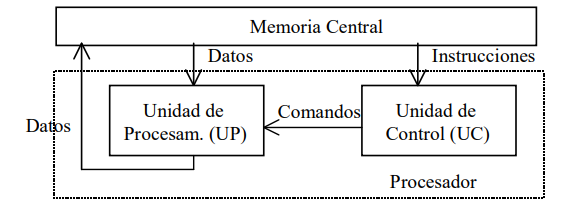
\includegraphics[width=3.18229in,height=1.17579in]{media/image38.png}

\emph{Imagen 3 - SISD}

\textbf{SIMD (Single Instruction Stream, Multiple Data Stream)}

Arreglo de elementos de procesamiento, todos los cuales ejecutan la misma instrucción al mismo tiempo.

El enfoque de paralelismo usado aquí se denomina paralelismo de datos. Los arreglos de procesadores son típicos ejemplos de esta clase de arquitectura. En estas arquitecturas, un controlador recibe y decodifica secuencias de instrucciones a ejecutar, para después enviarlas a múltiples procesadores esclavos.

Su funcionamiento es el siguiente: un simple controlador envía las instrucciones, una a una, a un arreglo de procesadores que operan en el esquema maestro-esclavo. Es decir, las instrucciones son difundidas desde la memoria a un conjunto de procesadores. Así, cada procesador es simplemente una unidad aritmética-lógica y se tiene una sola unidad de control. Todos los procesadores ejecutan cada operación recibida al mismo tiempo, por lo cual, cada uno ejecuta la misma instrucción sobre diferentes datos.

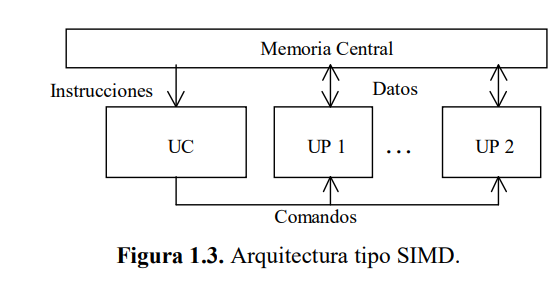
\includegraphics[width=3.19271in,height=1.43274in]{media/image33.png}

\emph{Imagen 4 - SIMD}

\section{Resolución de la ecuación \(f(x)  = x^4 - {5x}^{2} - 2x + 1\) por medio de la Serie de Fourier.}

\subsection{Braulio Gael Porras Zuñiga}

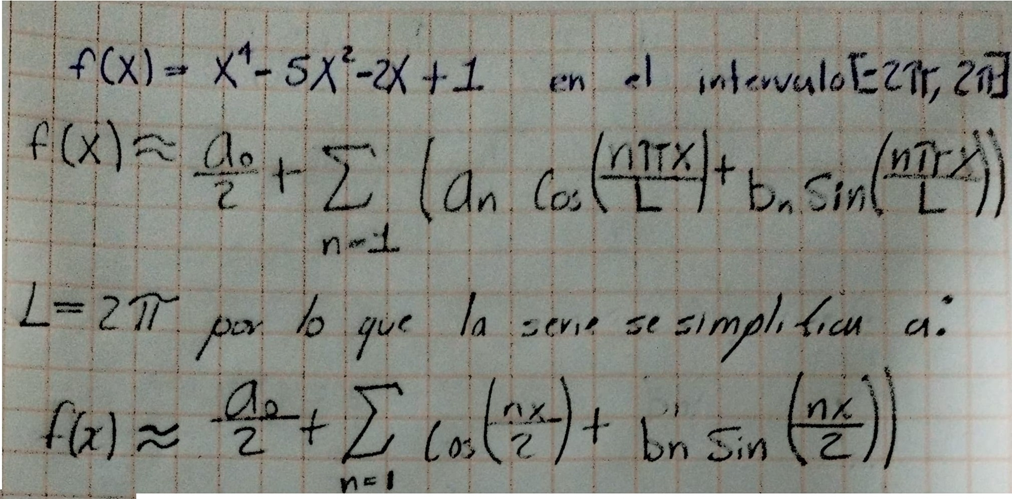
\includegraphics[width=5.15104in,height=2.54129in]{media/image52.png}

Imagen 1A. Procedimiento de Fourier

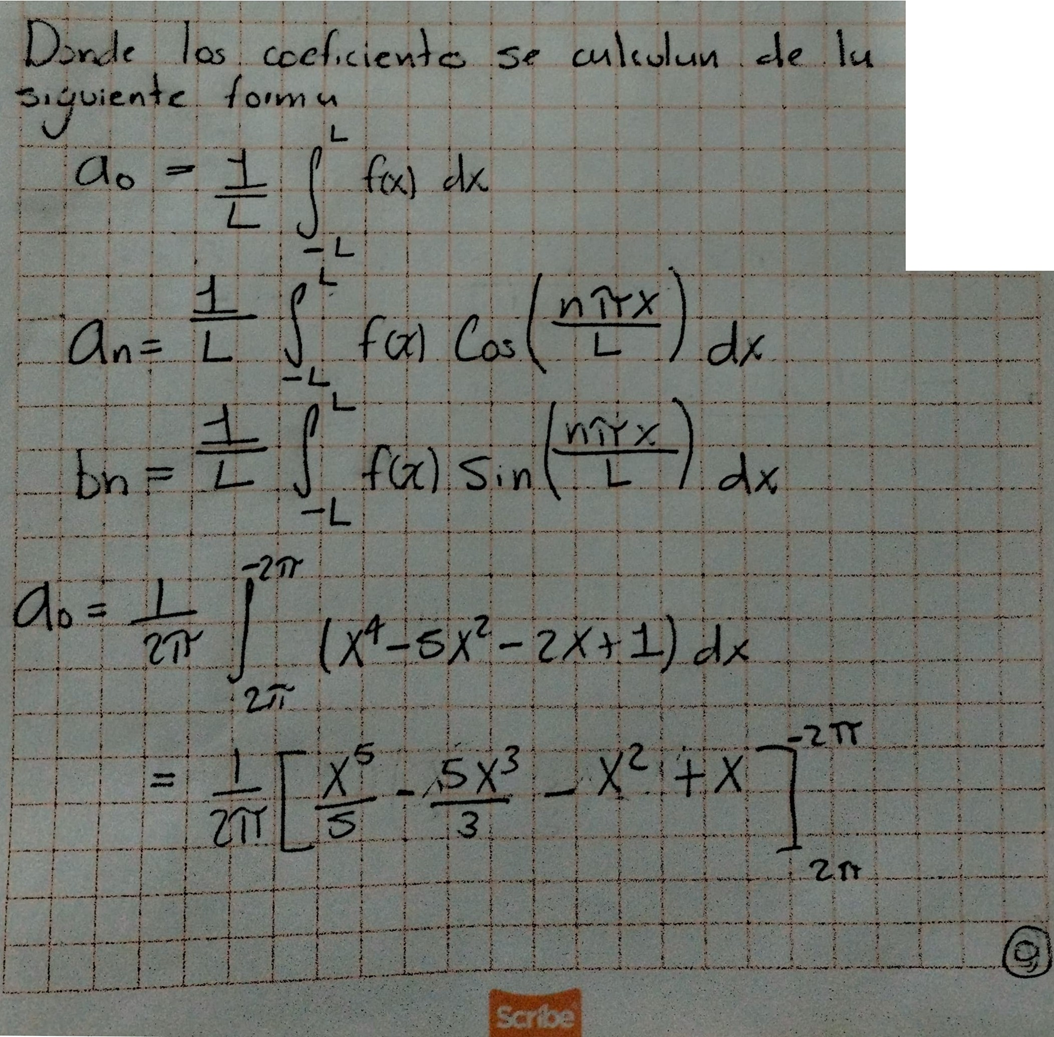
\includegraphics[width=3.66667in,height=3.60643in]{media/image49.png}

Imagen 2A. Procedimiento de Fourier

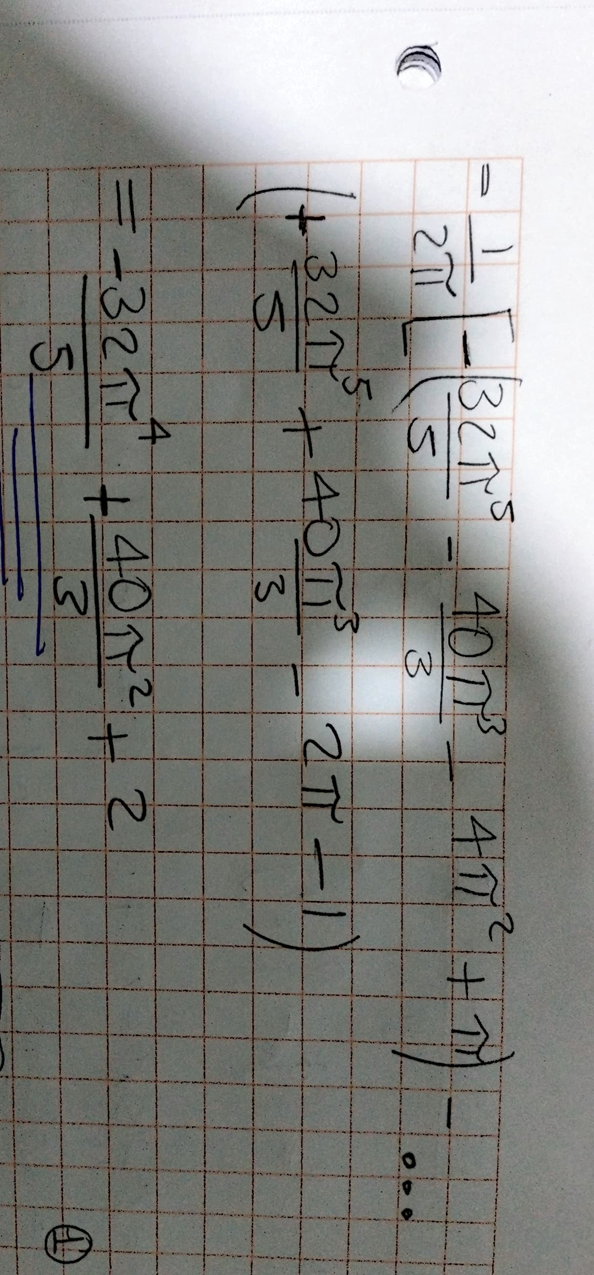
\includegraphics[width=2.34606in,height=5.02604in]{media/image54.png}

Imagen 3A. Procedimiento de Fourier

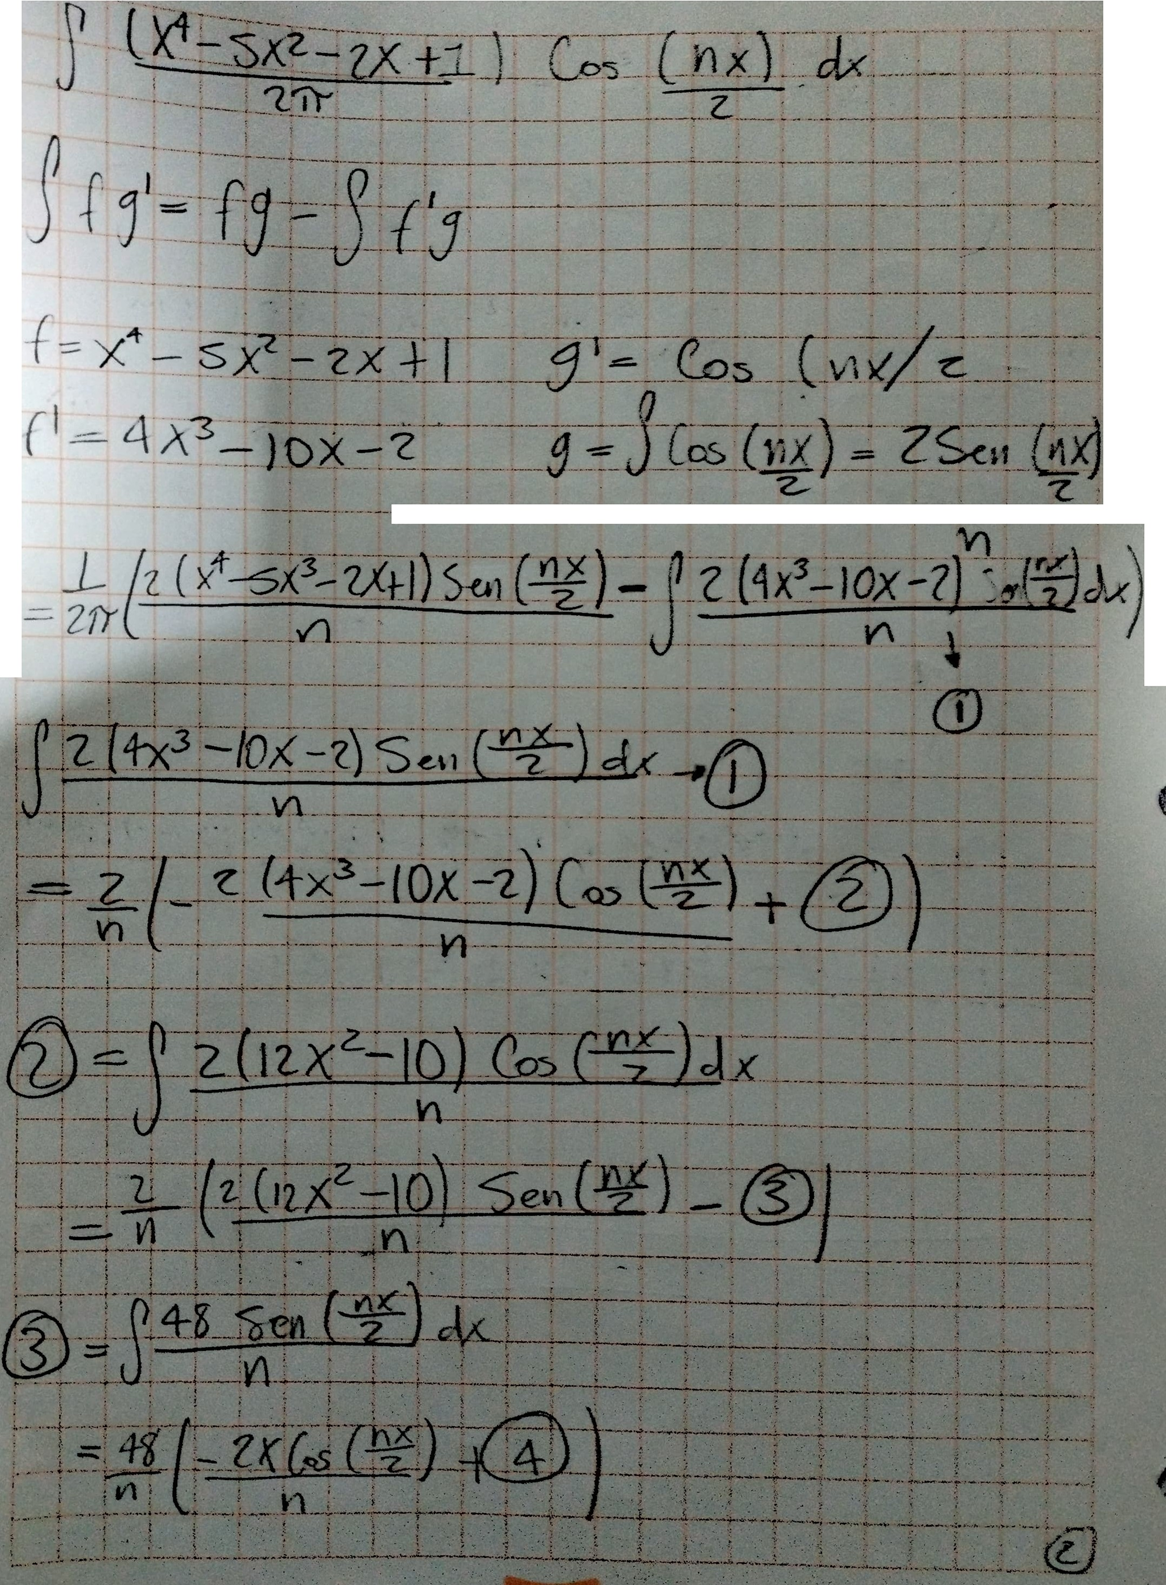
\includegraphics[width=4.84817in,height=6.58854in]{media/image48.png}

Imagen 4A. Procedimiento de Fourier

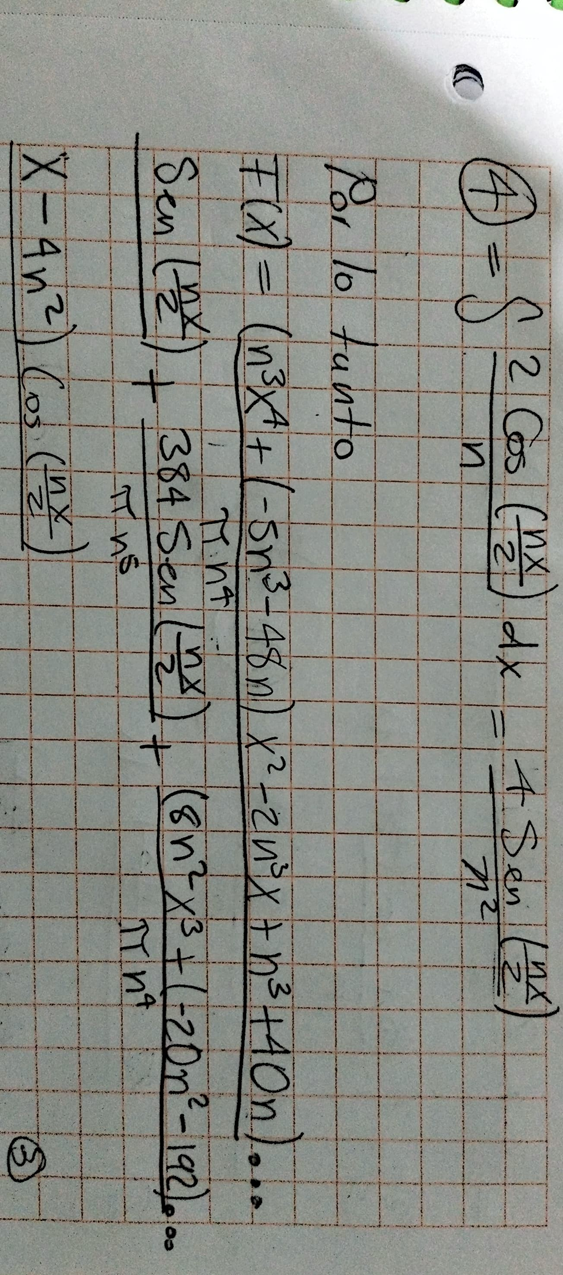
\includegraphics[width=2.15104in,height=4.88023in]{media/image22.png}

Imagen 5A. Procedimiento de Fourier

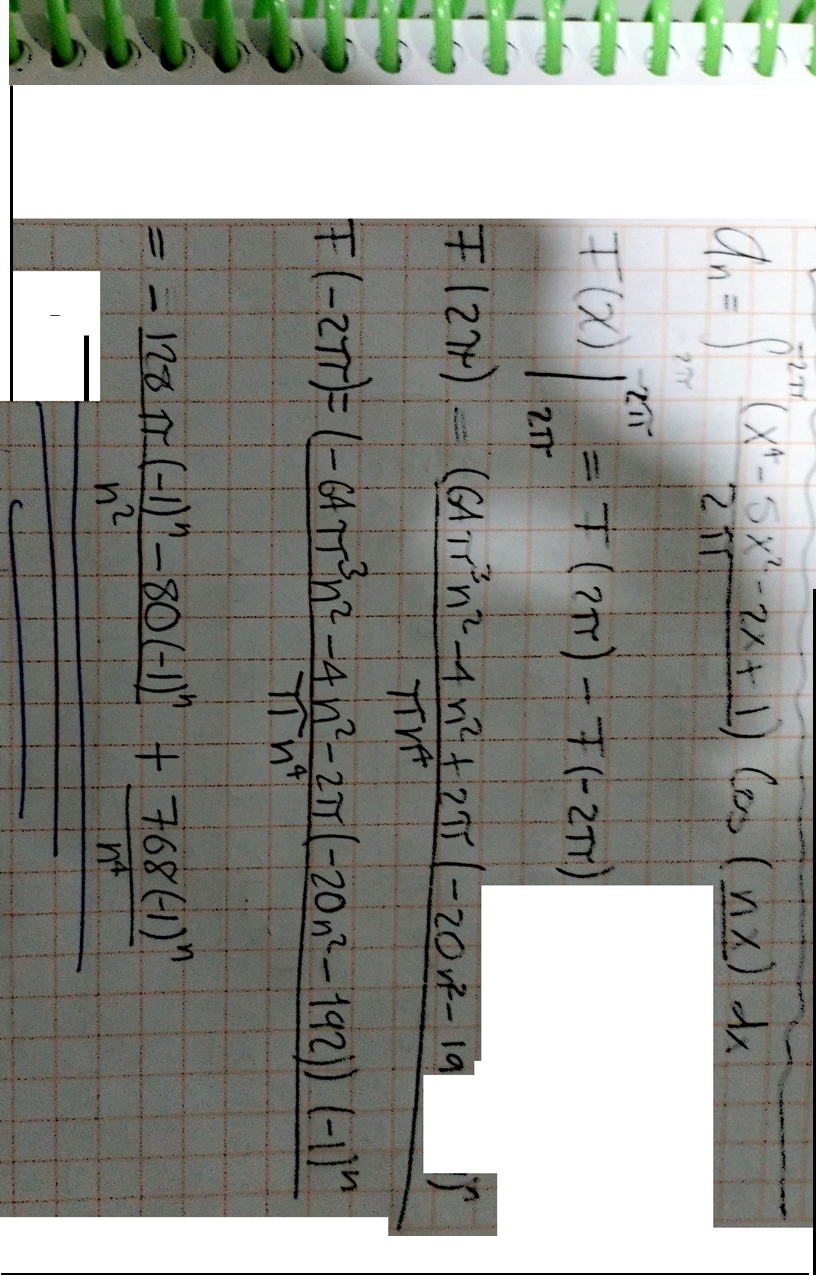
\includegraphics[width=3.07924in,height=4.81771in]{media/image51.png}

Imagen 6A. Procedimiento de Fourier

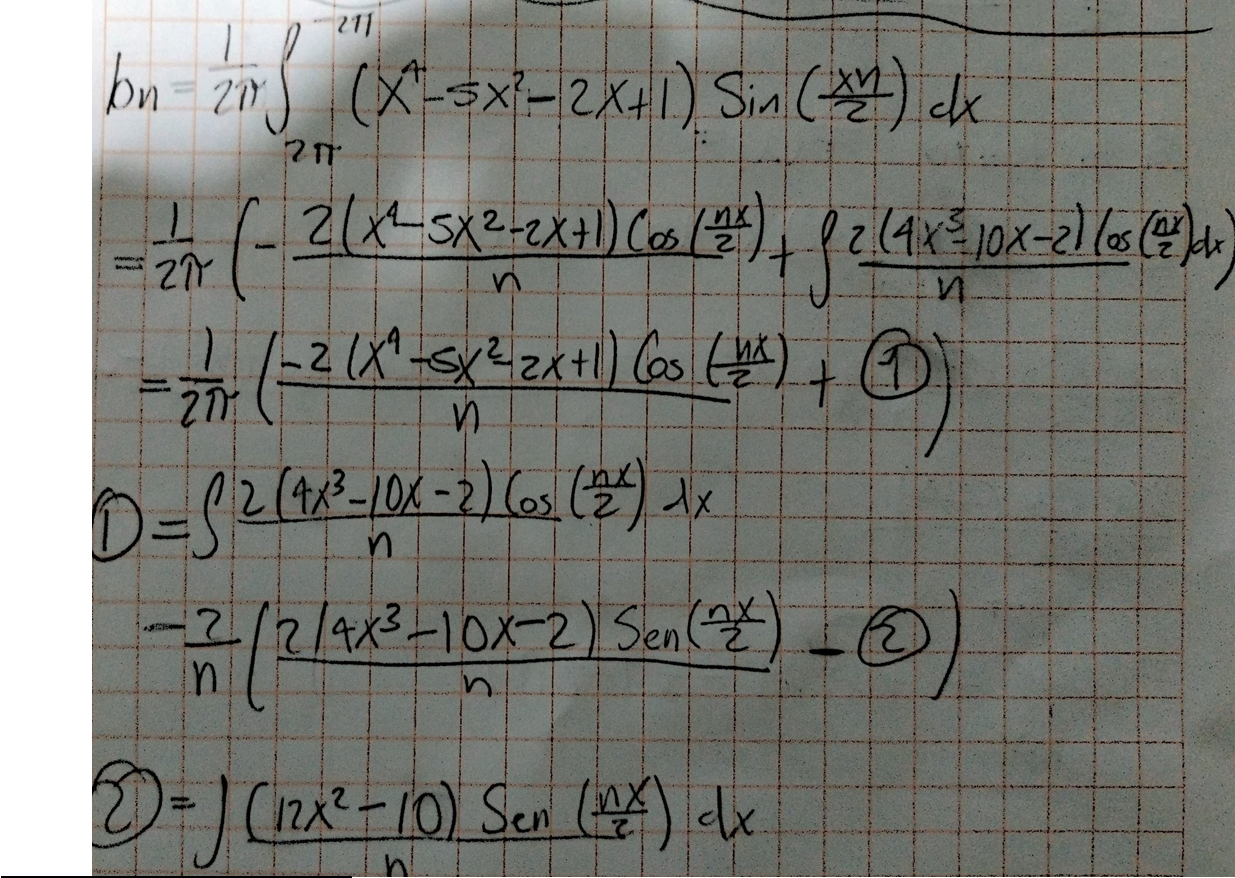
\includegraphics[width=4.74479in,height=3.37337in]{media/image47.png}

Imagen 7A. Procedimiento de Fourier

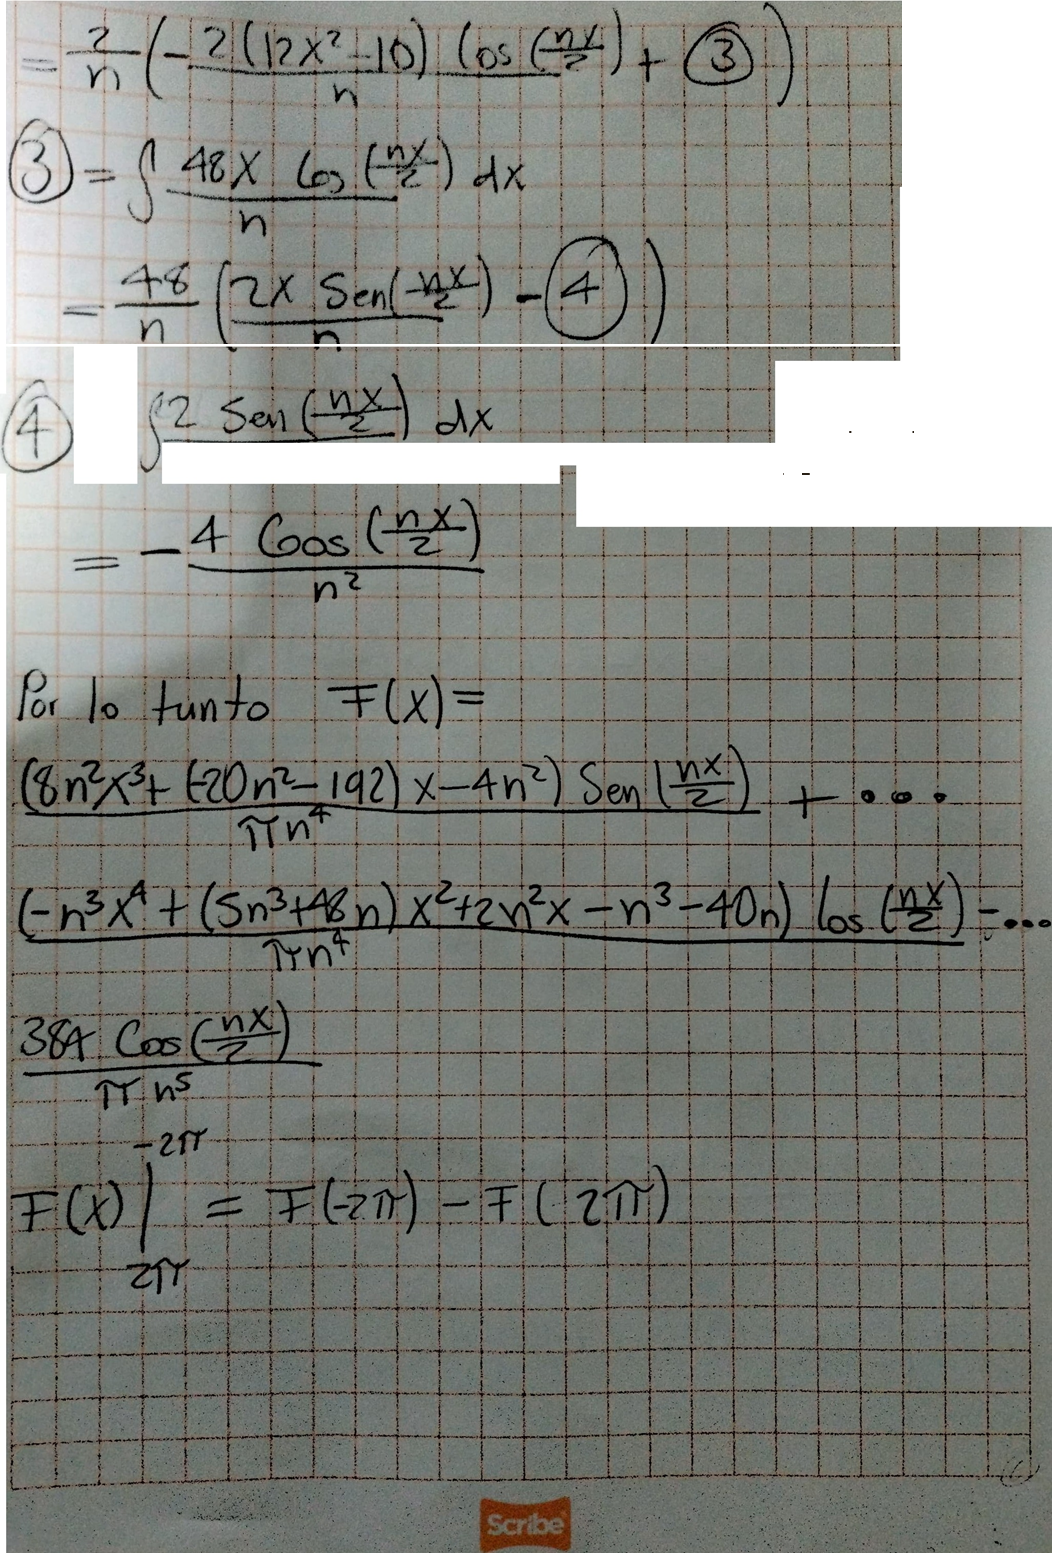
\includegraphics[width=4.94271in,height=7.29091in]{media/image53.png}

Imagen 8A. Procedimiento de Fourier

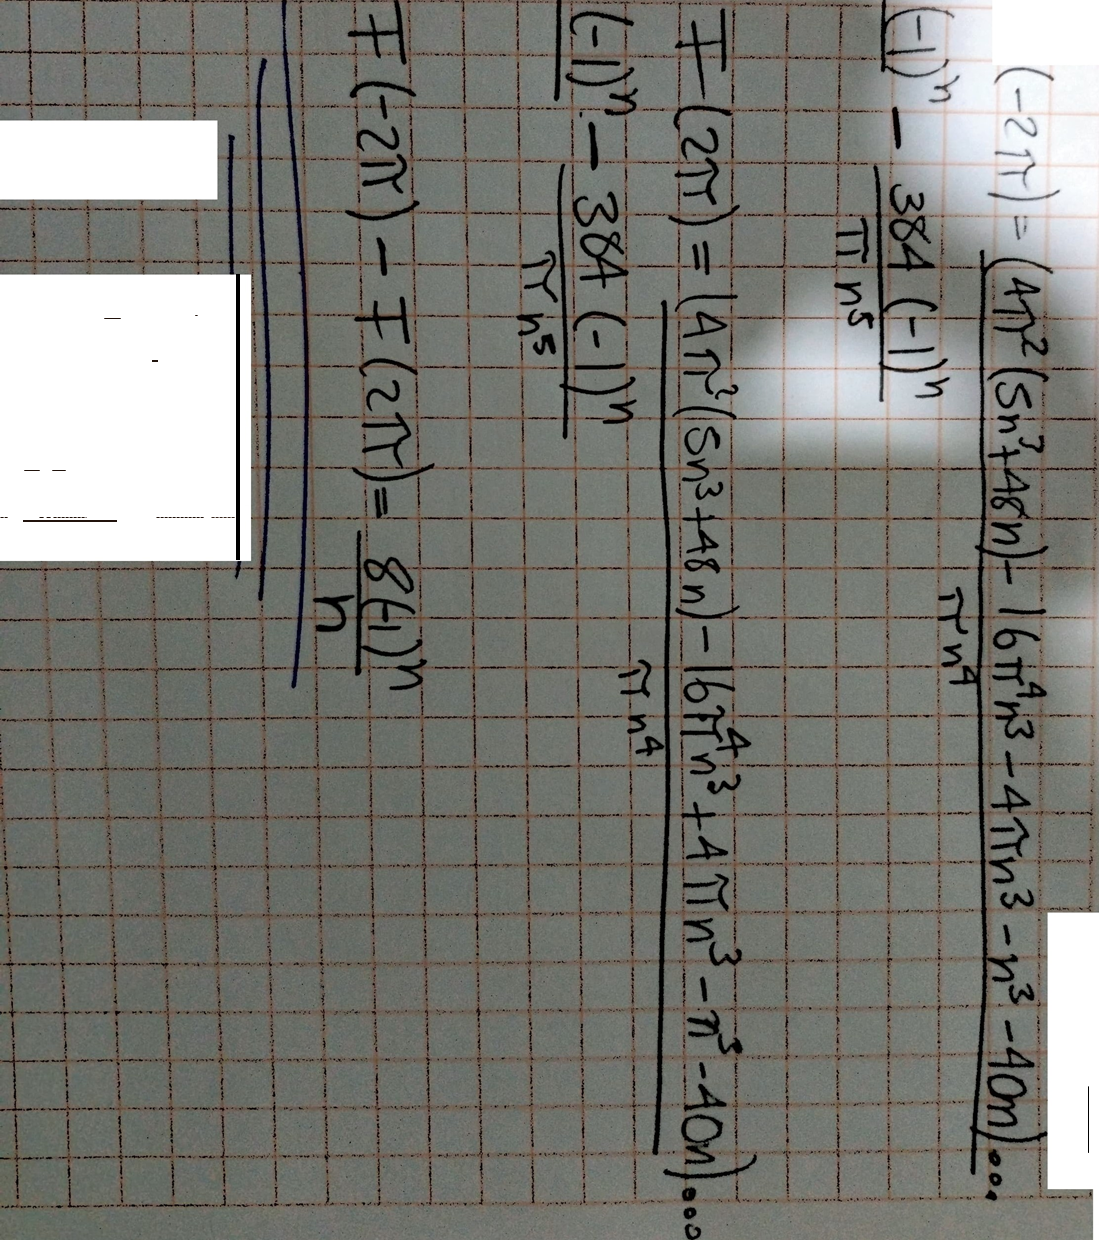
\includegraphics[width=3.88021in,height=4.37099in]{media/image43.png}

Imagen 9A. Procedimiento de Fourier

\subsection{Magaly Citlali Jimeno Reyes}

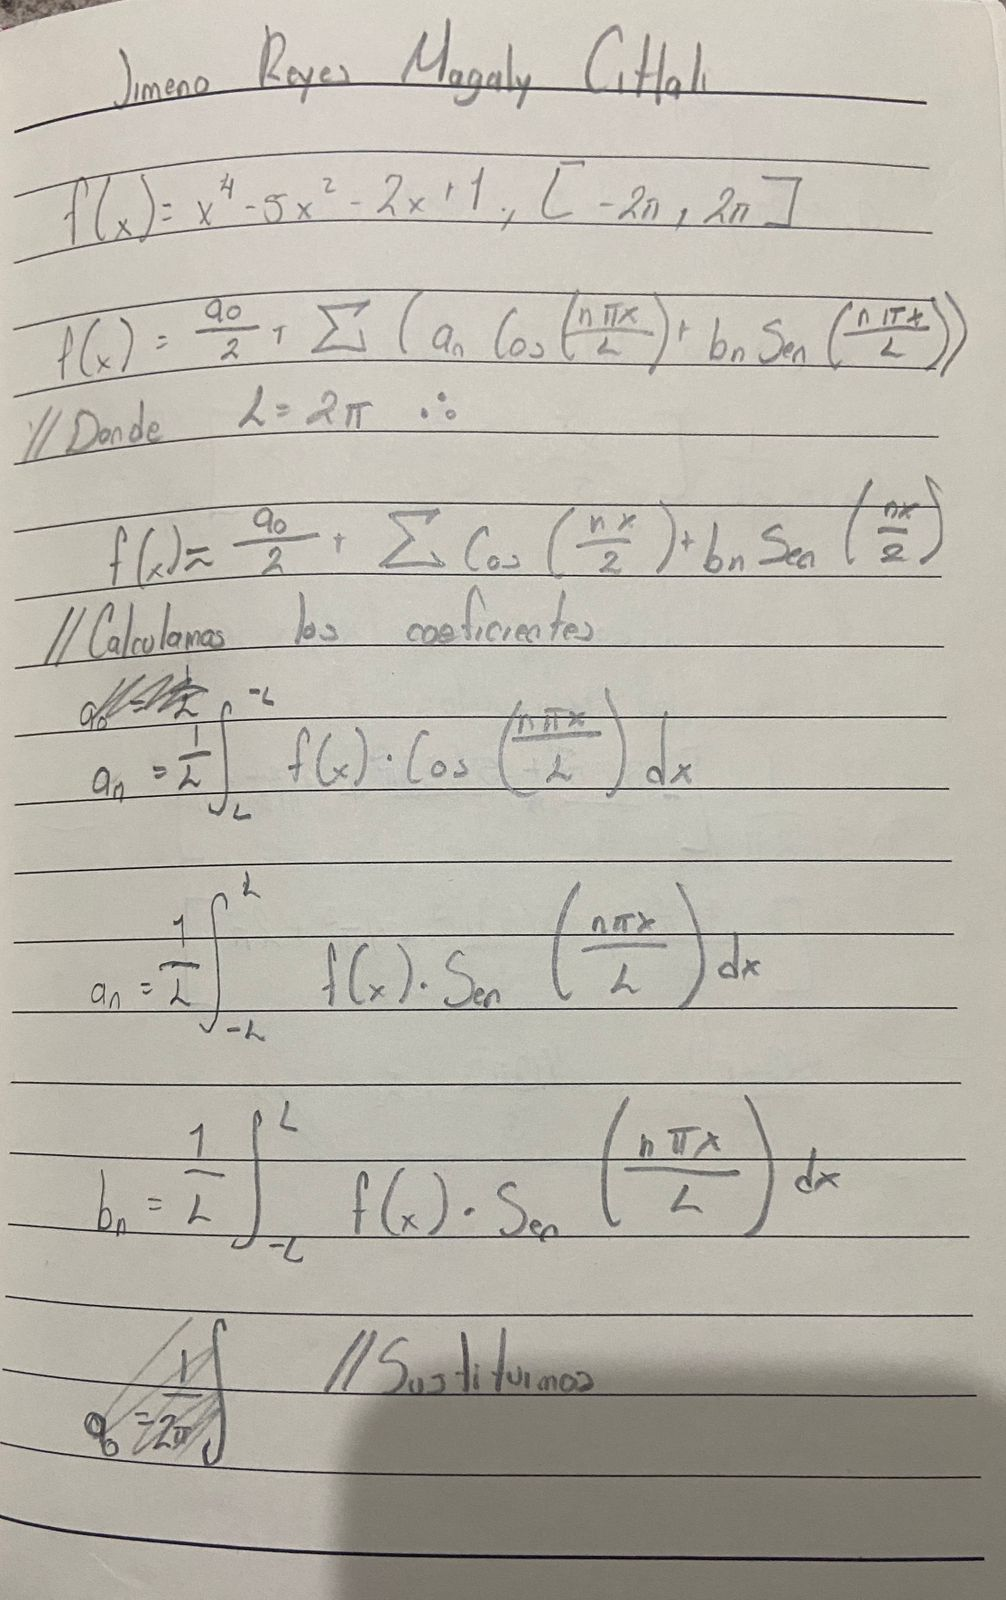
\includegraphics[width=2.98958in,height=4.74434in]{media/image13.jpg}

Imagen 1B. Procedimiento de Fourier

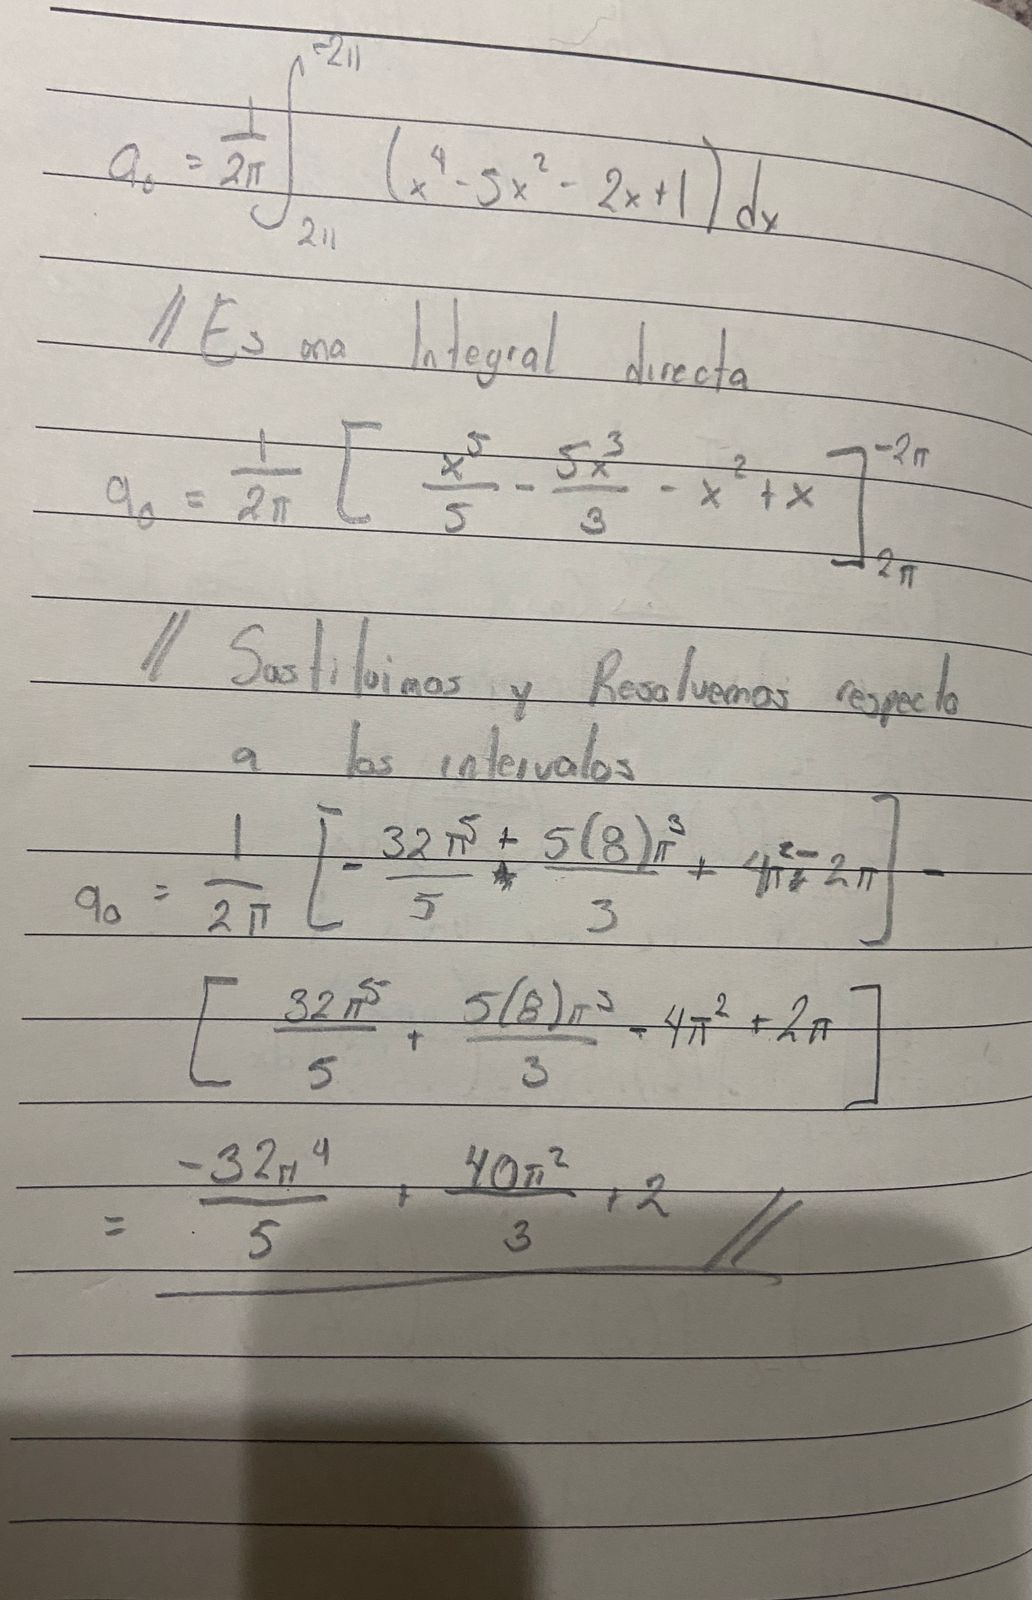
\includegraphics[width=3.03622in,height=4.74409in]{media/image8.jpg}

Imagen 2B. Procedimiento de Fourier

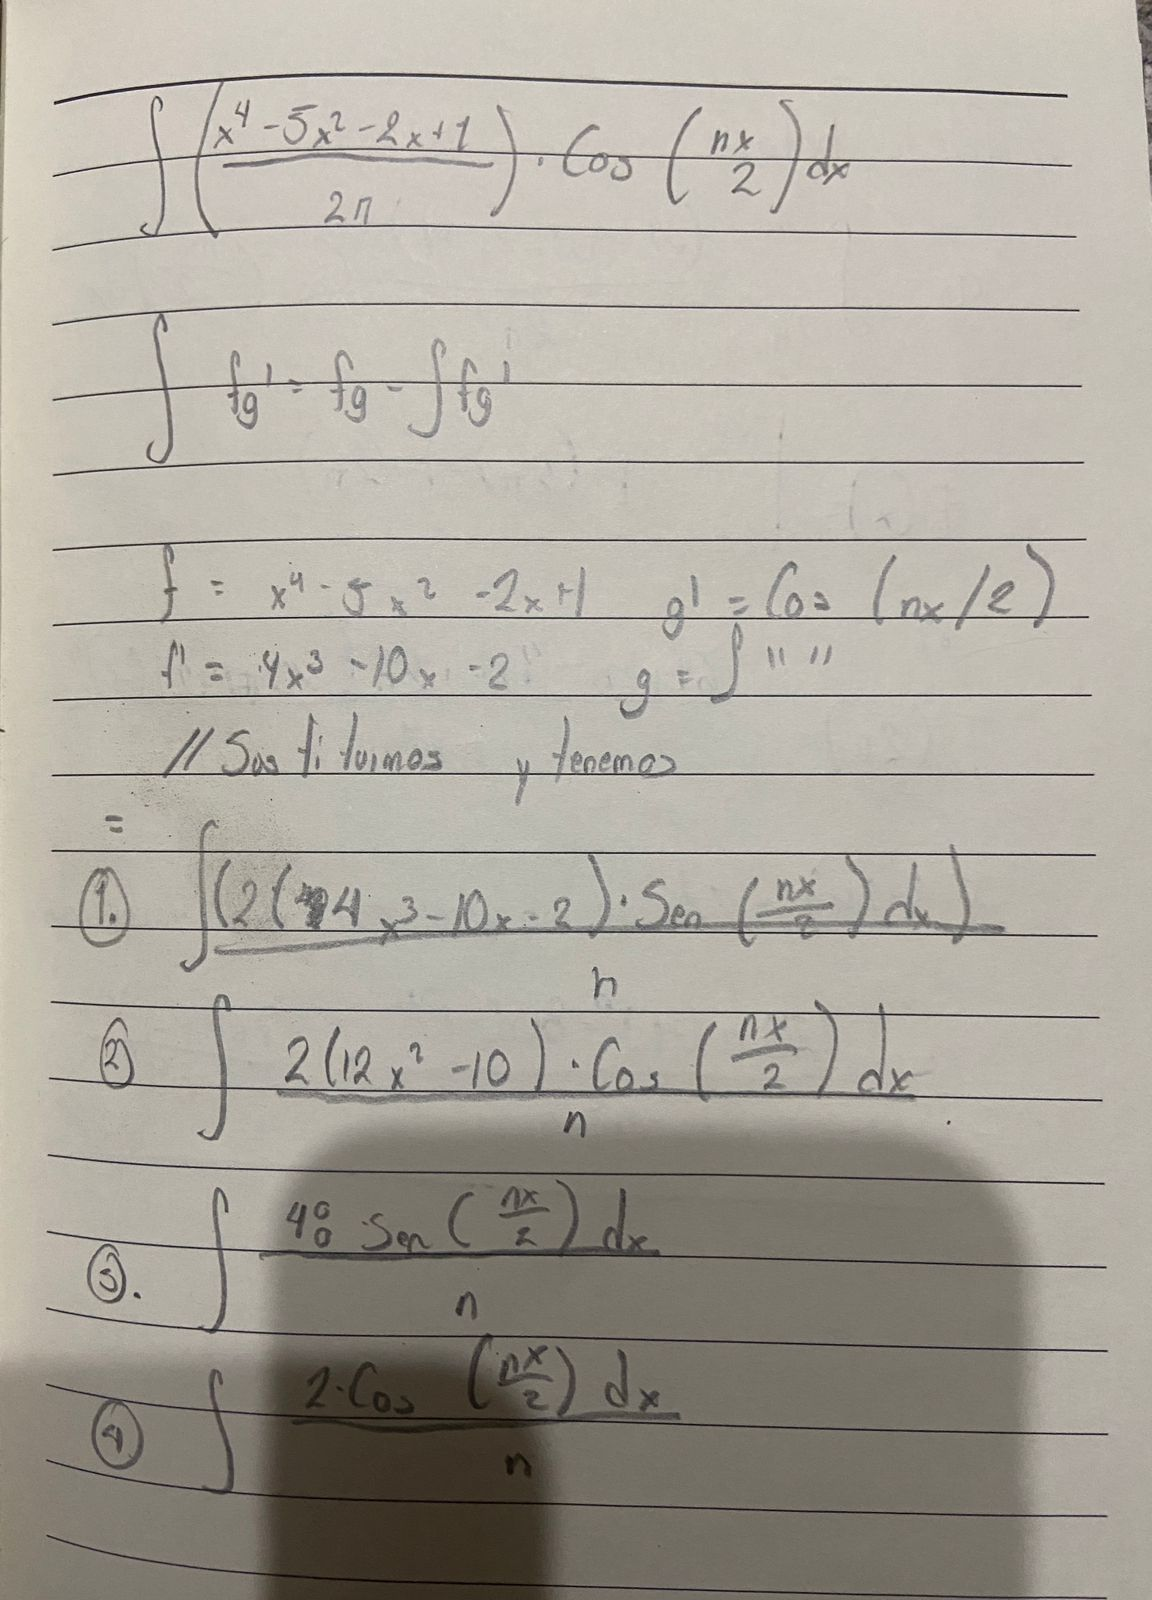
\includegraphics[width=3.0625in,height=5.18146in]{media/image42.jpg}

Imagen 3B. Procedimiento de Fourier

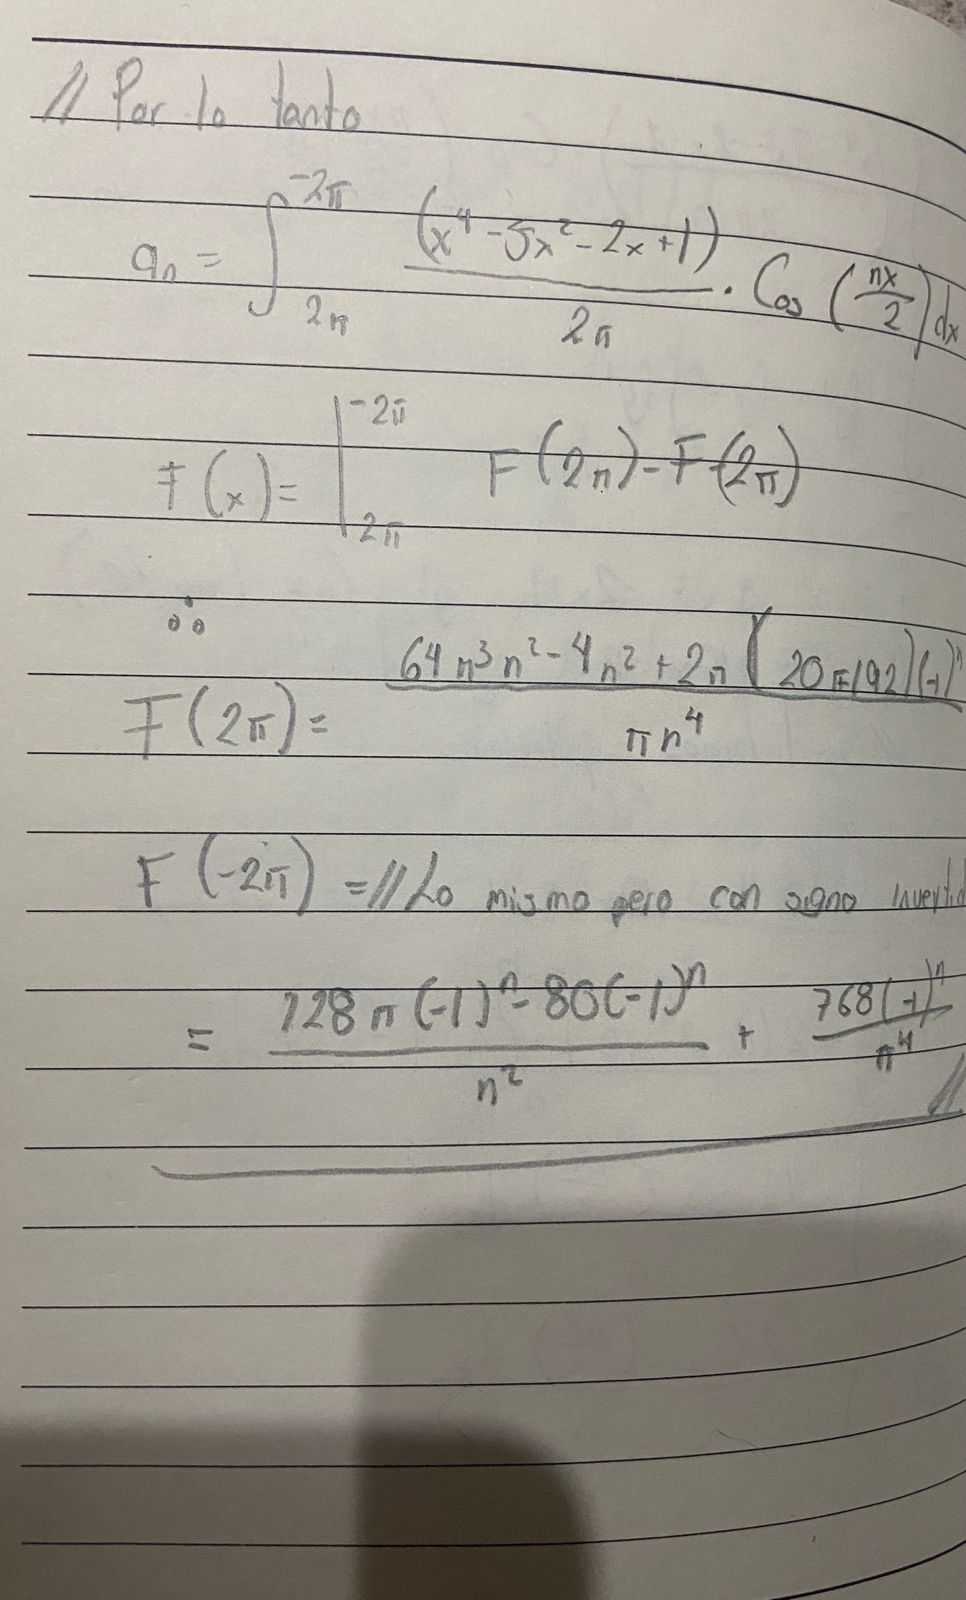
\includegraphics[width=2.97297in,height=4.92052in]{media/image2.jpg}

Imagen 4B. Procedimiento de Fourier

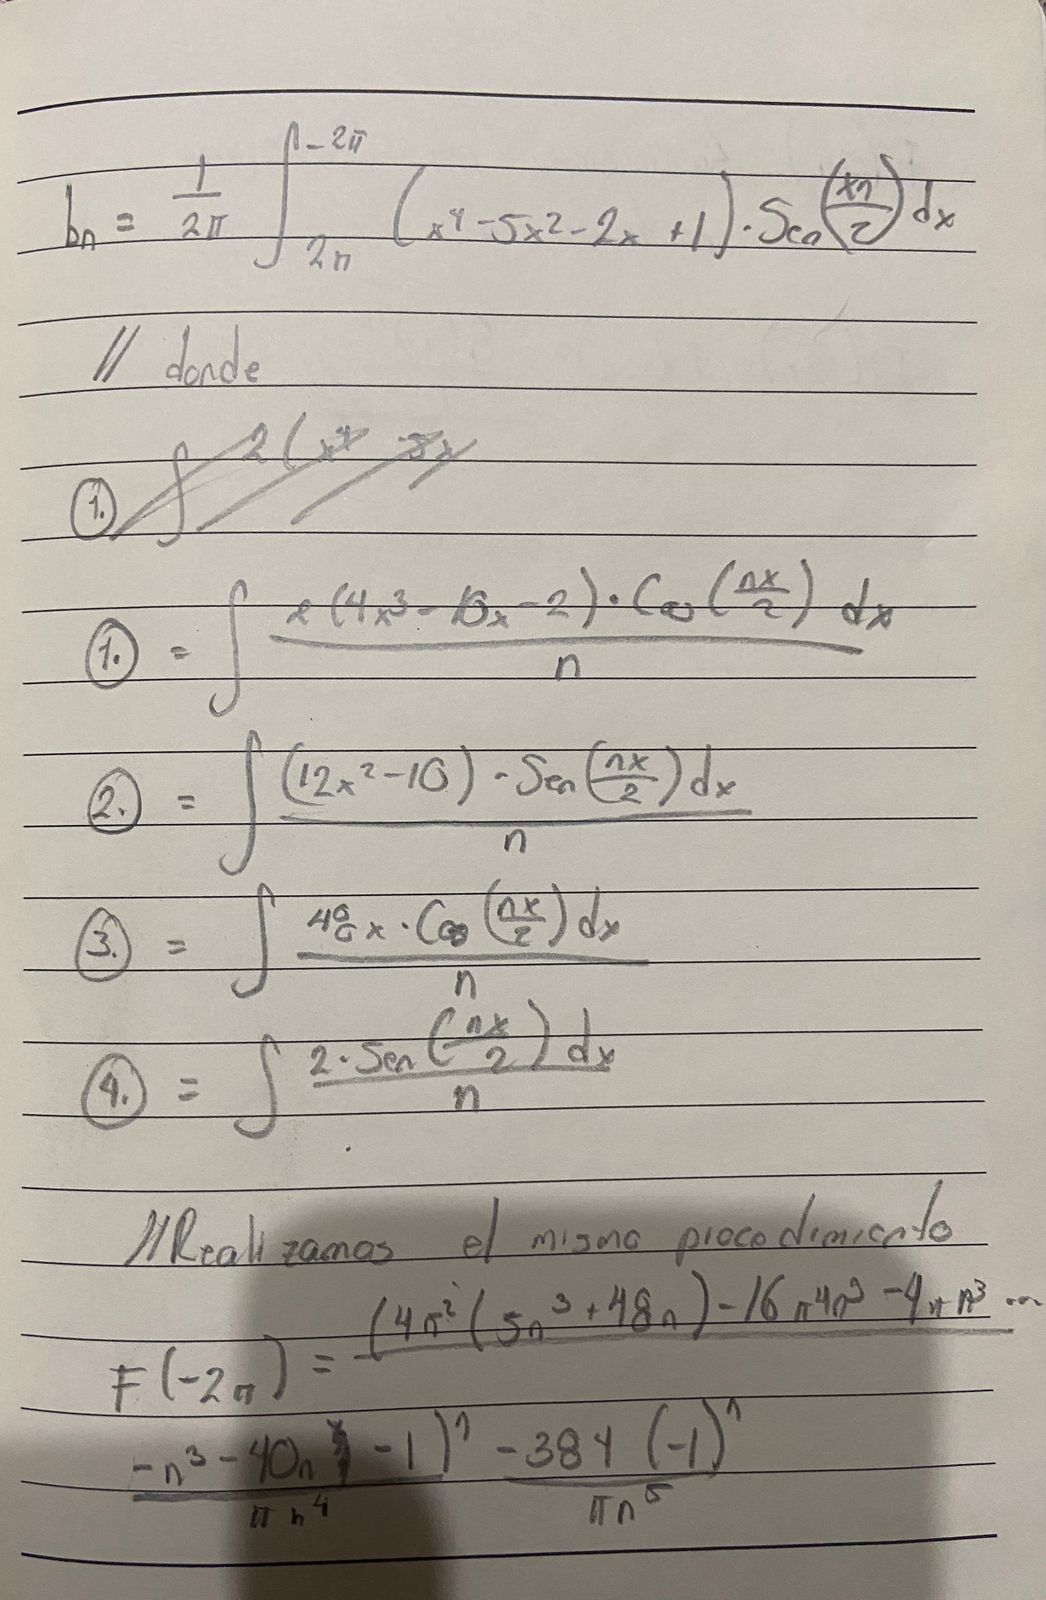
\includegraphics[width=3.1436in,height=4.80787in]{media/image9.jpg}

Imagen 5B. Procedimiento de Fourier

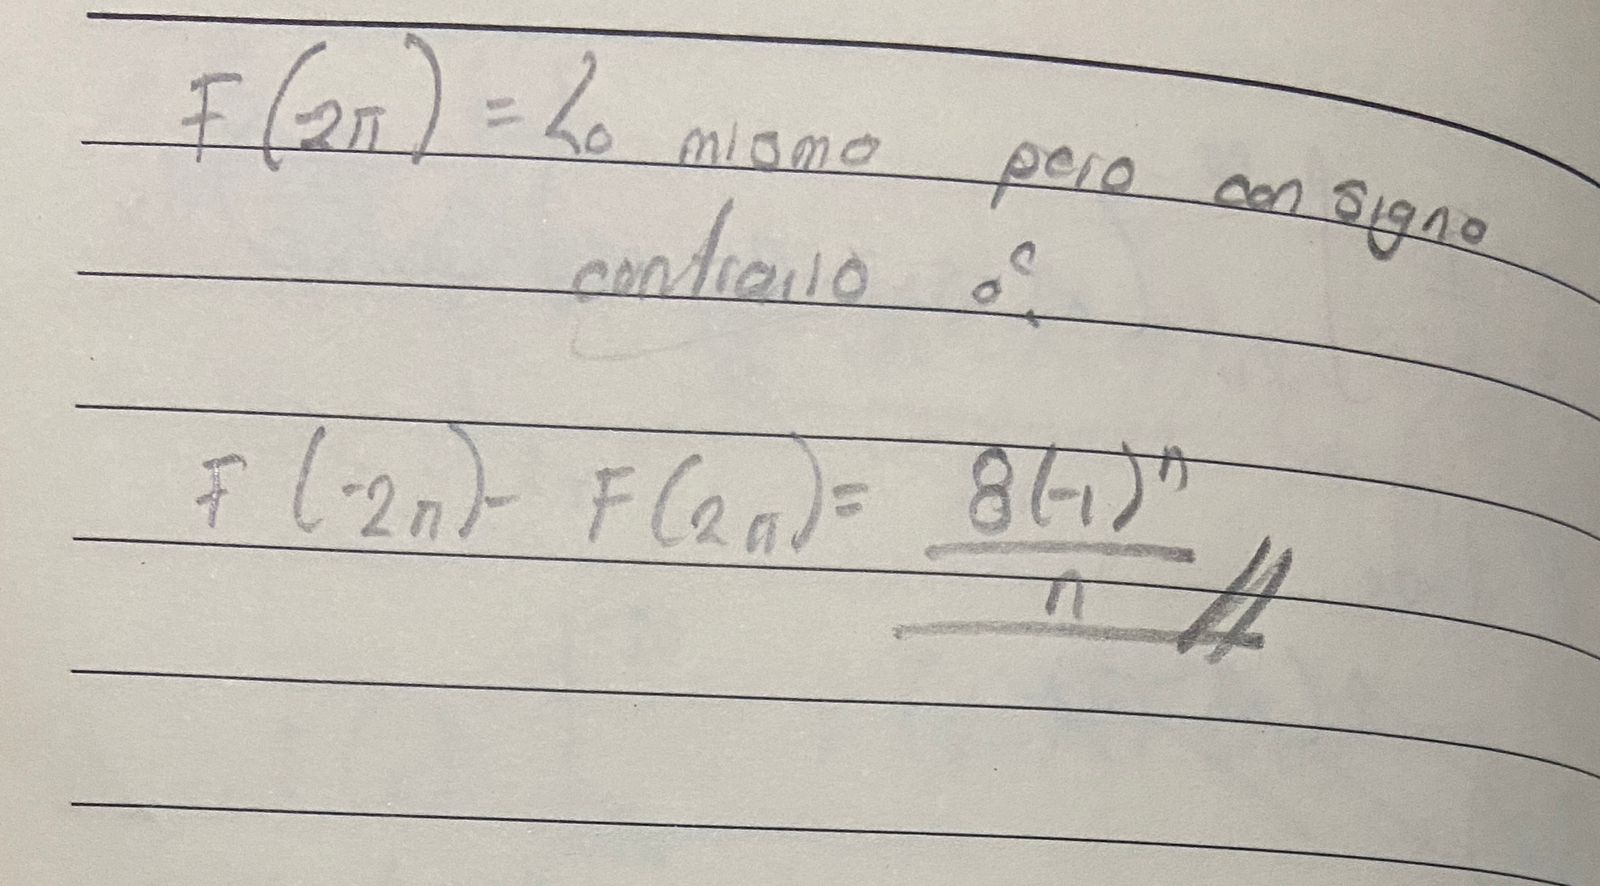
\includegraphics[width=3.00684in,height=3.1593in]{media/image46.jpg}

Imagen 6B. Procedimiento de Fourier

\subsection{Juárez Botello Josué Adalid}

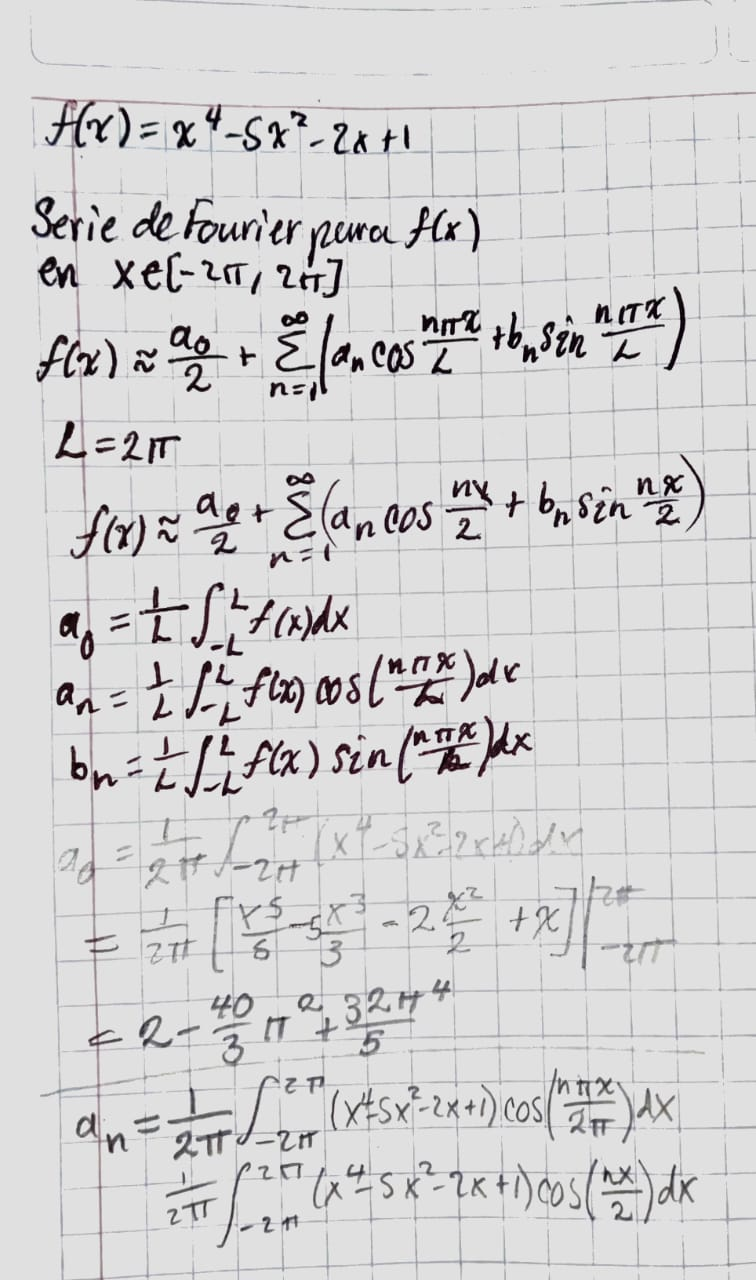
\includegraphics[width=3.19696in,height=5.41146in]{media/image44.jpg}\\ Imagen C1. Primero, establecemos la forma de la serie de la función f(x).

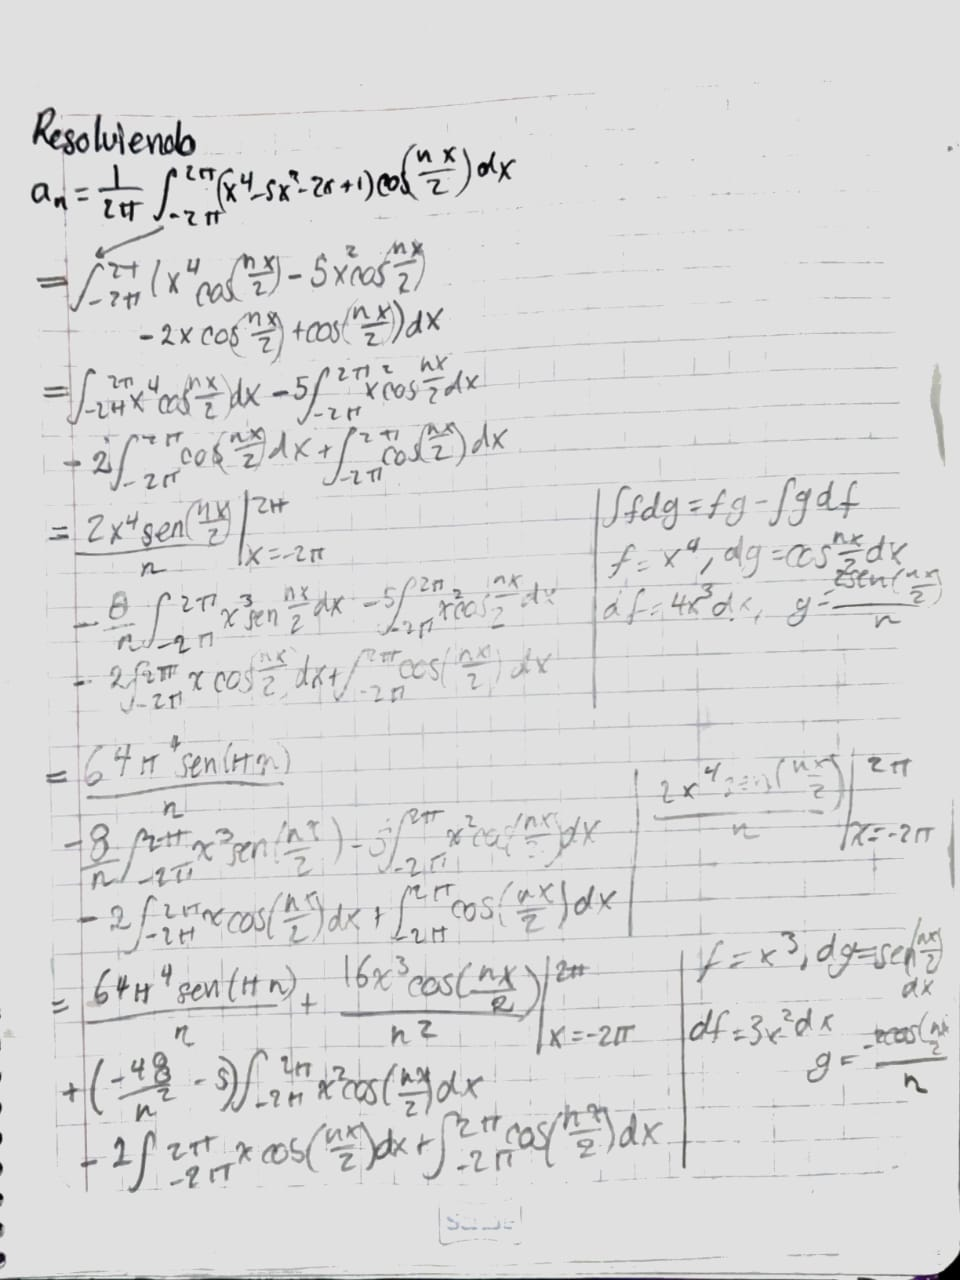
\includegraphics[width=3.12761in,height=4.17188in]{media/image31.jpg}\\ Imagen C2. Primero determinaremos la forma cerrada del término a\_n.

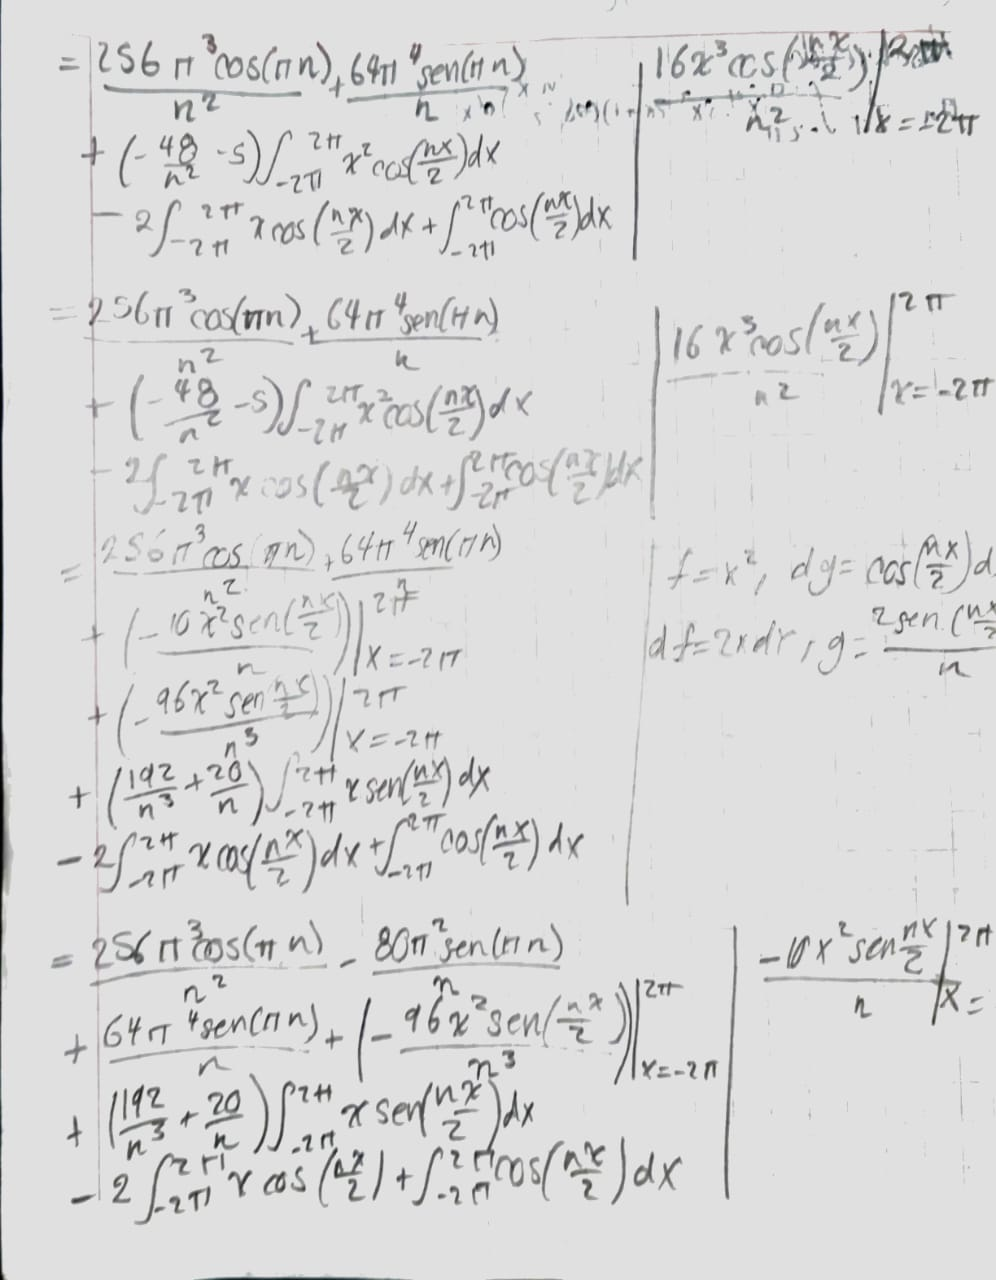
\includegraphics[width=2.78659in,height=3.57813in]{media/image34.jpg}

Imagen C3. continuación del cálculo a\_n.

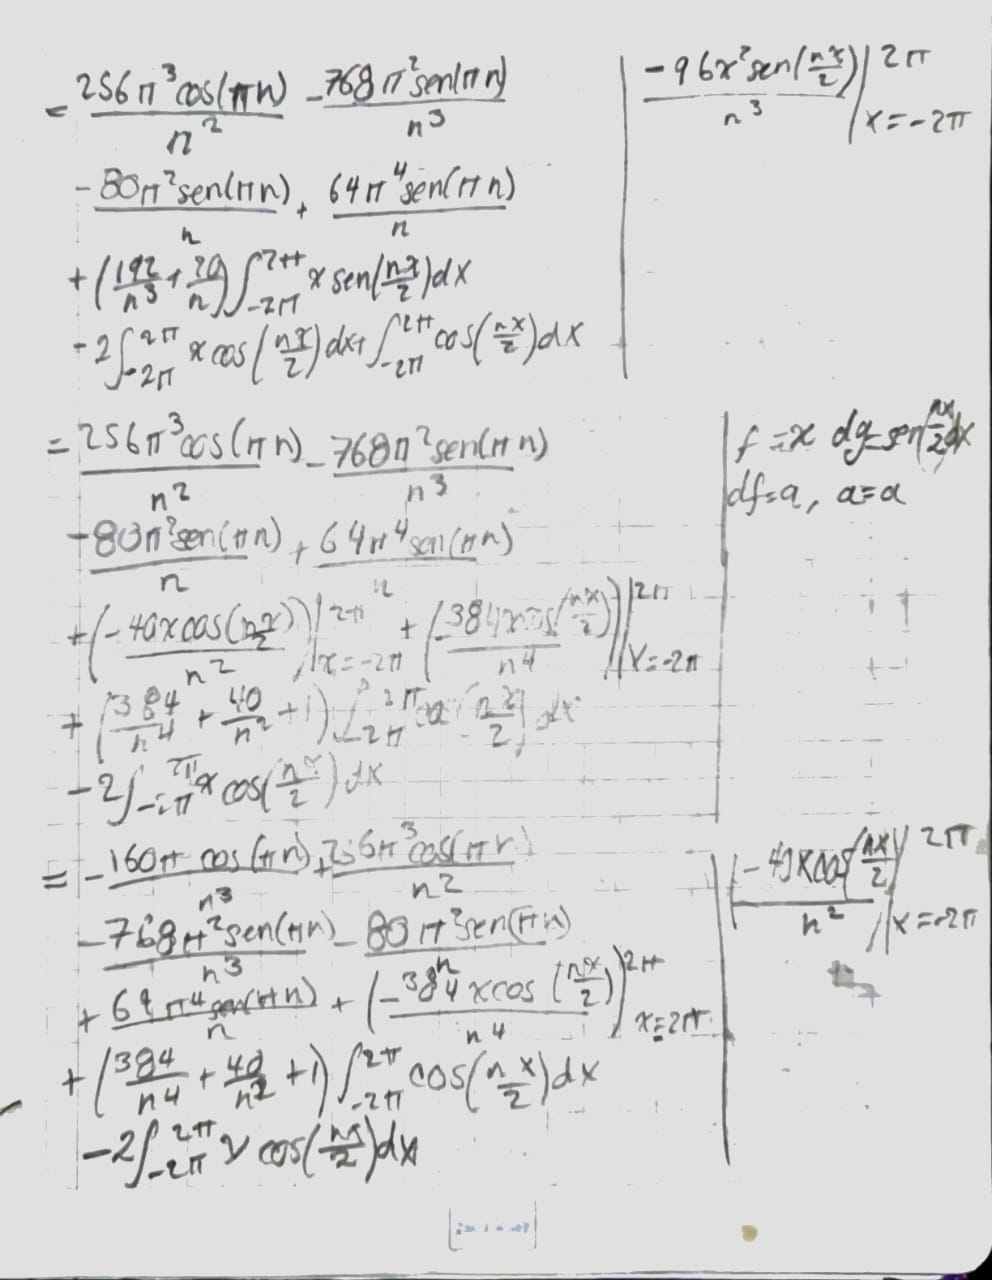
\includegraphics[width=2.84046in,height=3.66146in]{media/image14.jpg}\\ Imagen C4. Continuación cálculo a\_n.

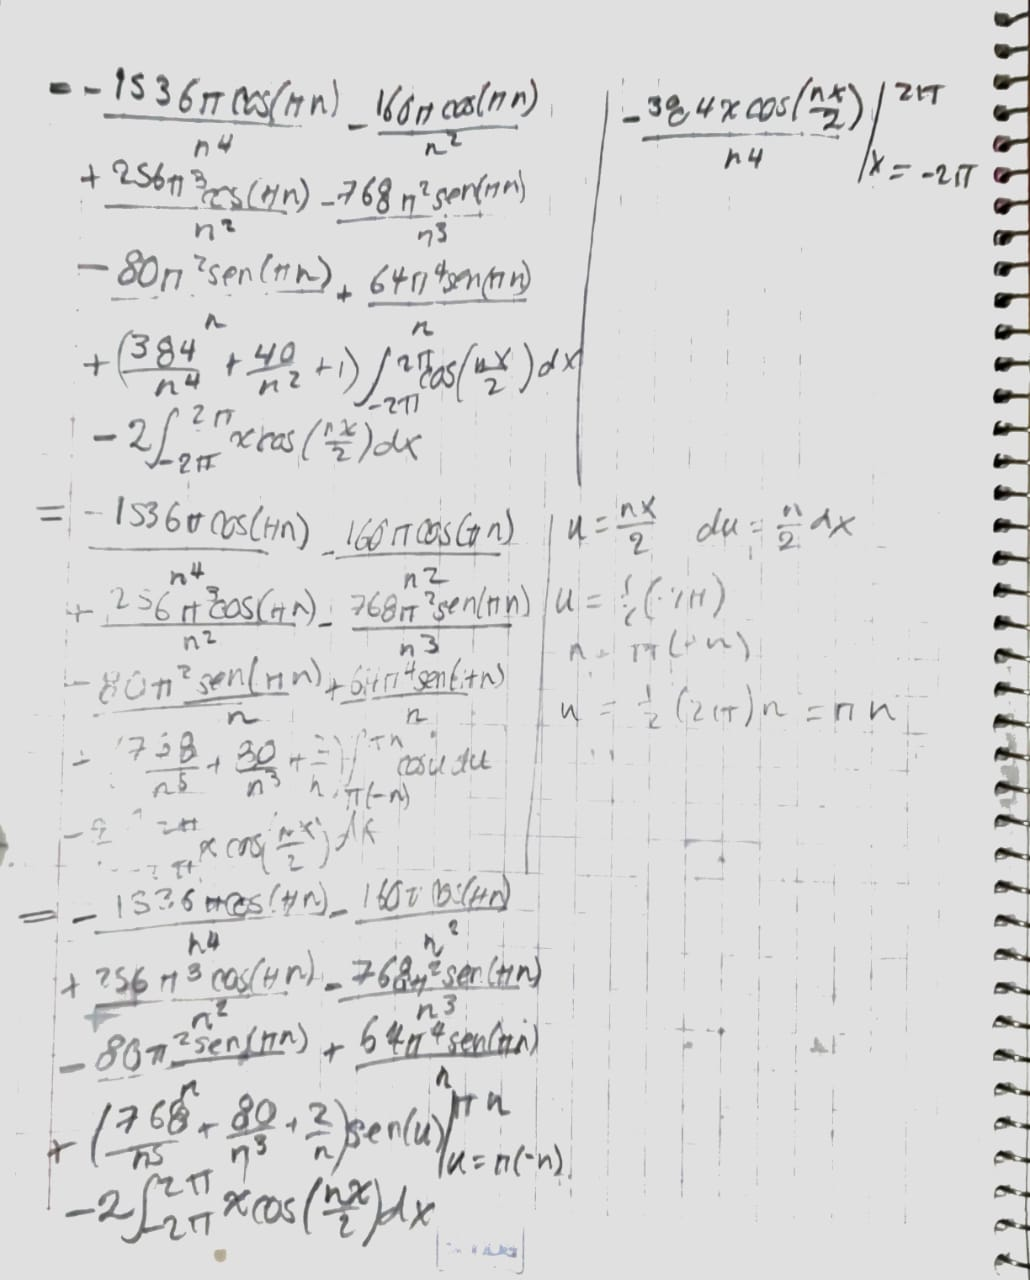
\includegraphics[width=2.66175in,height=3.30729in]{media/image15.jpg}

Imagen C5. Continuación cálculo a\_n.

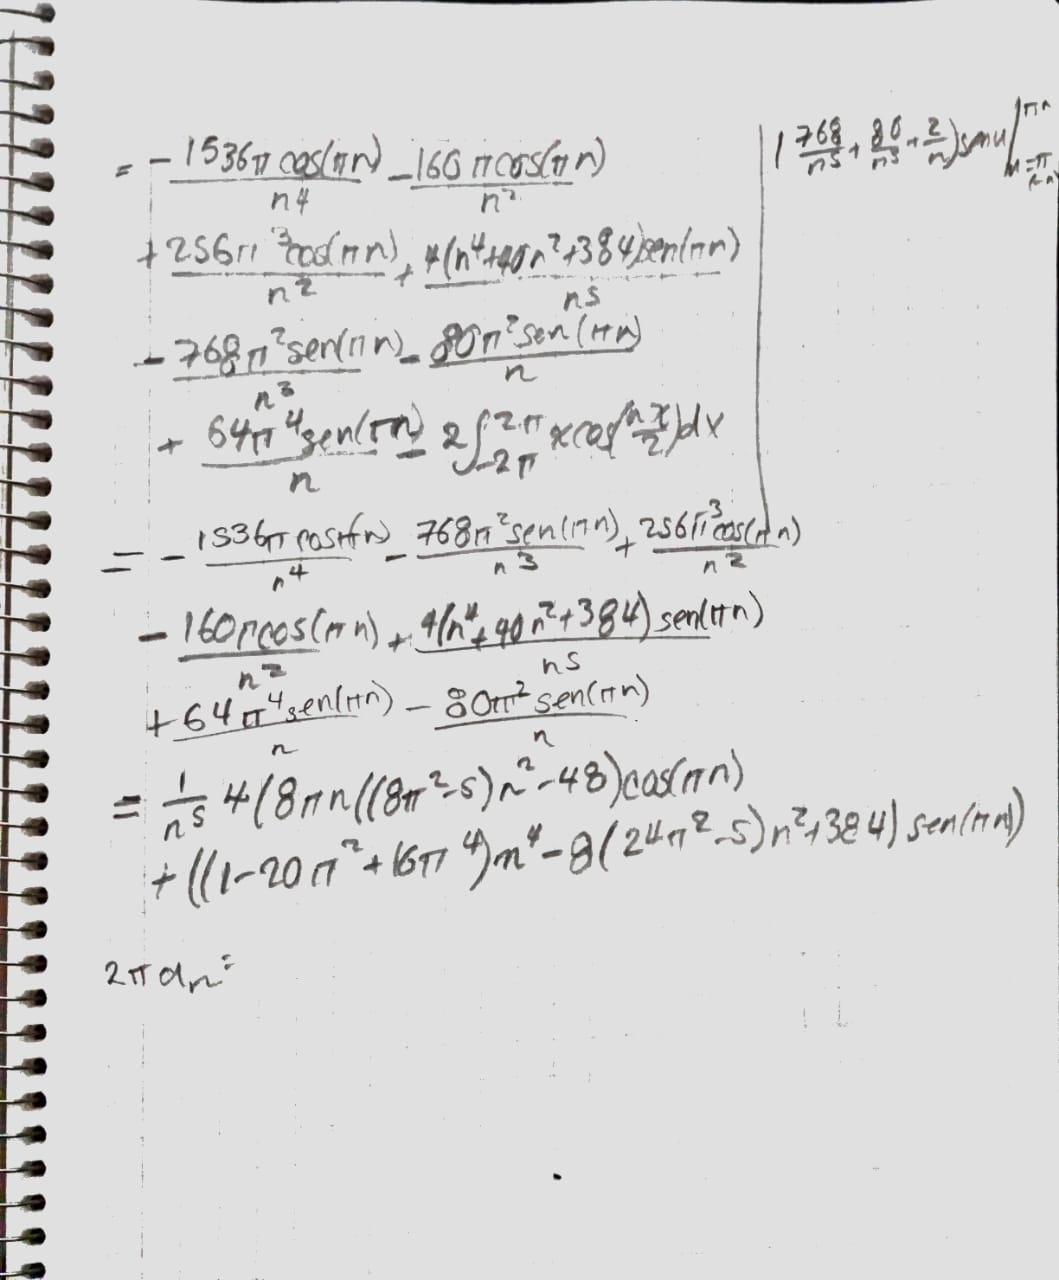
\includegraphics[width=3.09896in,height=3.74243in]{media/image45.jpg}\\ Imagen C6. Finalmente, definimos que el término a\_n es igual a lo que se muestra en la foto.

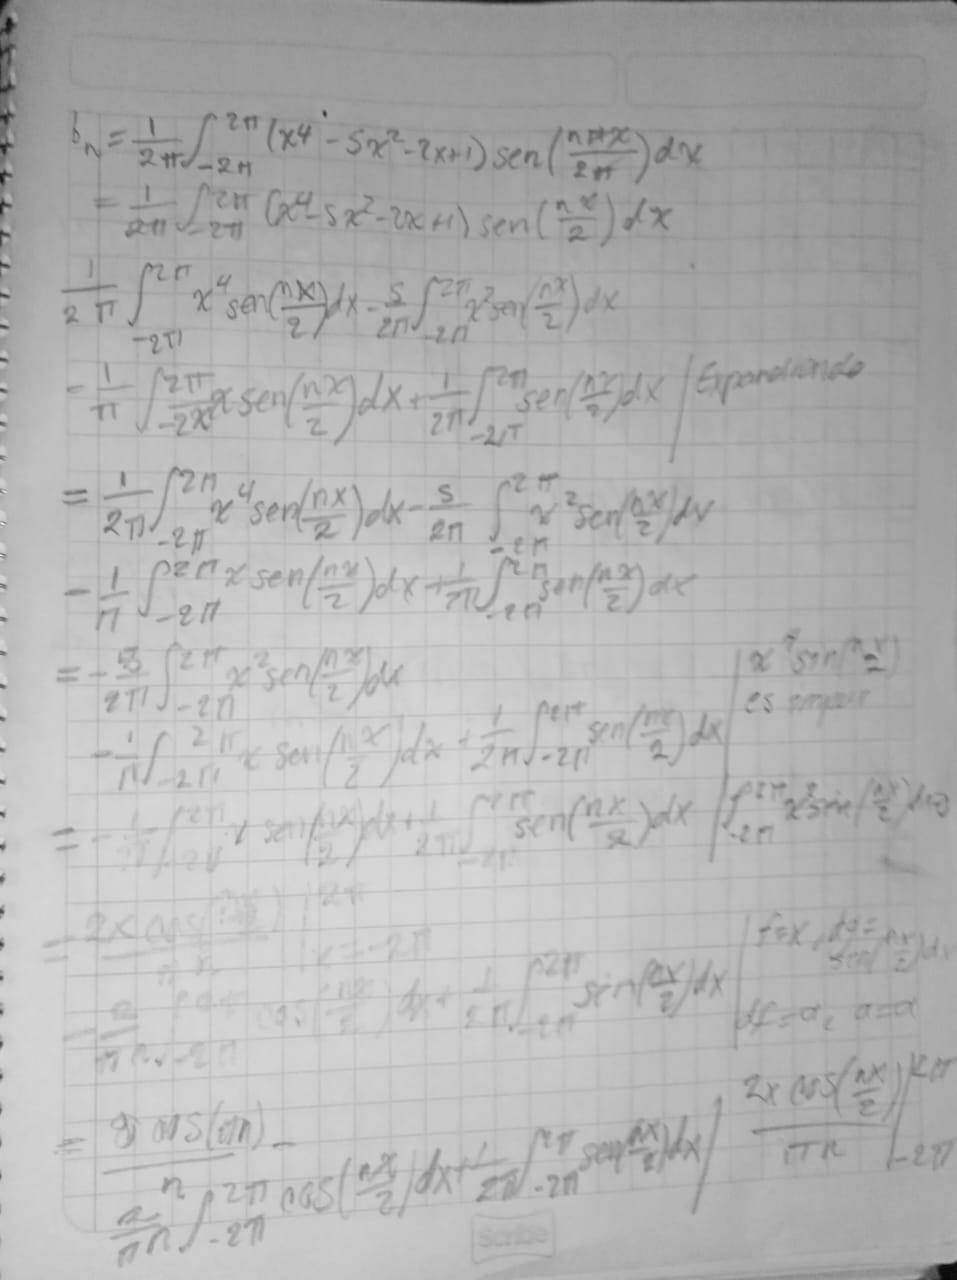
\includegraphics[width=2.6836in,height=3.58854in]{media/image26.jpg}\\ Imagen C7. Continuamos con la determinación del término b\_n

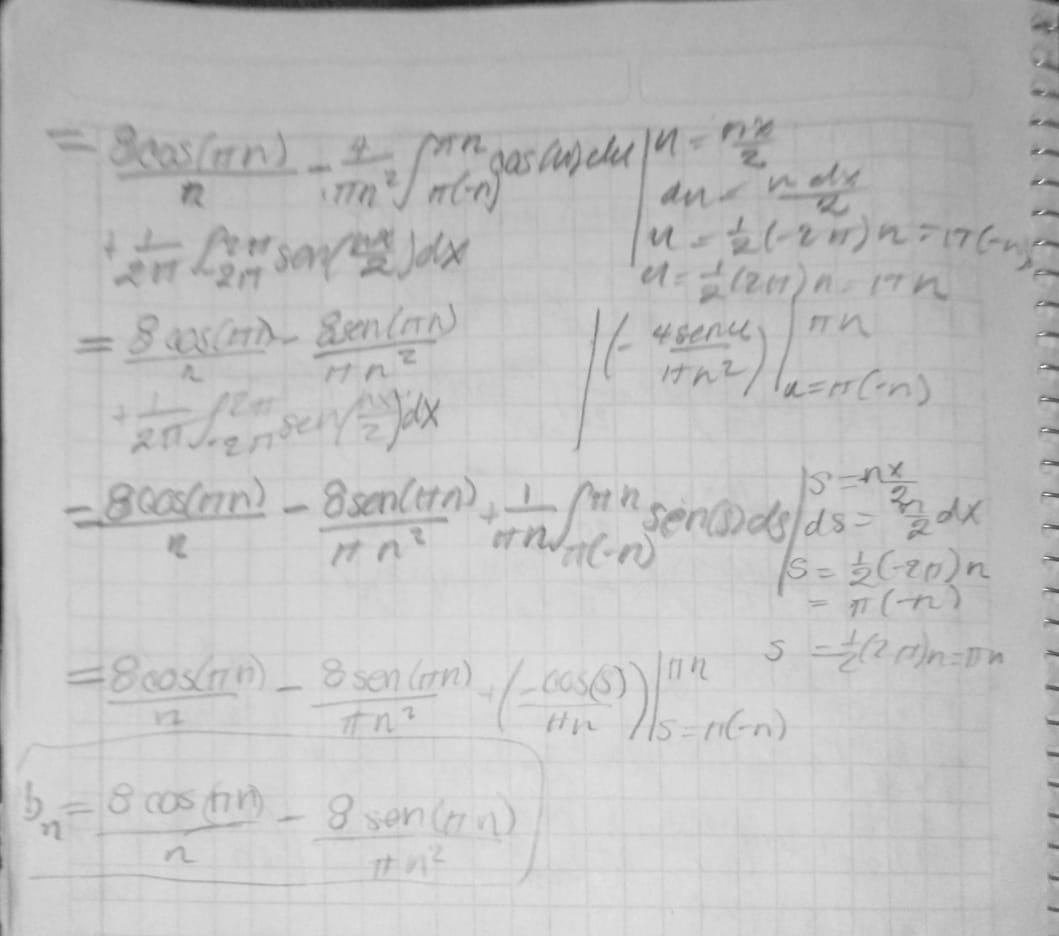
\includegraphics[width=4.00521in,height=3.53949in]{media/image41.jpg}\\ Imagen C8. Y ese es el término b\_n para la serie de Fourier. Sustituímos en la forma de la serie mencionada al principio. Cabe señalar que fue mucho más sencillo calcular b\_n por la propiedad de la función seno de ser impar.

\subsection{Oscar Uriel Juarez Tolamatl}

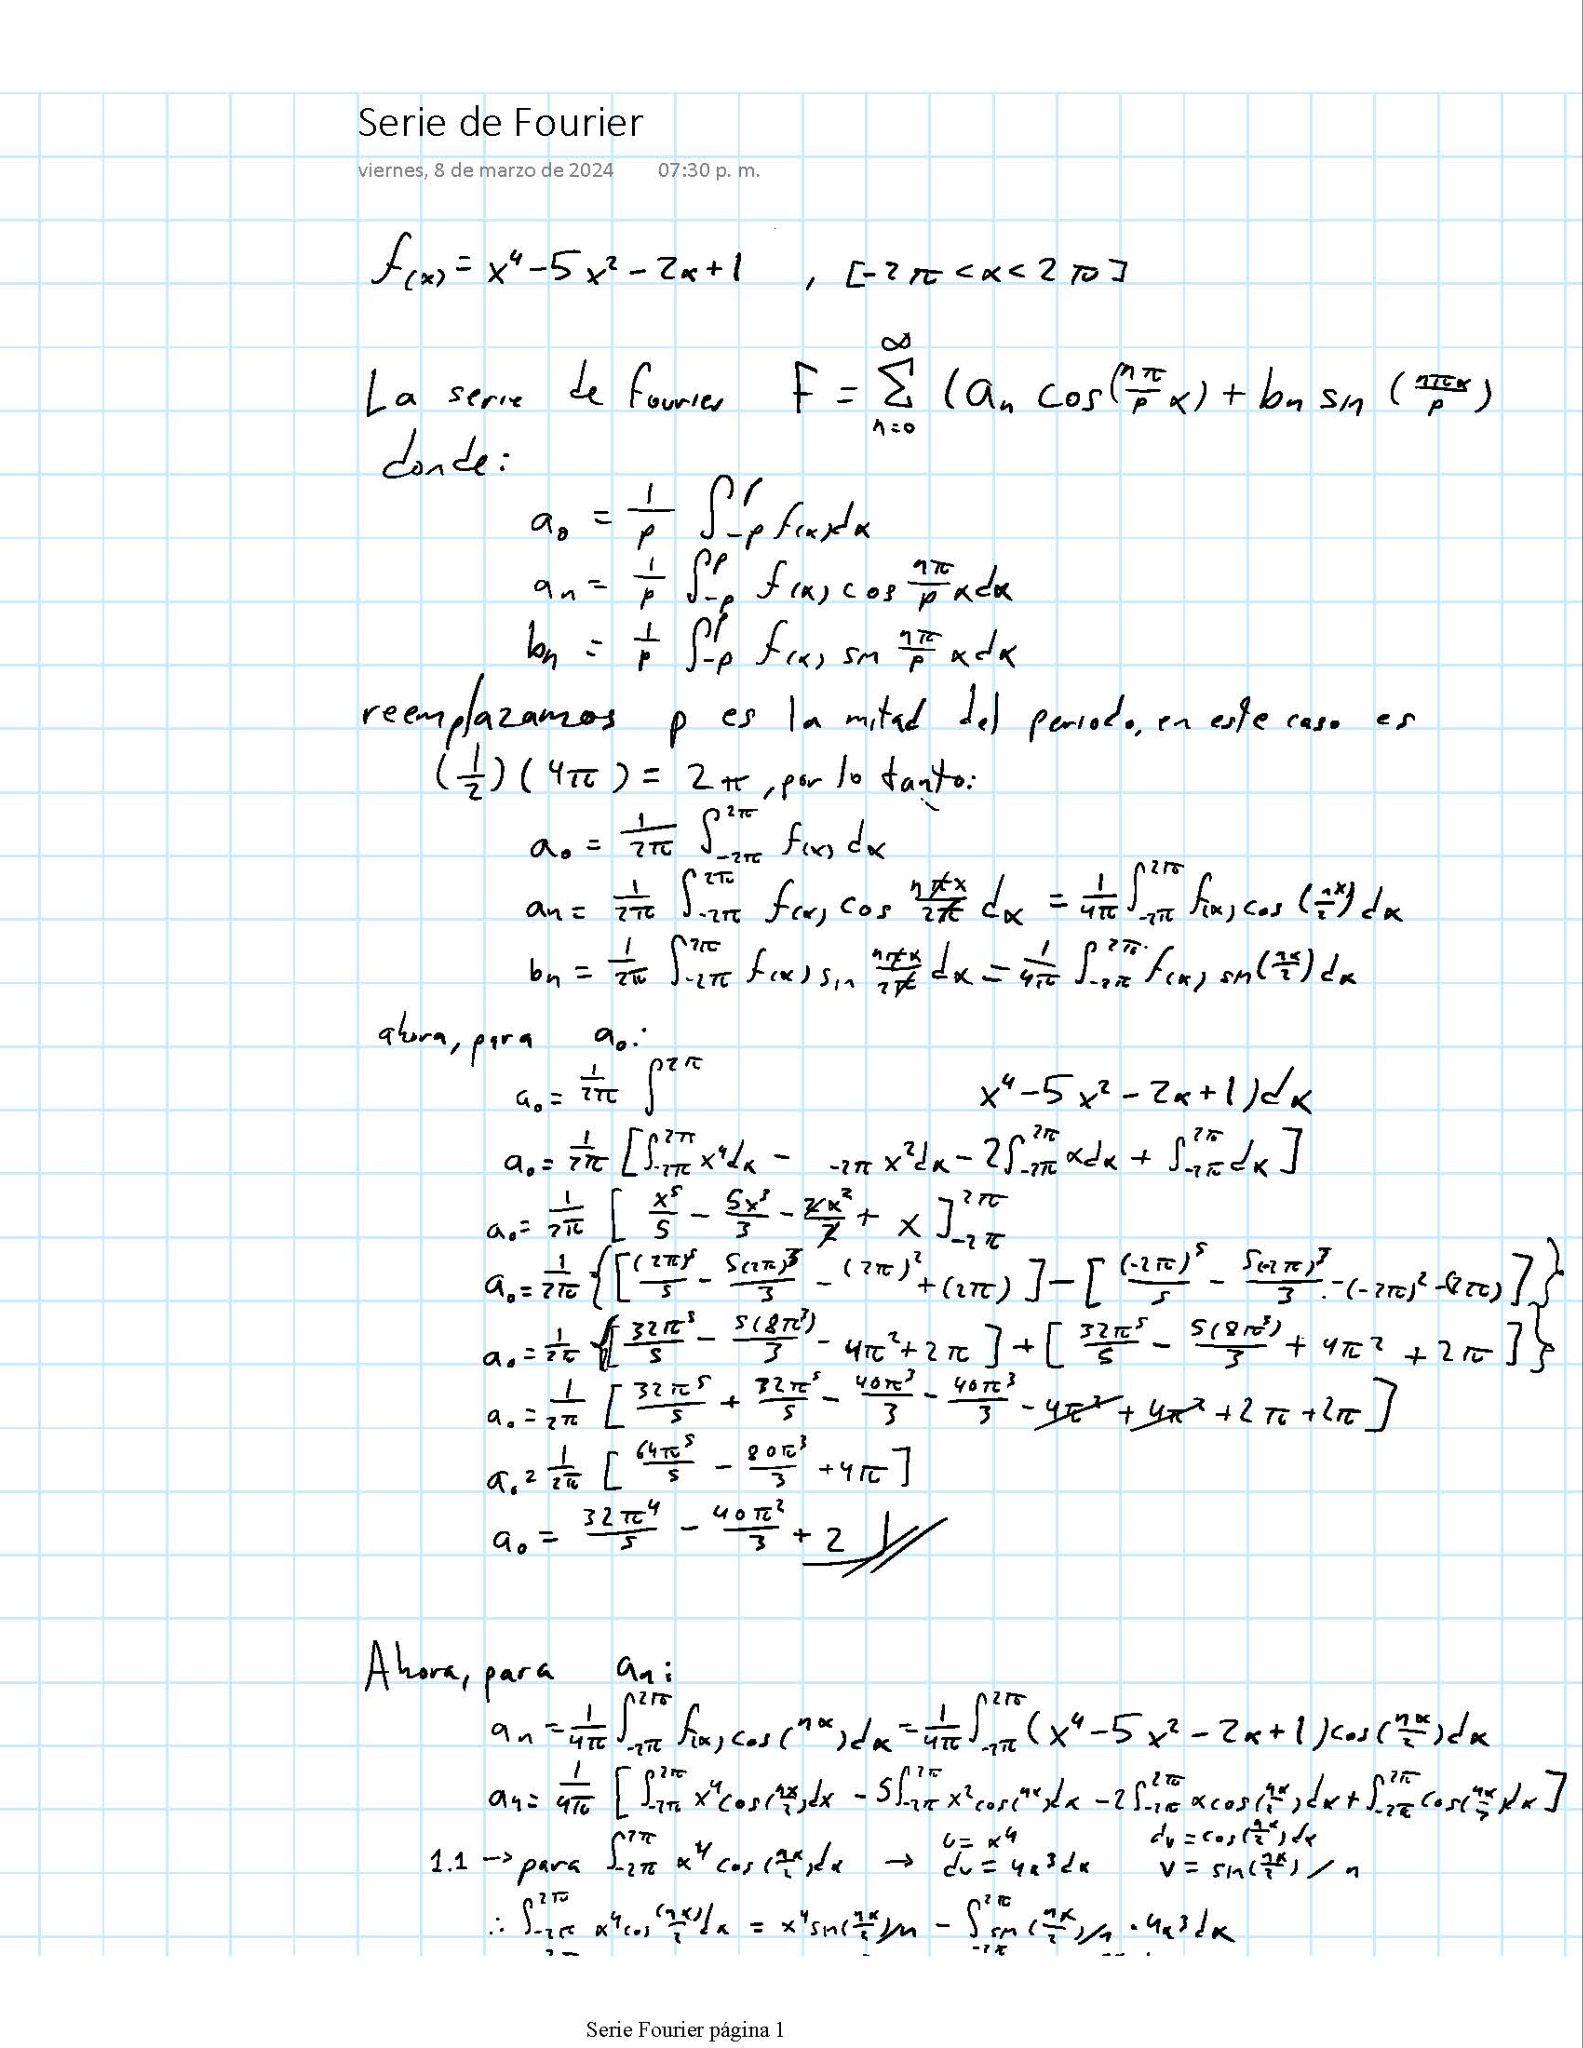
\includegraphics[width=5.93125in,height=7.67516in]{media/image59.jpg}

Imagen 1D. Procedimiento de Fourier

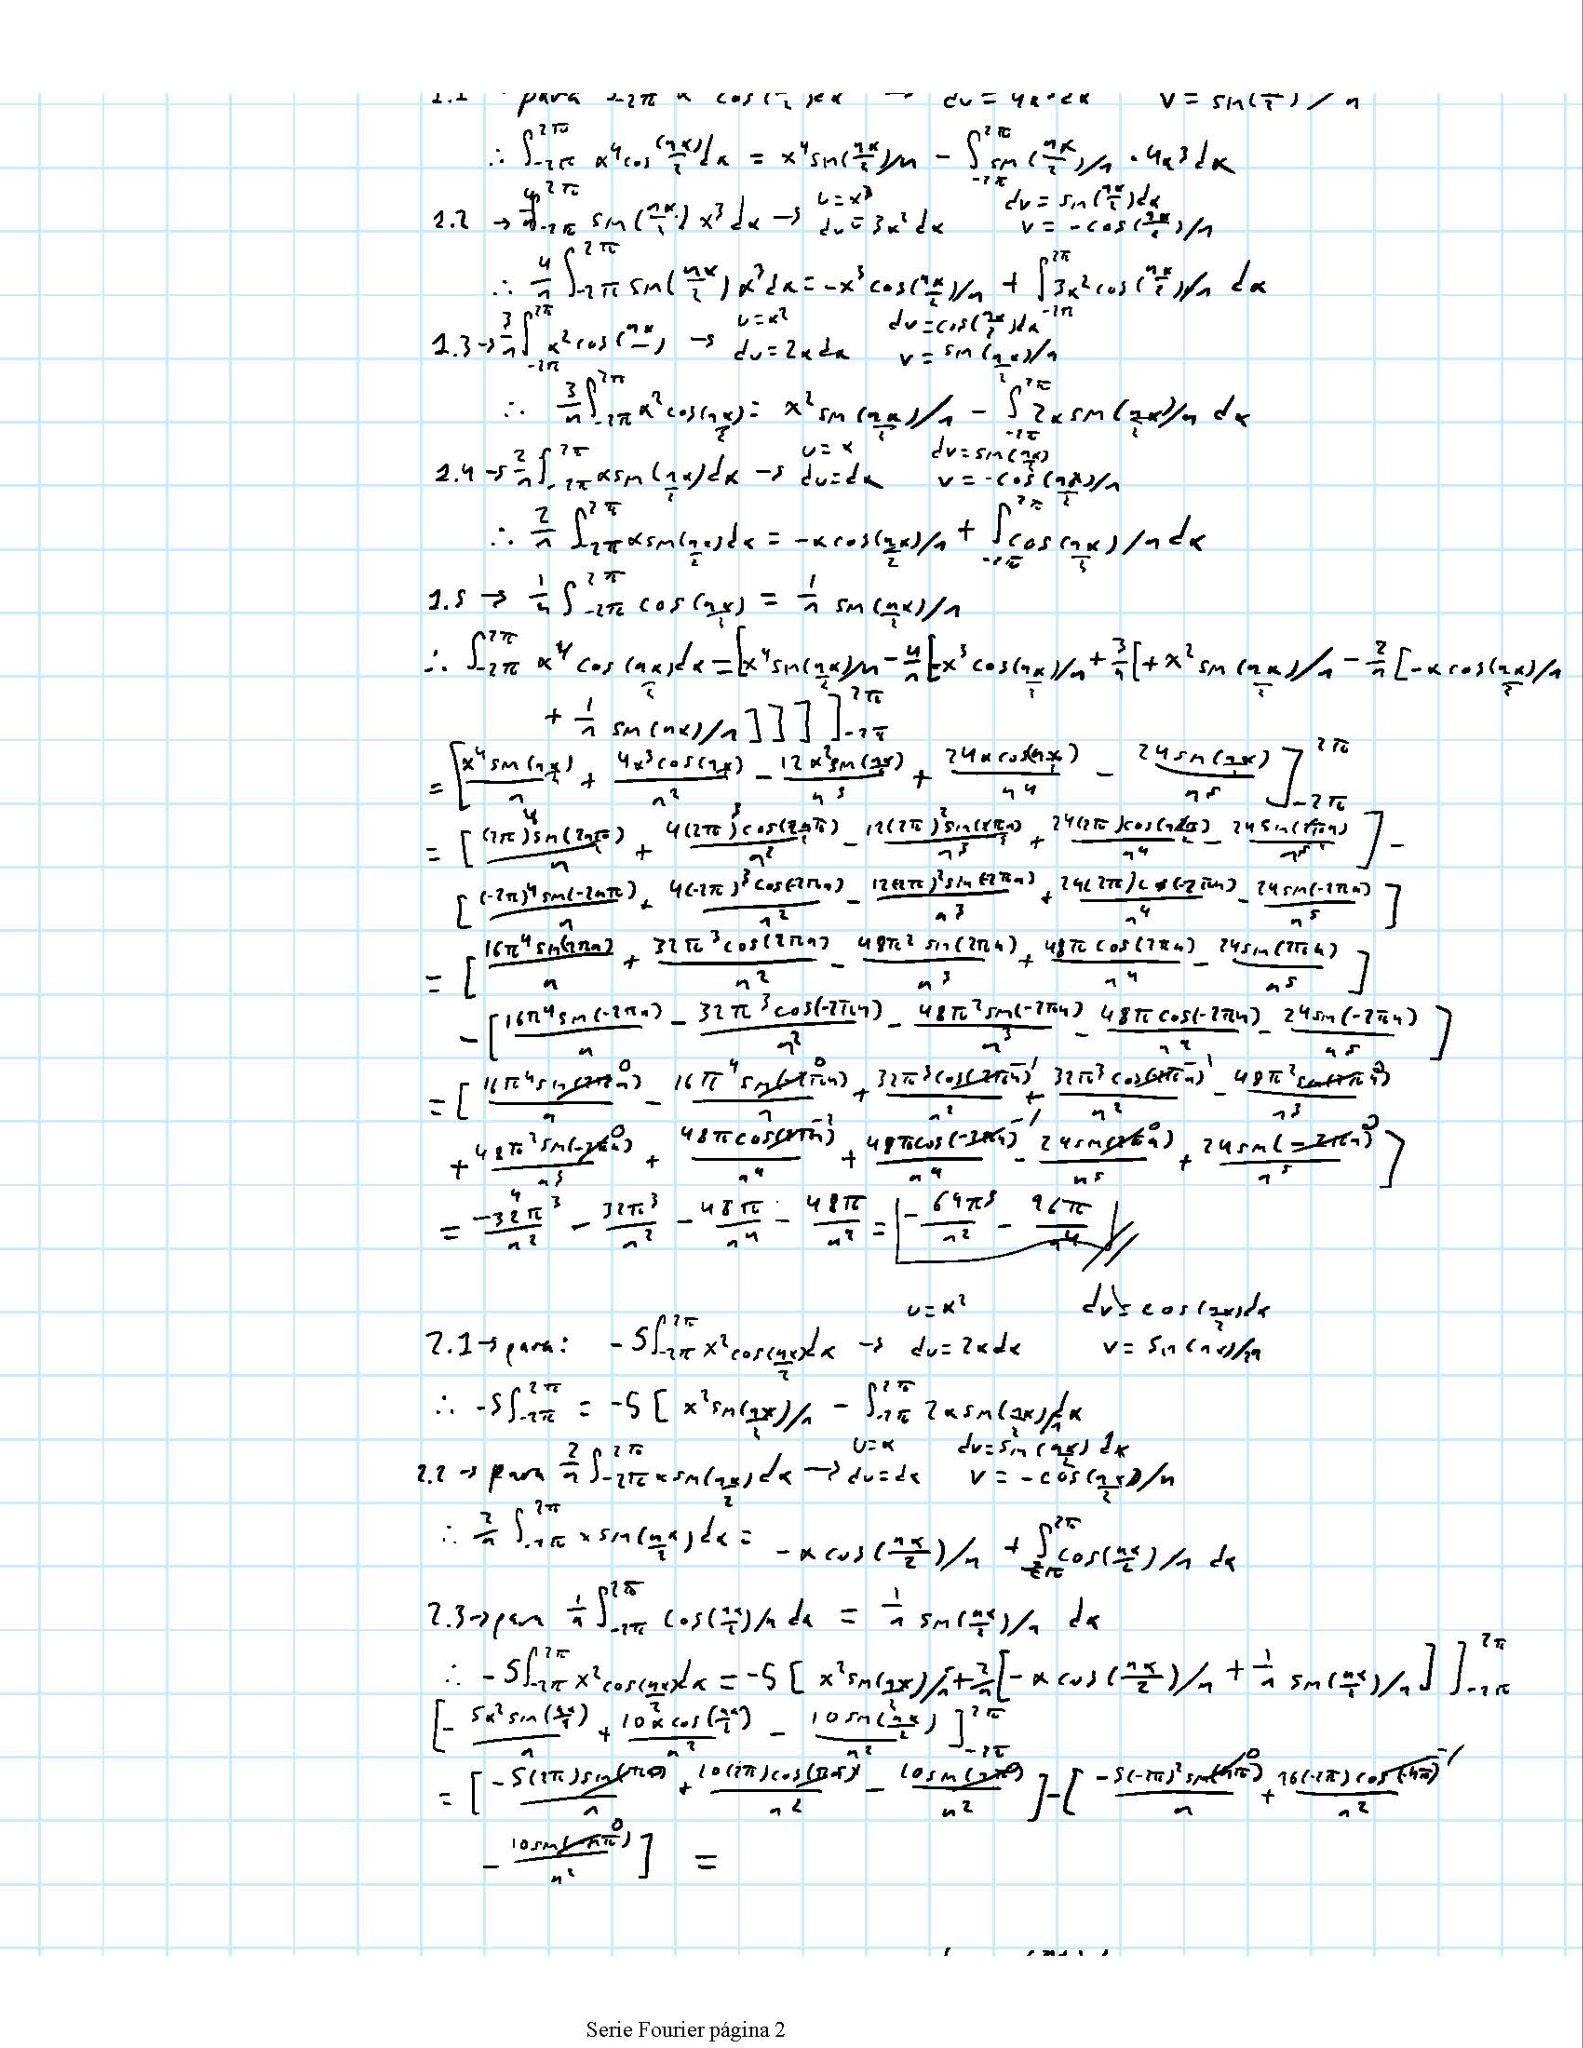
\includegraphics[width=6.26772in,height=8.11111in]{media/image56.jpg}

Imagen 2D. Procedimiento de Fourier

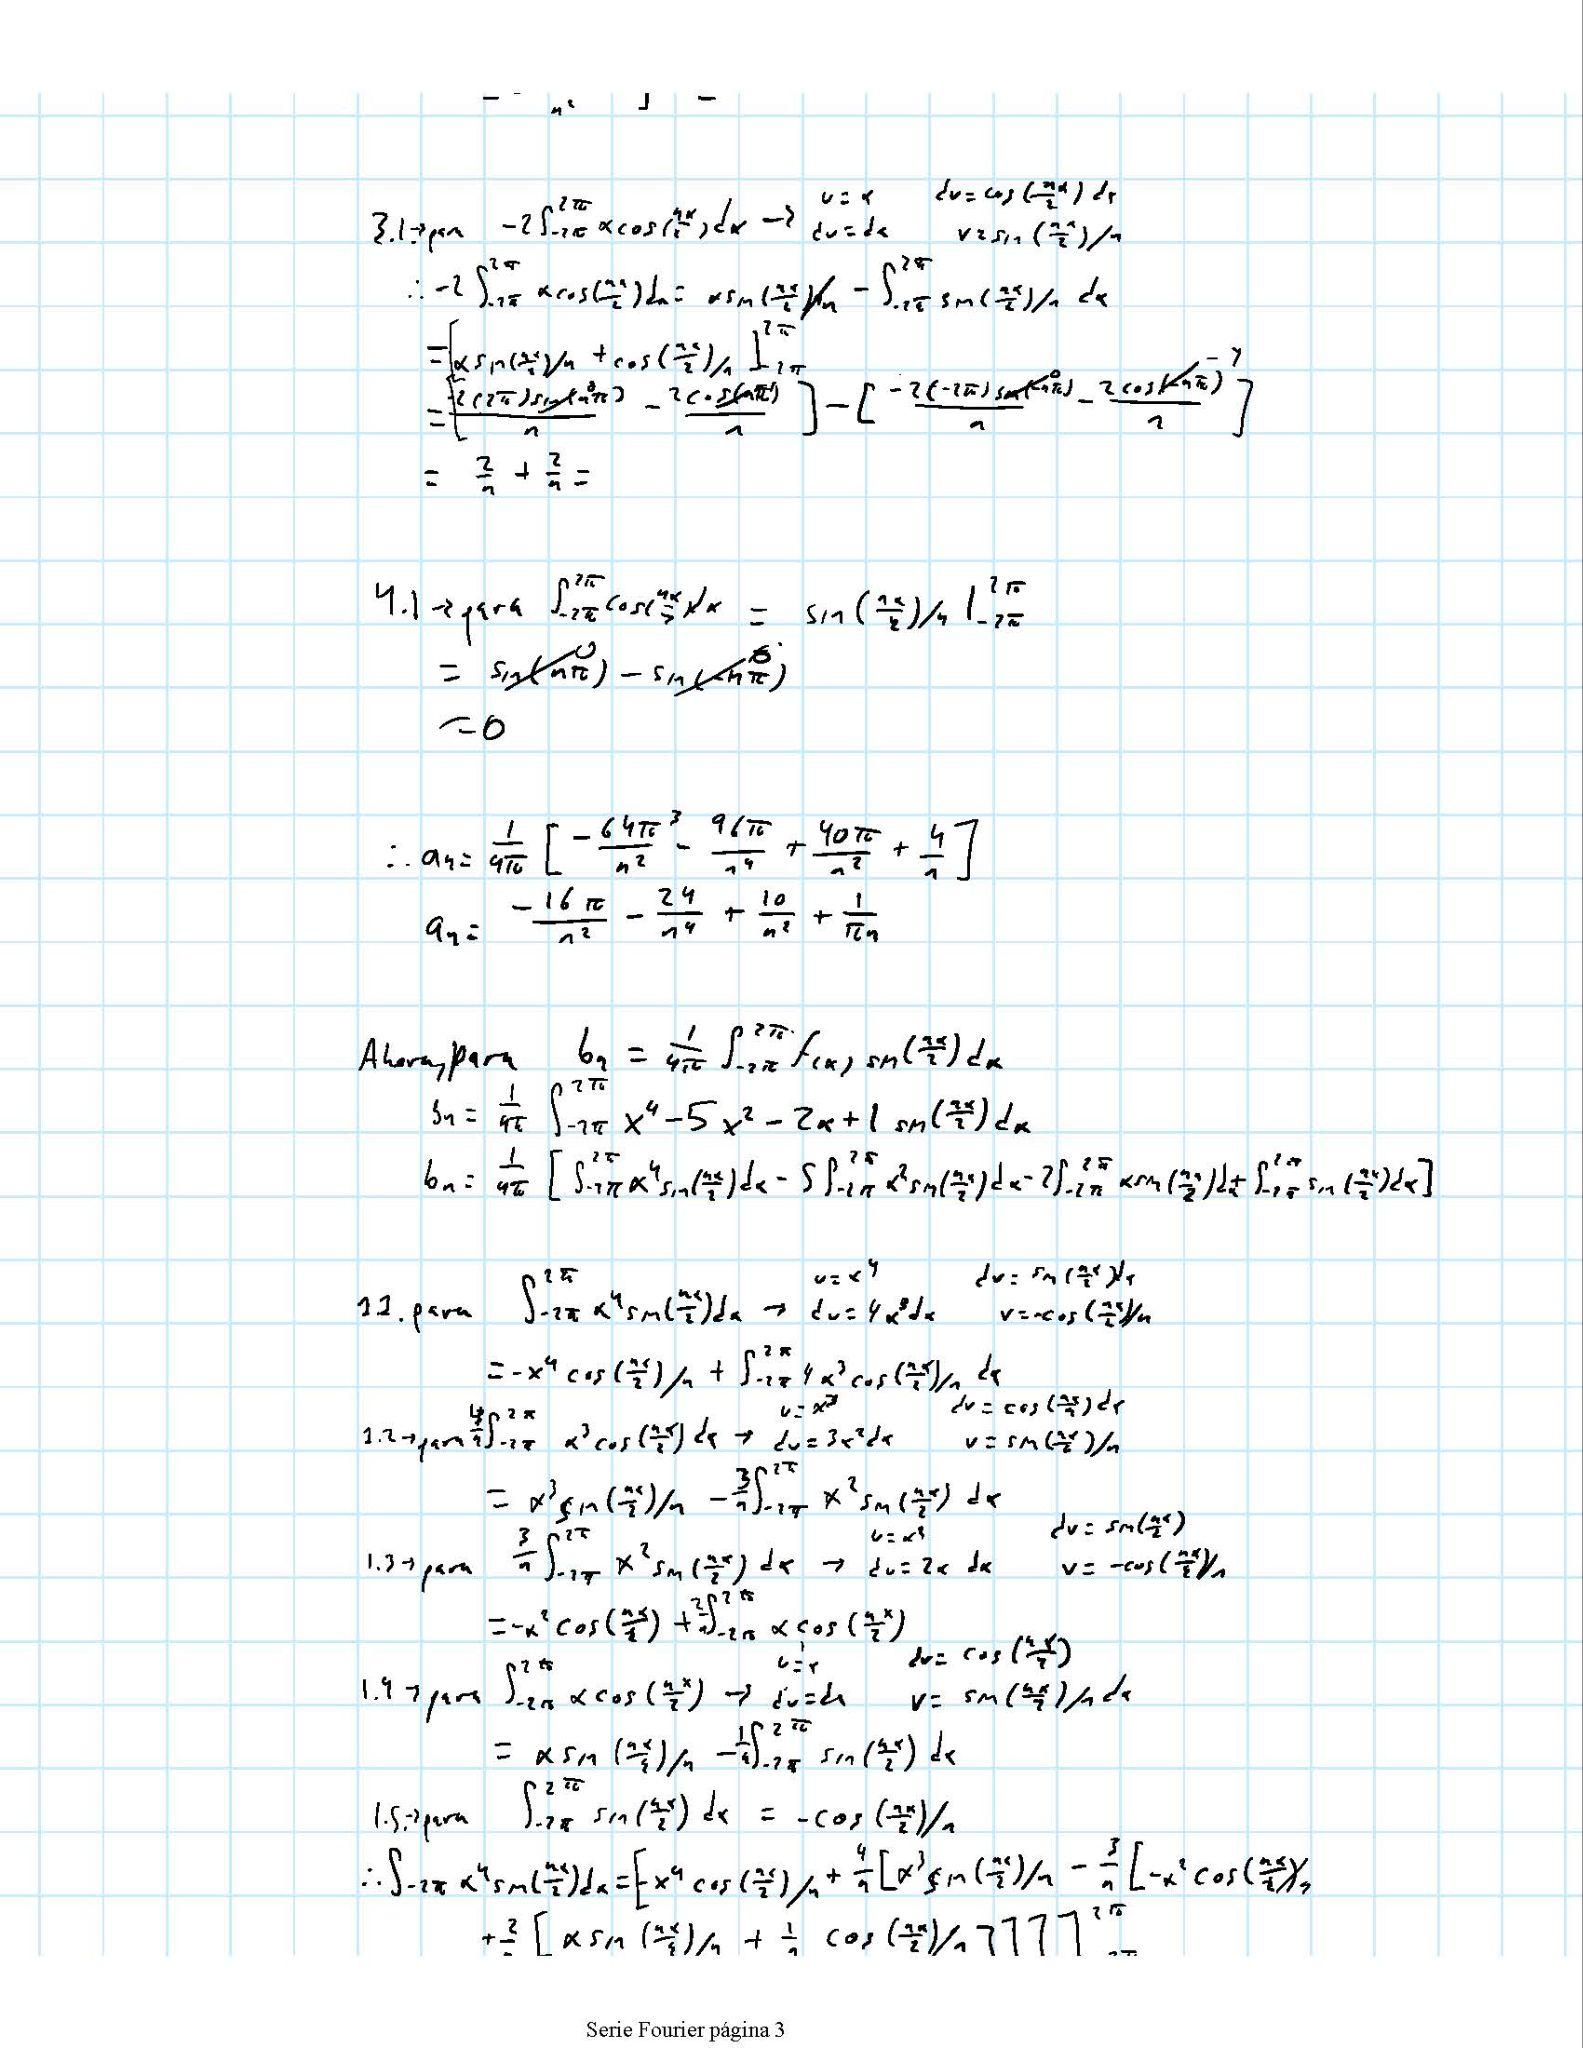
\includegraphics[width=6.26772in,height=8.11111in]{media/image55.jpg}

Imagen 3D. Procedimiento de Fourier

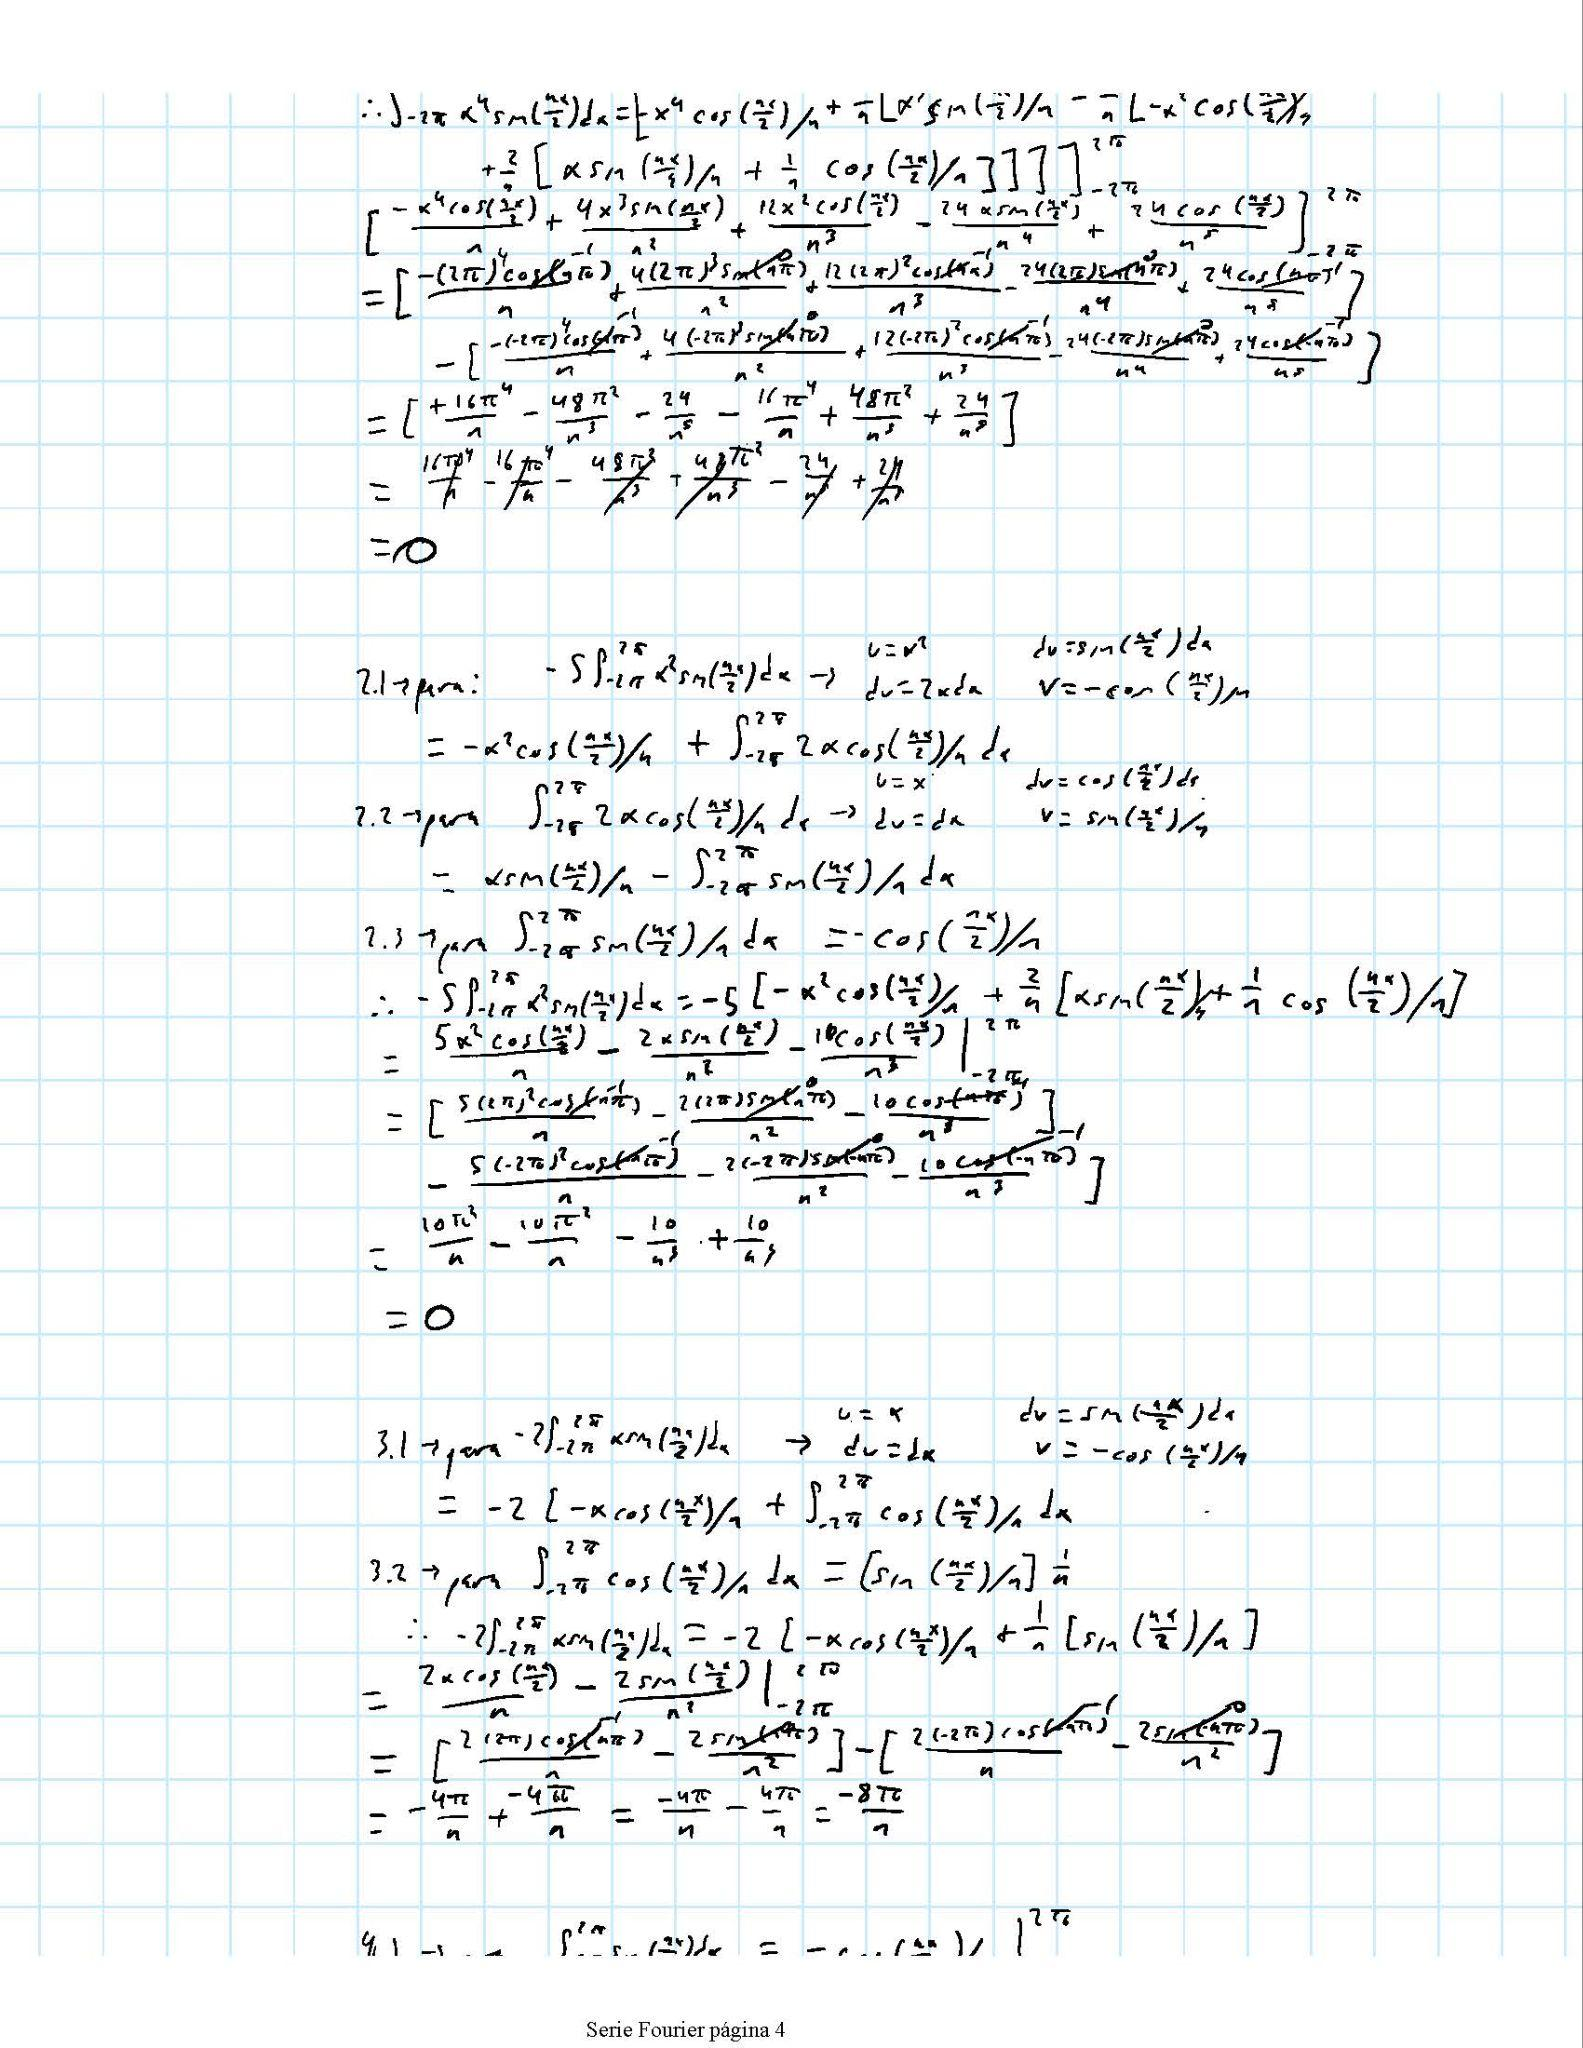
\includegraphics[width=6.26772in,height=8.11111in]{media/image57.jpg}

Imagen 4D. Procedimiento de Fourier

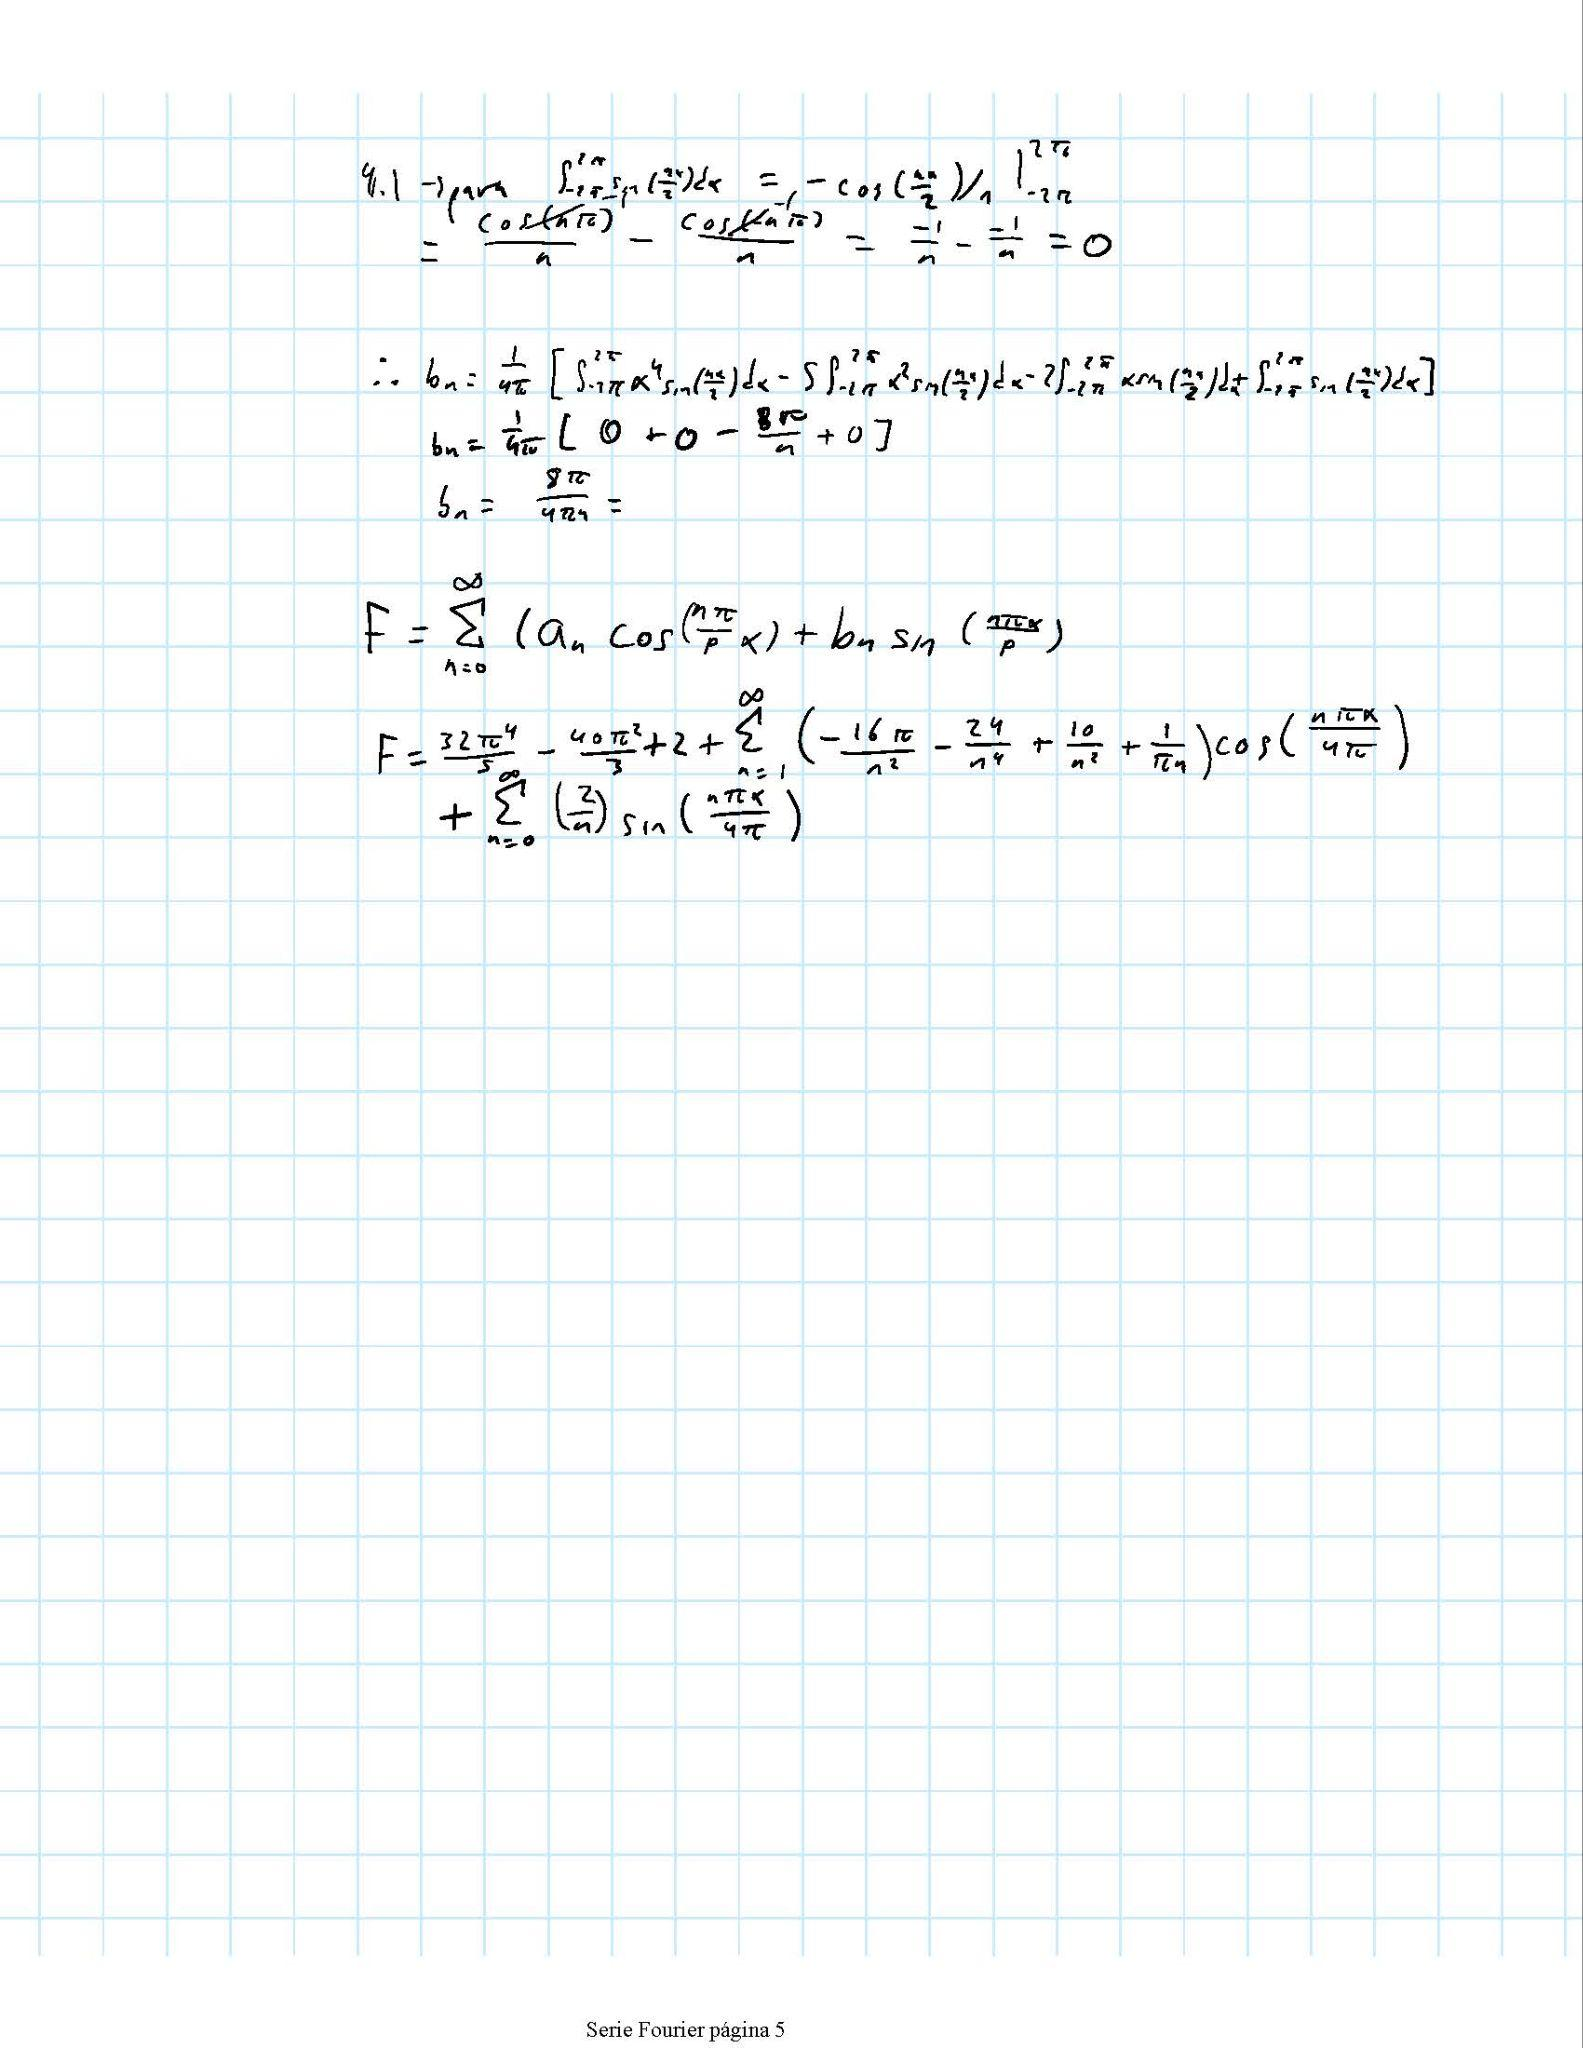
\includegraphics[width=6.26772in,height=8.11111in]{media/image58.jpg}

Imagen 5D. Procedimiento de Fourier

\section{Representación gráfica de la serie de Fourier en una hoja de cálculo}

En la siguiente figura se representa un polinomio de cuarto grado en términos de \(x\). Para graficar esta función en Excel, primero se eligen los valores de \(x\) para los cuales se desea evaluar la función. Luego, se calculan los valores correspondientes de \(y\) utilizando la expresión del polinomio. Estos pares de valores de \(x\) y \(y\) se organizan en dos columnas en Excel.

Una vez que se tienen los valores de \(x\) y \(y\), se seleccionan y se crea un gráfico de dispersión o de líneas en Excel. En este gráfico, los valores de \(x\) se colocan en el eje horizontal (eje \(x\)), mientras que los valores de \(y\) se colocan en el eje vertical (eje \(y\)).

\subsection{Figura 1. Función original}

En la figura 2, se muestran los valores de la función de acuerdo al cálculo que se efectuó.

\begin{figure}[H]
	\centering
	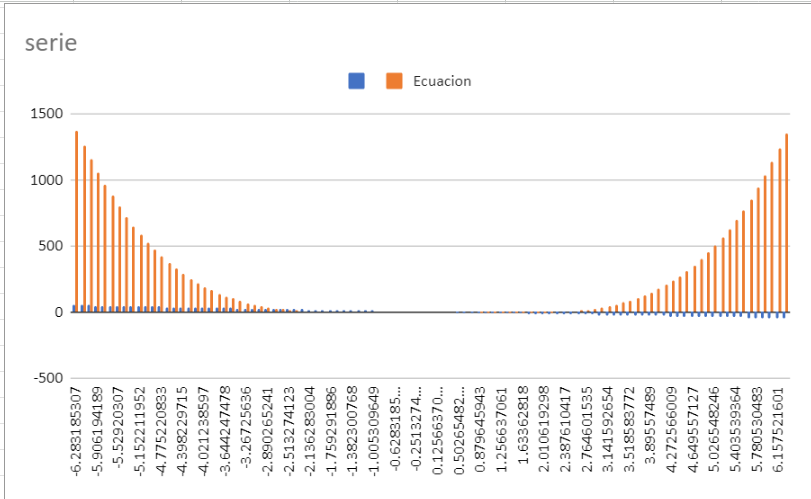
\includegraphics[width=6.26772in,height=3.44444in]{media/image10.png}
	\caption{Figura 1. Función original}
\end{figure}

\subsection{Figura 2. Función original con valores calculados}

Finalmente en la \emph{Figura 3}, podemos observar y comparar las gráficas de la función por medio de los cálculos obtenidos a mano de la serie de Fourier, viendo la forma que toman y una similitud con la original que observamos en la \emph{Figura 1}.

\begin{figure}[H]
	\centering
	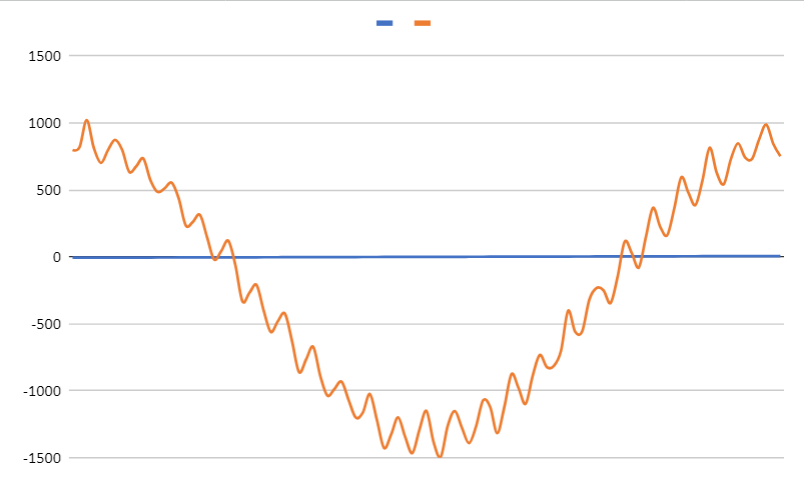
\includegraphics[width=5.10573in,height=3.08055in]{media/image16.png}
	\caption{Figura 3. Serie de Fourier aproximada en Excel}
\end{figure}

\section{Tablas}

\begin{figure}[H]
    \centering
    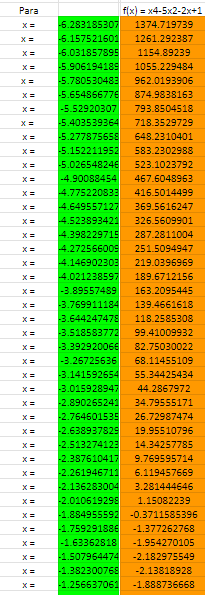
\includegraphics[width=2.13542in,height=6.19792in]{media/image23.png}
    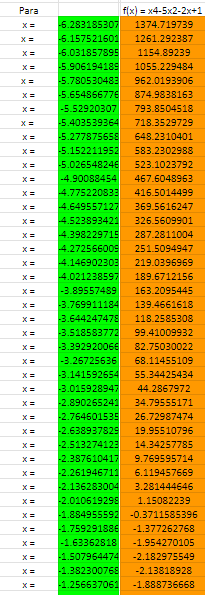
\includegraphics[width=2.13542in,height=6.19792in]{media/image23.png}    
    \caption{Función original en el rango \(-2 \pi\) a \(2 \pi\)}
\end{figure}

En la tabla 1 podemos observar los valores para la función \(\operatorname{f}(x) = x^4-5x^2-2x+1\), graficada en el intervalo \(-2 \pi\) a \(2 \pi\), para el rango de valores \(x\) , que representa el intervalo anteriormente mencionado se utilizaron 100 muestras. La columna de color verde muestra el valor de x para cada punto del intervalo, la columna naranja muestra la función evaluada en el valor. Estos valores serán utilizados para graficar la función original y así compararla con la transformada de Fourier. Cabe resaltar que contra mayor sea la cantidad de valores en que se divida el intervalo mayor será la definición que se obtenga de la función al momento de graficar.

\begin{figure}[H]
    \centering
    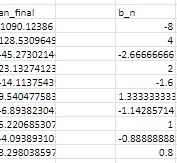
\includegraphics[width=1.84375in,height=1.69792in]{media/image1.png}
    \caption{Cálculo de \(a_n\) y \(b_n\)}        
\end{figure}

Una vez calculados los coeficientes \(a\) y \(b\) se pueden utilizar en la serie de Fourier para representar la función. Estos coeficientes representan la proyección de la función, normalizada por la longitud del periodo T.

\begin{figure}[H]
    \centering
    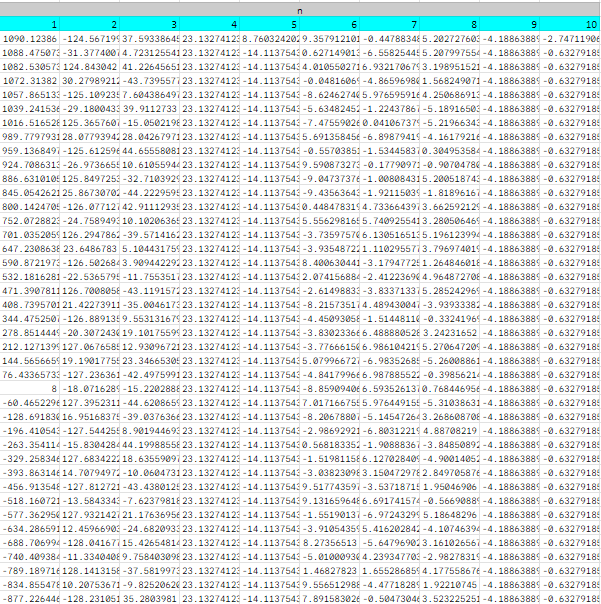
\includegraphics[width=5.5in,height=5.52745in]{media/image21.png}
    \caption{Matriz de cálculo de los coeficientes de la serie}
\end{figure}

En la tabla 3 se muestra el cálculo de los coeficientes de la serie de Fourier, cada columna (1-10), representa el cálculo de un coeficiente, los coeficientes están dados por la fórmula de series de Fourier, en donde hay que calcular \(a_n\) y \(b_n\) para cada valor de n, en este caso n siendo el intervalo 1-10, idealmente se deberían calcular todos los coeficientes, pero en este caso por las limitaciones de Excel solo se tomó una pequeña cantidad. La suma de coeficientes llevada de n=0 - n=infinito; nos daría exactamente la función que buscamos modelar, debido a que no se calculan todos en esta práctica veremos solamente una aproximación a la función original. Estos valores posteriormente serán utilizados para graficarlos y comparar la función original con la transformada de Fourier.

\begin{figure}[H]
    \centering
    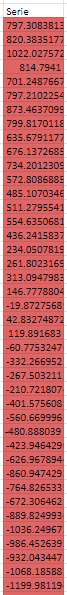
\includegraphics[width=0.69792in,height=6.19792in]{media/image28.png}
    \caption{Cálculo de la serie}
\end{figure}
En la Tabla 4 se muestran los resultados de los cálculos realizados que toman los valores de la serie de Fourier, se obtienen mediante la suma de los coeficientes previamente calculados, estos son utilizados para representar una función periódica como una suma de senos y cosenos.

\section{Programación de la serie de Fourier en lenguaje C}

\subsection{Implementación de código}

\begin{enumerate} 
	\def\labelenumi{\arabic{enumi}.} 
	\item Se incluyen las bibliotecas necesarias para su funcionamiento y se define el valor de PI y las constantes necesarias, finalmente
	
	\begin{figure}[H]
		\centering
		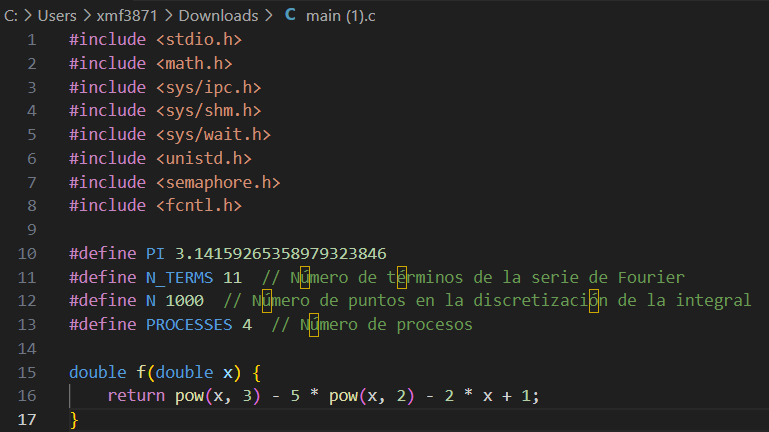
\includegraphics[width=5.55729in,height=3.12944in]{media/image18.png}
		\caption{Código}
	\end{figure}
	
	\item La función \emph{calculate coefficients} se encarga de calcular los coeficientes de la serie de Fourier para un rango de términos n específico. Utiliza una técnica de sincronización con semáforos para garantizar que cada proceso realice sus cálculos de manera ordenada.
	
	\begin{figure}[H]
		\centering
		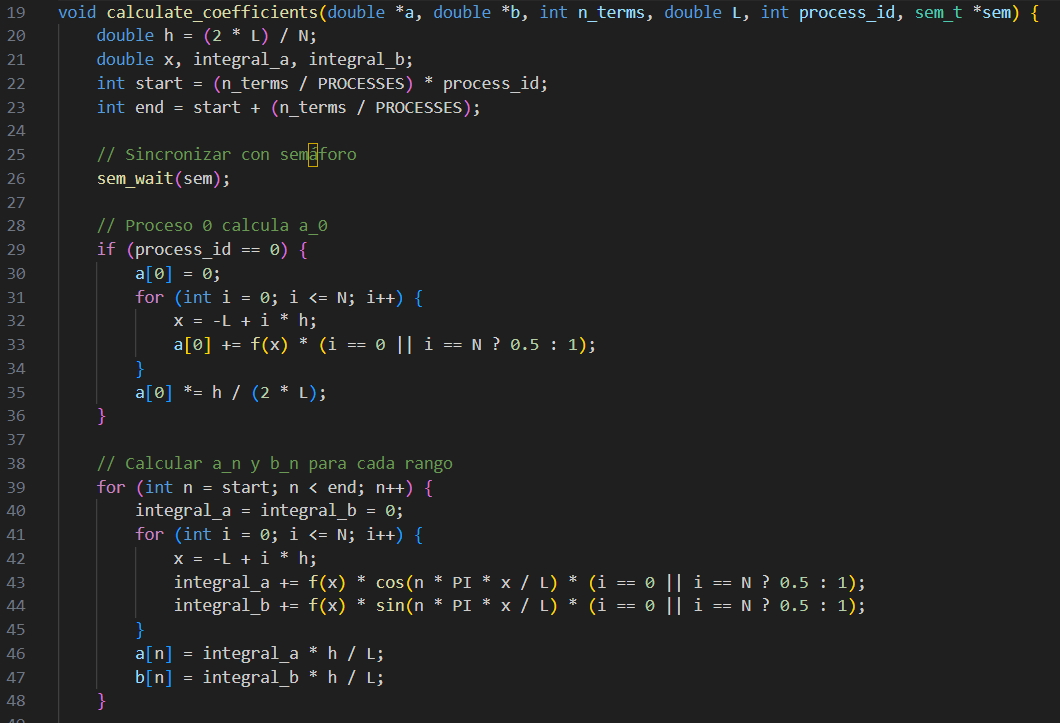
\includegraphics[width=5.64741in,height=3.85562in]{media/image39.png}
		\caption{Función calculate coefficients}
	\end{figure}
	
	\item La función \emph{fourier\_approximation} calcula la aproximación de la función original utilizando los coeficientes de la serie de Fourier.
	
	\begin{figure}[H]
		\centering
		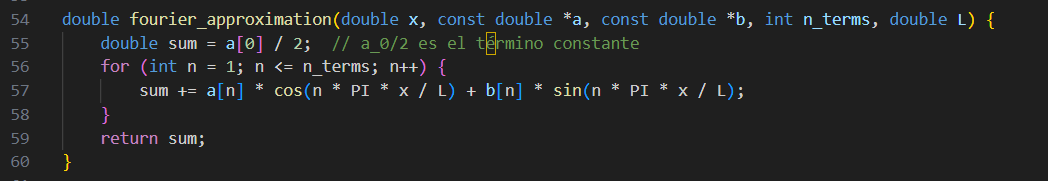
\includegraphics[width=6.26772in,height=1.08333in]{media/image11.png}
		\caption{Función fourier approximation}
	\end{figure}
	
	\item La función \emph{export\_to\_csv} exporta los resultados a un archivo CSV que contiene los valores de x, la función original y la aproximación de la serie de Fourier y\_fourier.
	
	\begin{figure}[H]
		\centering
		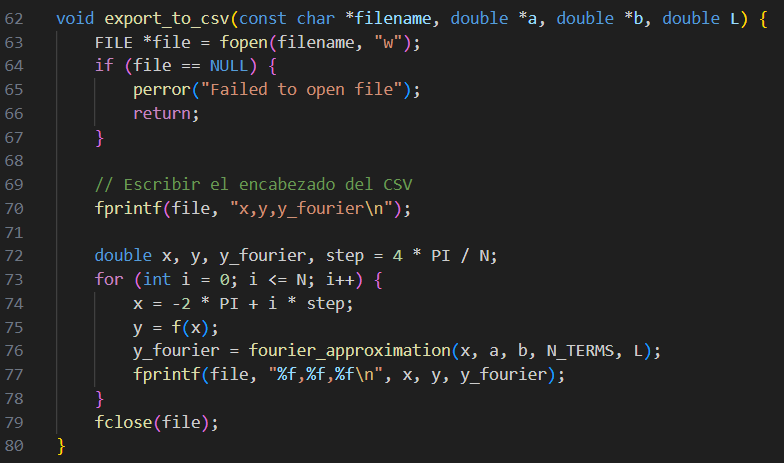
\includegraphics[width=5.02604in,height=2.61756in]{media/image50.png}
		\caption{Función export\_to\_csv}
	\end{figure}
	
	\item En la función main, se crea un segmento de memoria compartida para almacenar los coeficientes a y b, se crea un semáforo para la sincronización entre procesos y se generan varios procesos hijos para calcular los coeficientes de la serie de Fourier en paralelo. Después de que todos los procesos hayan terminado de calcular los coeficientes, se exportan los resultados a un archivo CSV y se liberan los recursos utilizados.
	
	\begin{figure}[H]
		\centering
		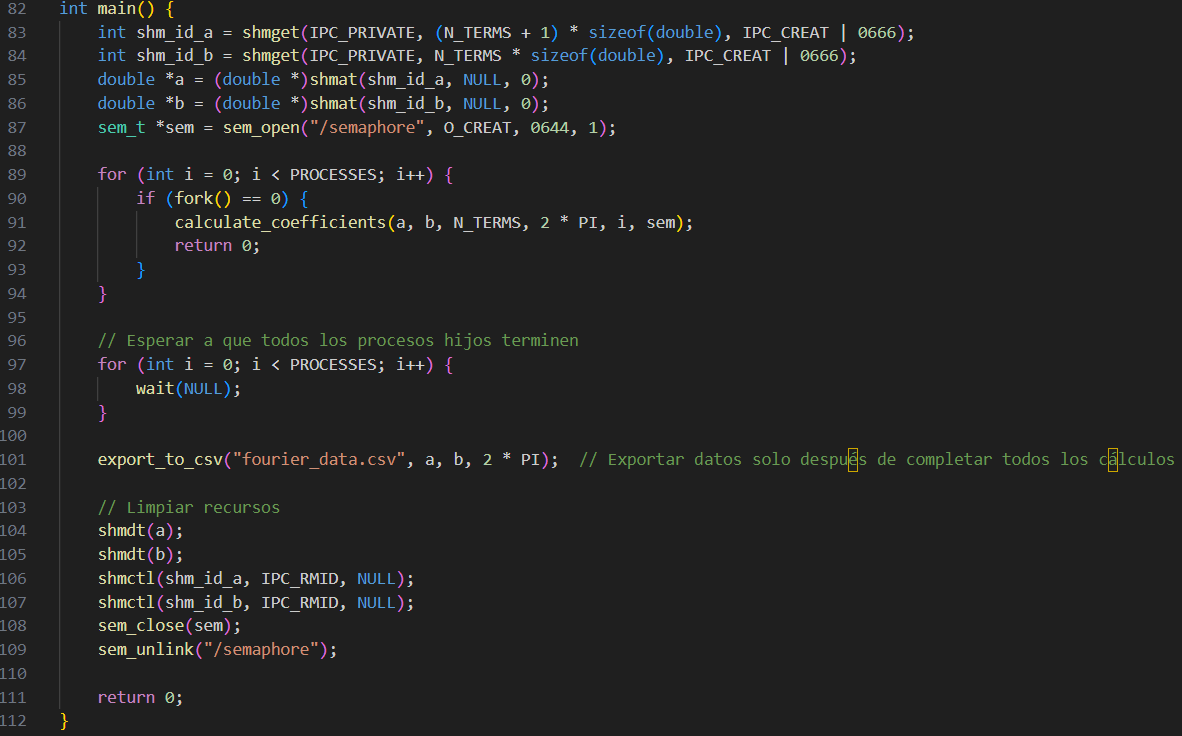
\includegraphics[width=6.26772in,height=3.90278in]{media/image7.png}
		\caption{Función main}
	\end{figure}
	
\end{enumerate}

\subsection{Ejecución del código}

\begin{enumerate} 
	\def\labelenumi{\arabic{enumi}.} 
	\item Ejecución de código en linux
	
	\begin{figure}[H]
		\centering
		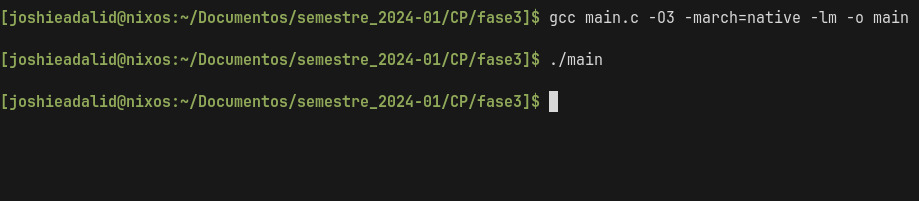
\includegraphics[width=6.26772in,height=1.375in]{media/image29.png}
		\caption{Ejecución en Linux}
	\end{figure}
	
	\item Visualización del archivo generado. Para cada x, su evaluación en la función a aproximar, y su aproximación de la serie de Fourier.
	
	\begin{figure}[H]
		\centering
		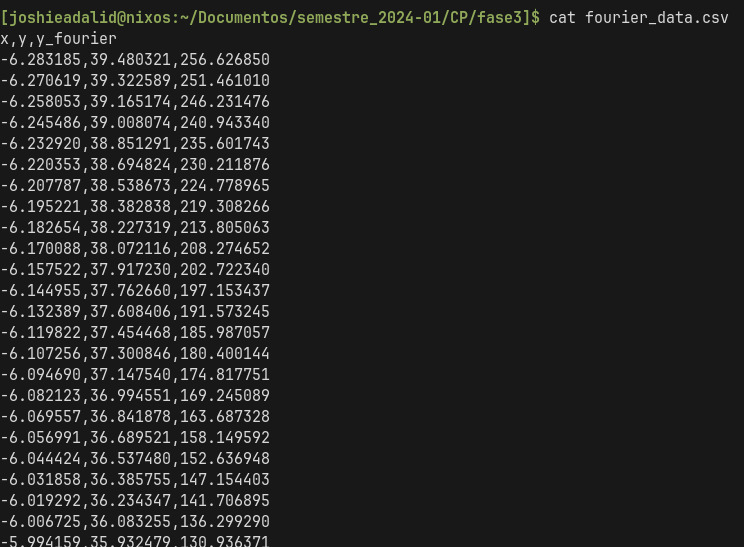
\includegraphics[width=5.16146in,height=3.79822in]{media/image37.png}
		\caption{Aproximación para la serie de Fourier}
	\end{figure}
	
	\begin{figure}[H]
		\centering
		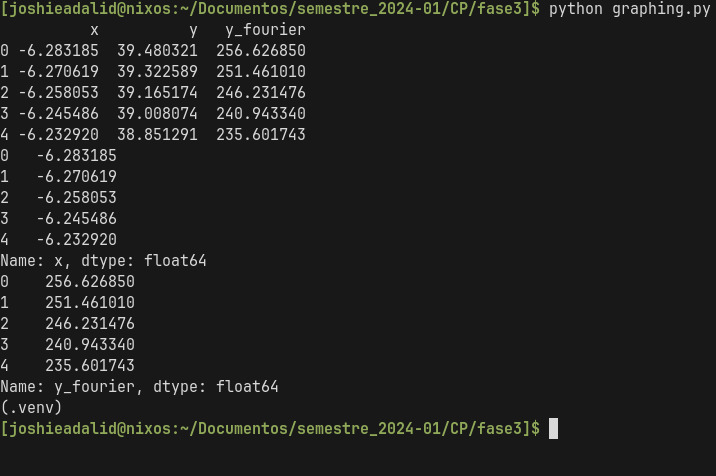
\includegraphics[width=5.16146in,height=3.42309in]{media/image25.png}
		\caption{Aproximación para la serie de Fourier}
	\end{figure}
	
	\item Gráfica generada
	
	\begin{figure}[H]
		\centering
		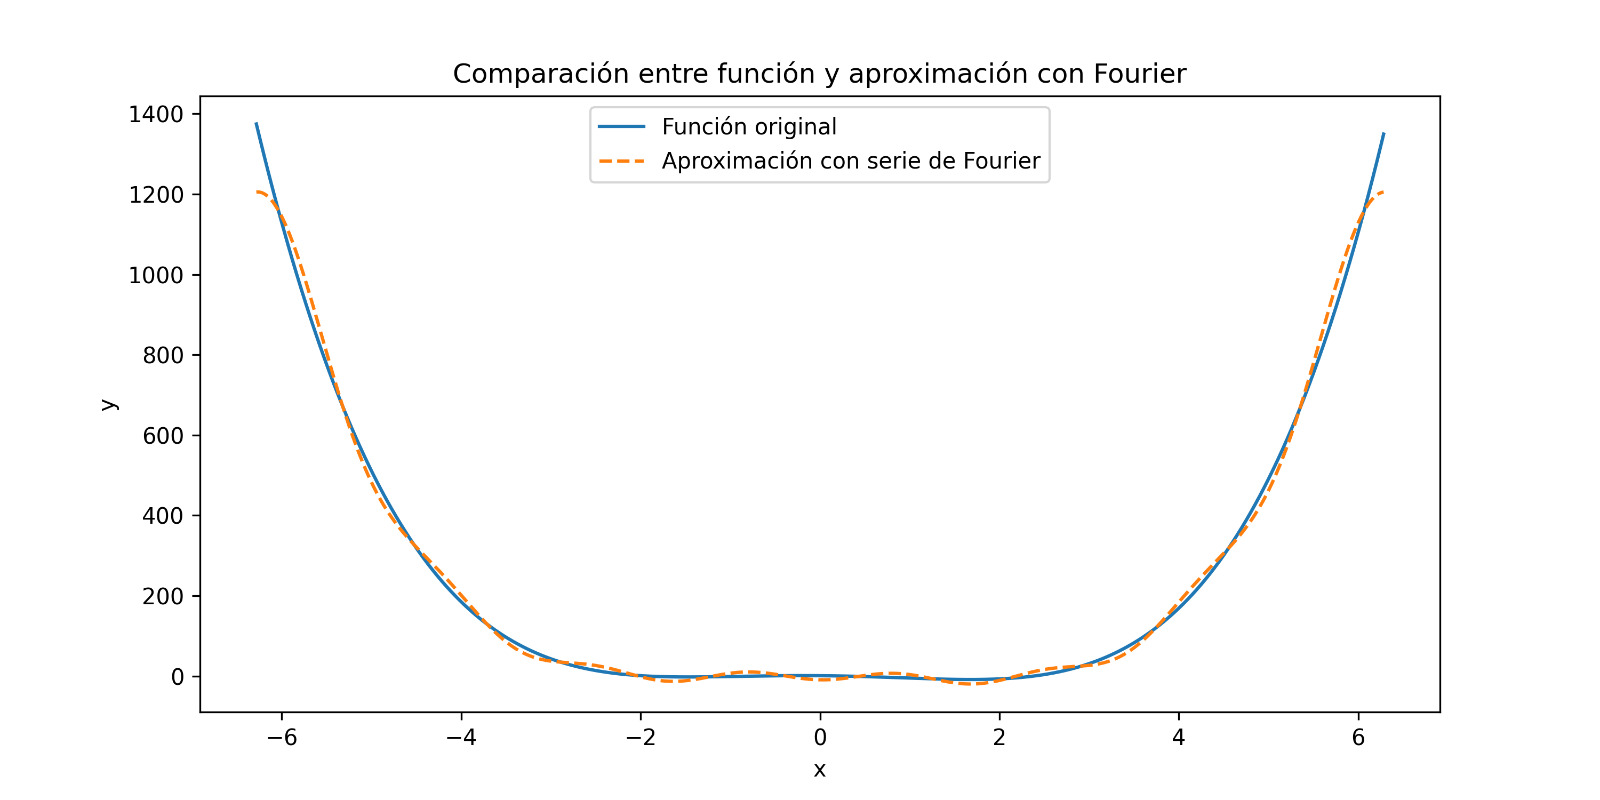
\includegraphics[width=6.26772in,height=3.13889in]{media/image12.png}
		\caption{Gráfica original y aproximación de Fourier en C}
	\end{figure}
	
\end{enumerate}

\subsection{Implementación de código con hilos}

En este apartado se mostrará y explicará el código implementado ahora con hilos en lugar de memoria compartida y semáforos.

\begin{enumerate} 
	\def\labelenumi{\arabic{enumi}.} 
	\item En primer lugar, se incluyen las bibliotecas necesarias para utilizar las funciones básicas y las funciones de hilos como se muestran en la imagen 13, así como definir unas constantes que nos ayudarán a ejecutar el programa con hilos.
	
	\begin{figure}[H]
		\centering
		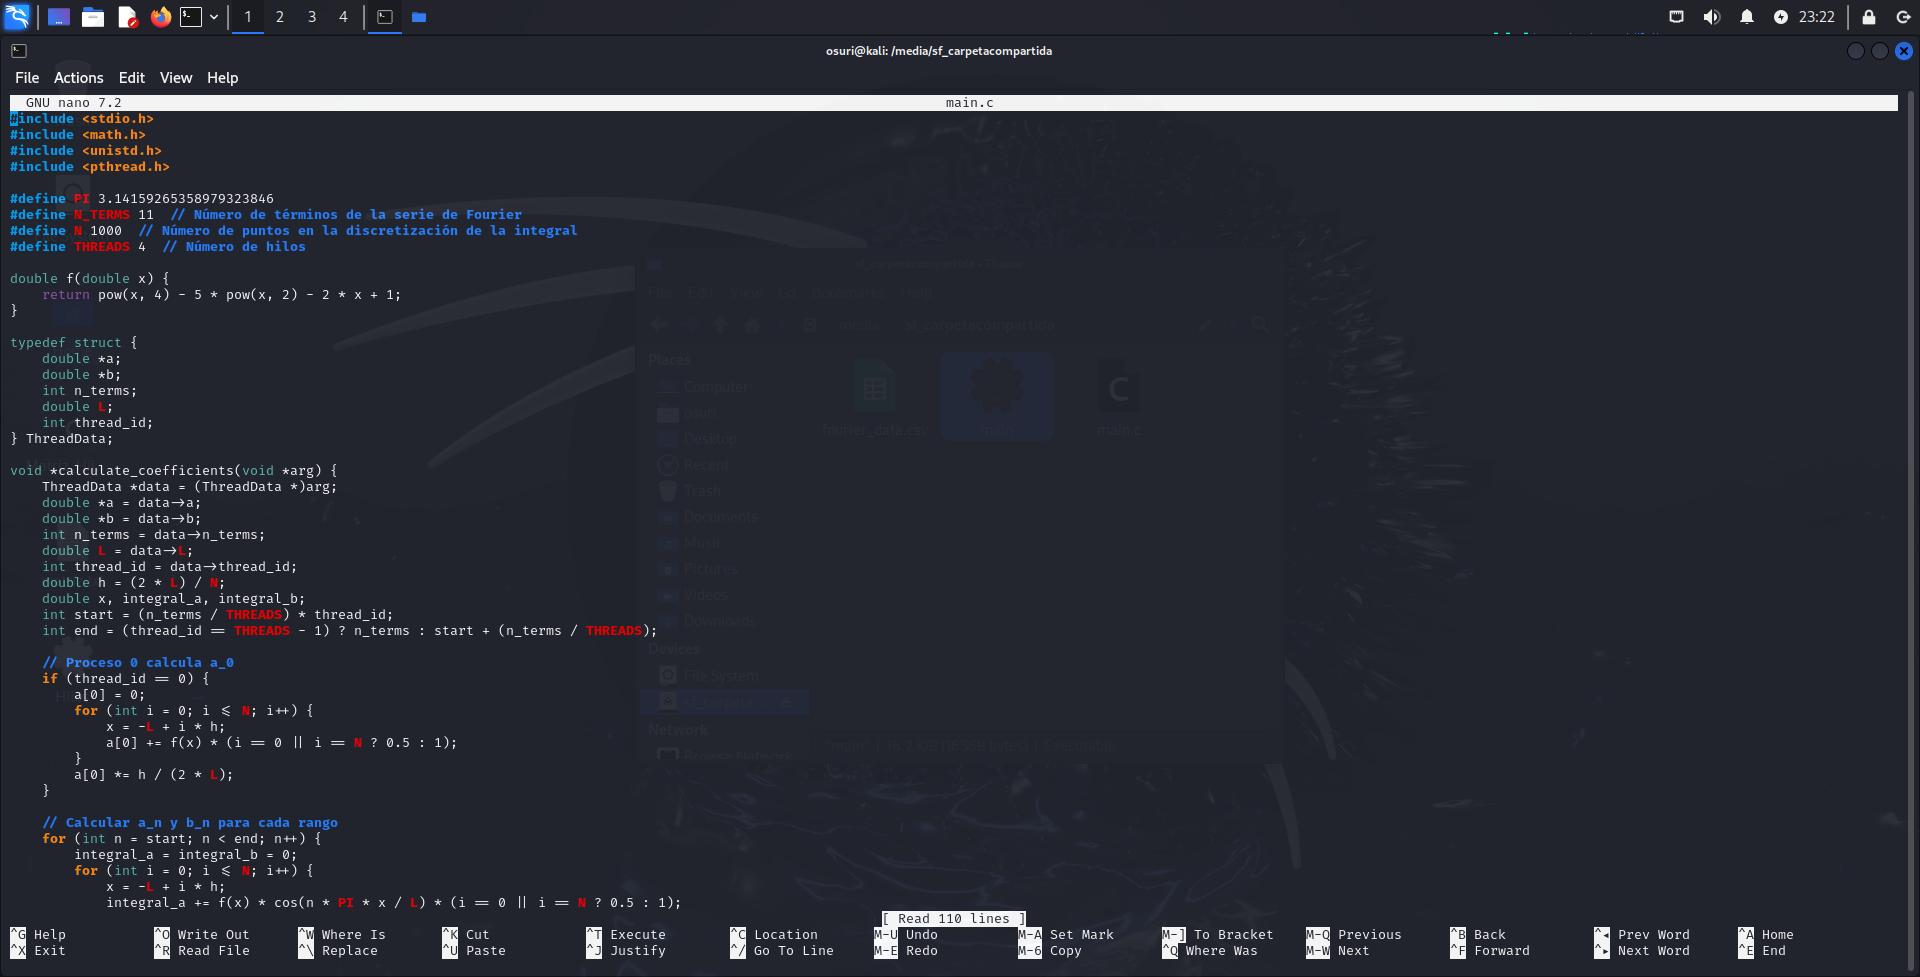
\includegraphics[width=4.53385in,height=1.24967in]{media/image4.png}
		\caption{Código 1. Fuente: Autoría propia}
	\end{figure}
	
	\item En la imagen 14 se define la estructura básica de la serie original y se crea la estructura de un hilo para que tenga los datos de la ecuación de la serie, así como los valores que debe de calcular, para almacenar múltiples tipos de datos y no entre en conflicto.
	
	\begin{figure}[H]
		\centering
		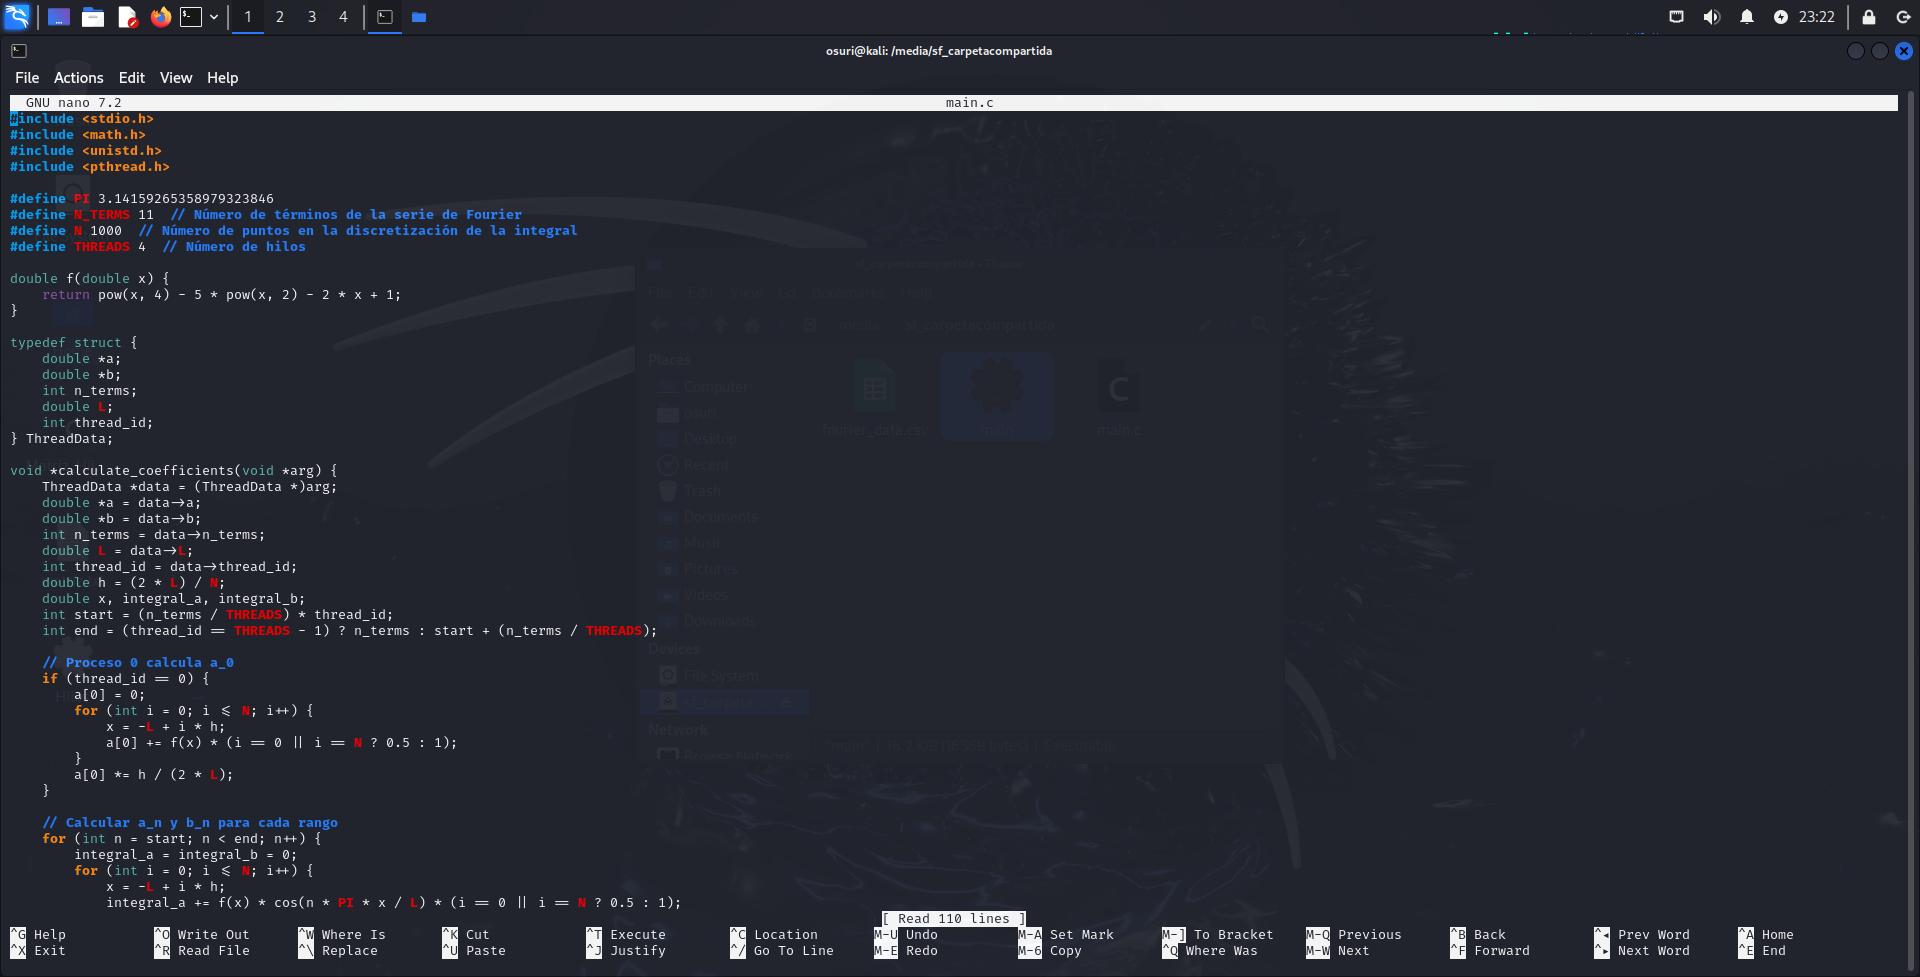
\includegraphics[width=3.15in,height=1.54172in]{media/image4.png}
		\caption{Código 2. Fuente: Autoría propia}
	\end{figure}
	
	\item En la imagen 15, se define una función para resolver la serie de Fourier por medio de hilos, se divide la información para que pueda ser ejecutada miles de veces, y se crean los hilos separados para resolver los cálculos. Se pone separado el cálculo de a0 porque sólo se calcula una vez, mientras que an y bn deben ser calculados tantas veces como "n" existan.
	
	\begin{figure}[H]
		\centering
		\includegraphics[width=3.00416in,height=2.52623in]{media/image17.png}
		\caption{Código 3. Fuente: Autoría propia}
	\end{figure}
	
	\item En la imagen 16 se crea una función de aproximación con la serie original para comparar los valores.
	
	\begin{figure}[H]
		\centering
		\includegraphics[width=4.31145in,height=0.71292in]{media/image27.png}
		\caption{Código 4. Fuente: Autoría propia}
	\end{figure}
	
	\item En la imagen 17, se crea la función para exportar los cálculos exitosos a un archivo CSV para poder guardarlos y consultarlos.
	
	\begin{figure}[H]
		\centering
		\includegraphics[width=4.19531in,height=2.2036in]{media/image27.png}
		\caption{Código 5. Fuente: Autoría propia}
	\end{figure}
	
	\item En la imagen 18, se puede observar el programa main, donde se ejecuta el proceso principal, se crean los hilos de acuerdo a la cantidad de veces que se ejecutará la secuencia, en este caso 1000, se utilizará la estructura del hilo definida con anterioridad para ejecutar los hilos, y finalmente se utilizará la función para exportar a CSV para guardar los datos.
	
	\begin{figure}[H]
		\centering
		\includegraphics[width=3.82031in,height=2.4068in]{media/image5.png}
		\caption{Código 6. Fuente: Autoría propia}
	\end{figure}
	
\end{enumerate}

\subsection{Ejecución del código con hilos}

\begin{enumerate} 
	\def\labelenumi{\arabic{enumi}.} 
	\item Compilación y ejecución (ver imagen 19).
	
	\begin{figure}[H]
		\centering
		\includegraphics[width=3.46875in,height=0.8384in]{media/image36.png}
		\caption{Compilación y ejecución. Fuente: Autoría propia}
	\end{figure}
	
	\item Visualización menor de datos, solo se utilizan ciertos datos para no saturar el documento (ver imagen 20).
	
	\begin{figure}[H]
		\centering
		\includegraphics[width=2.29583in,height=4.29598in]{media/image35.png}
		\caption{Datos de archivo CSV. Fuente: Autoría propia}
	\end{figure}
	
	\item Gráfica generada por este conjunto de datos (ver figura 5)
	
	\begin{figure}[H]
		\centering
		\includegraphics[width=6.26772in,height=3.13889in]{media/image30.png}
		\caption{Gráfica generada. Fuente: Autoría propia}
	\end{figure}
	
\end{enumerate}

\subsection{Ejecución del código con MPI}
\begin{figure}[H]
	\includegraphics[width=0.8\textwidth]{media/mpi_grafica.jpeg}
	\caption{Comparación de la función original contra la aproximación de la serie de Fourier, calculado con la tecnología de MPI}
\end{figure}

\begin{figure}[H]
	\includegraphics[width=0.8\textwidth]{media/mpi_codigo_1.png}
	\caption{Fragmento del código fuente en C para MPI. Parte 1 de 4.}
\end{figure}
\begin{figure}[H]
	\includegraphics[width=0.8\textwidth]{media/mpi_codigo_2.png}
	\caption{Fragmento del código fuente en C para MPI. Parte 2 de 4.}
\end{figure}
\begin{figure}[H]
	\includegraphics[width=0.8\textwidth]{media/mpi_codigo_3.png}
	\caption{Fragmento del código fuente en C para MPI. Parte 3 de 4.}
\end{figure}
\begin{figure}[H]
	\includegraphics[width=0.8\textwidth]{media/mpi_codigo_4.png}
	\caption{Fragmento del código fuente en C para MPI. Parte 4 de 4.}
\end{figure}
\section{Conclusiones}
\subsection{Juárez Botello Josué Adalid}

La verdad es que intentar resolver la serie de Fourier para una función como \(f(x)=x^4-5x^2-2x+1\) fue algo que al principio me parecía súper complicado. Al principio, ni siquiera estaba seguro de por dónde empezar, pero después de meterme más en el tema y ver cómo se aplicaba paso a paso, empecé a entender un poco más cómo funcionaba.

Lo que me llamó la atención fue darme cuenta de que el análisis de Fourier no es solo un montón de ecuaciones matemáticas sin sentido. Al contrario, es algo que usamos en la vida real, y bastante. Por ejemplo, cuando hablamos sobre cómo se procesan las señales en nuestros teléfonos o cómo se pueden mejorar las imágenes que tomamos con la cámara, todo esto tiene que ver con el análisis de Fourier. Honestamente, no tenía ni idea de que algo que aprendíamos en clase se usaba para tantas cosas importantes.

Calcular los coeficientes \(a_0\), \(a_n\), y \(b_n\) fue bastante difícil. Aunque al final tuve que apoyarme en algunas herramientas digitales para sacar los cálculos más difíciles, hacerlo me ayudó a ver cómo se descomponen las funciones en partes más simples que puedes analizar. Es como si estuvieras intentando entender una canción nota por nota para ver cómo se compone.

Hablando de las aplicaciones del análisis de Fourier, eso sí que fue sorprendente para mí. Descubrir que se usa en tantas áreas, desde reducir vibraciones en edificios hasta procesar señales eléctricas, me hizo ver que aprender esto no es solo pasar una materia más de la carrera. Es algo que realmente tiene un impacto en el mundo real, en cosas que usamos y vemos todos los días.

Así que, aunque al principio pensaba que la serie de Fourier era solo otra cosa más que tenía que memorizar para el examen, ahora veo que es una herramienta súper útil. Me sorprendió aprender todo lo que se puede hacer con ella, y me hace querer saber más sobre cómo se aplican estas cosas en proyectos reales. Realmente, nunca pensé que las matemáticas que estamos aprendiendo pudieran tener tantas aplicaciones prácticas.Este proyecto nos llevó a trabajar con la función \(f(x)=x^4-5x^2-2x+1\), centrándonos en calcular y graficar sus coeficientes de Fourier en Excel. Desde la fase anterior, obtuvimos los coeficientes \(a_n\), \(b_n\), y \(a_0\) de forma algebraica, para comprender cómo se construye la serie de Fourier de esta función.

Luego, utilizamos Excel para representar gráficamente estos coeficientes. Esto nos permitió observar cómo cada término de la serie influye en la reconstrucción de la función original. Optamos por gráficos de puntos para mostrar los coeficientes \(a_n\) y \(b_n\). Esta etapa fue crucial porque nos ayudó a visualizar la relación entre los términos de la serie y la forma de la función.

La experiencia nos demostró la utilidad de Excel para analizar y comprender series matemáticas complejas. La representación gráfica de los coeficientes contribuyó significativamente a nuestra comprensión de la serie de Fourier y su aplicación en la representación matemática de funciones complejas.

Por lo que el proyecto representó una oportunidad para aplicar nuestros conocimientos matemáticos en un caso práctico, utilizando herramientas computacionales como Excel para simplificar y visualizar el trabajo.

El análisis y cálculo de la serie de Fourier para la función \(f(x)=x^4-5x-2x+1\) resultaron inicialmente intimidantes, pero al desglosar el proceso y entender cada paso, se evidenció la utilidad práctica de este método matemático en aplicaciones del mundo real. La paralelización del cálculo mediante bibliotecas específicas fue un giro determinante en nuestro proyecto, permitiéndonos manejar la computación de los coeficientes de Fourier de manera más eficiente y rápida.

El uso de la integración definida con el método del trapecio{[}23{]} para calcular cada término muy útil. Implementamos esta técnica en C, aprovechando los recursos del CPU usando técnicas de paralelización como la memoria compartida y semáforos para optimizar el tiempo de procesamiento. A través de la paralelización, pudimos realizar cálculos simultáneos, reduciendo significativamente la carga computacional que, de otro modo, habría sido monumental.

Posteriormente, la generación de archivos CSV contenía todos los datos numéricos necesarios para la representación gráfica. Aquí es donde intervinieron las bibliotecas de Python, matplotlib y pandas, que simplificaron la tarea de leer los datos y generar gráficos. Este proceso no solo facilitó la visualización de los resultados, sino que también permitió una interpretación más intuitiva de cómo cada coeficiente influencia la reconstrucción de la función original.

Después, en el caso del uso de hilos en vez de semáforos{[}25{]}, esta implementación ha resultado en una solución más sencilla y eficiente. Al dividir el cálculo de los coeficientes de Fourier entre múltiples hilos, el código logra una paralelización efectiva de la tarea, lo que conduce a una mejor utilización de los recursos del sistema y una ejecución más rápida. Además, al evitar la necesidad de gestionar la sincronización mediante semáforos u otras estructuras de control, se simplifica considerablemente la lógica del programa. En resumen, la estrategia de utilizar hilos ofrece una forma más clara y efectiva de abordar el problema, resultando en un código más legible, mantenible y eficiente.

Este proyecto no solo ha reforzado nuestros conocimientos y habilidades en matemáticas y programación, sino que también ha agudizado nuestra capacidad para aplicar estos conceptos en escenarios prácticos, preparándonos mejor para los desafíos del mundo real.

% Fase 5
MPI, al facilitar la paralelización de tareas, ha demostrado ser crucial en la computación de series de Fourier. Su capacidad para distribuir eficientemente la carga de trabajo entre múltiples procesadores acelera significativamente el cálculo de los coeficientes de Fourier, permitiendo manejar grandes volúmenes de datos con mayor rapidez y precisión.

Además, la visualización de las series de Fourier, apoyada en herramientas computacionales, es vital para observar cómo la suma de ondas simples se aproxima a la función original y cómo la cantidad de términos afecta la calidad de la representación. 

El uso de MPI no solo optimiza el tiempo de cálculo, sino que también permite explorar aplicaciones prácticas en ingeniería, como el procesamiento de señales y el análisis vibratorio, de manera más eficiente. Esta experiencia destaca la importancia de combinar el conocimiento teórico con herramientas avanzadas de computación para resolver problemas complejos en el mundo real.

En resumen, aunque el proceso manual refuerza la comprensión de los conceptos matemáticos, la implementación de MPI y otras herramientas computacionales es esencial para la eficiencia y precisión en el análisis de series de Fourier, ampliando las posibilidades de aplicación en diversas áreas de la ingeniería.

\subsection{Juárez Tolamatl Oscar Uriel}

Es interesante indagar en la serie de Fourier, debido al gran impacto que ha tenido en estos tiempos modernos, aunque en un inicio no parece tan importante, cuando empiezas a adentrarte en su funcionamiento y sus aplicaciones las cosas cambian.

Una vez que aprendes sobre ello, te das cuenta que fue parte fundamental para el estudio de la computación moderna, en la medicina, la astronomía, la física en general, entre otras cosas, incluso en el estudio geológico.

Aunque en cierto momento puede parecer que la serie es un poco difícil de formular, lo cierto es que sin ella, los cálculos serían aún más complicadas, por lo que ésto viene a facilitar el estudio en muchos ámbitos, por ejemplo, el más común es el lograr almacenar el sonido dentro de una unidad de almacenamiento digital, tal fuera un disco duro, una memoria extraíble, entre todas.

Esto nos hace más fácil transferir información sonora y almacenarlo para después analizarlo de otra forma, extrayendo componentes que no sería fácil obtener sin ellas.

Es tan útil esta ecuación que puede ser utilizada para una ecuación cualquiera aunque no tenga absolutamente nada de información importante, como en el caso de la ecuación analizada en este documento, una ecuación obtenida de la nada, la cual se analiza dentro del tiempo y se traslada a la frecuencia.

Si es posible hacerlo con una ecuación nada importante, imaginar lo que se podría analizar dentro de una onda importante como las espaciales suena interesante, solo queda ver lo que es posible hacer y lo que no.

En la anterior fase del proyecto pudimos obtener la serie de Fourier de la ecuación correspondiente, pero solo fue de manera teórica; ahora, hemos podido observar el cómo es realmente esta serie después de ser evaluada desde los límites correspondientes.

La serie de fourier, como ya hemos investigado, es la discretización de una función continua para poder digitalizarla y manipularla con equipos digitales, con lo que la serie se vuelve un poco cuadrada, y cómo podemos comparar la serie continua original con la serie continua de fourier, es posible ver el cómo esta señal difiere un poco en el comportamiento de movimiento de la función, y como se mueve en el espacio dentro de los límites de \(-2 \pi\) hasta \(2 \pi\).

Aunque la manera de tabulación fue complicada debido a la cantidad de valores que se tomaron para n dentro de los límites, y después el sumar todos los valores para lograr tener una serie definida de Fourier, se pudo agilizar gracias a que se utilizó una herramienta externa como lo es Excel, el cual nos permite hacer cálculos complicados y tabulaciones si es que se ocupa de manera correcta, obteniendo una gran cantidad de valores que para una persona normal haciendo a mano le tomaría mucho más tiempo en realizar.

Finalmente, ver el cómo una función de transformación de una señal agiliza el proceso, junto con las herramientas que tenemos disponibles, nos hace pensar el cómo se realizaban estos cálculos antes de que existiera este método, la cantidad de tiempo que se invertía y todo el procedimiento tedioso por detrás, gracias a esta transformación que es la serie de Fourier es mucho más corto y fácil, con un resultado eficaz.

Esta fase 3 del proyecto fue interesante, pues en las anteriores partes hicimos primero el cálculo de la función de Fourier para nuestra ecuación correspondiente, y después graficamos la función original y la serie de Fourier correspondiente, con lo que pudimos comparar ambas graficaciones.

La serie de Fourier tiene diversas variables que se obtienen de acuerdo a los datos que poseemos, una de ellas es la variable "n" la cual representa el numero de veces que se dividirá el dominio de la ecuación para calcular los valores dentro de esos límites, en el caso de \(-2 \pi\) hasta \(2 \pi\) se divide entre 100, lo que crea que se deba calcular 100 veces el valor de las variables an y bn, lo cual es relativamente fácil pero tardado.

Gracias al computo paralelo, pudimos realizar en la totalidad los cálculos de cada una de las variables, lo cual nos ayuda a agilizar el proceso de obtener los valores de la serie buscados, para luego sumarlos y graficar cada uno de esos cien puntos.

Lo que un humano tardaría mucho tiempo y esfuerzo en calcular, lo hizo una maquina en poco tiempo, utilizando sus recursos disponibles pero obteniendo resultados favorables, todo gracias a la paralelización de procedimientos.

Con esto en mente, es posible traspasar tareas tardías a las máquinas para que las hagan en menor tiempo y tener resultados más rápido en menor tiempo, agilizando los procesos de cálculo dentro de un sistema, logrando un gran avance en los cálculos en escalas enormes.

Ahora se ha hecho con hilos, se nota la diferencia de ejecución, pues es rápido y se utilizan los recursos disponibles, es interesante ver la cantidad de maneras que se pueden realizar este tipo de cálculos.
% Fase 5
La resolución de este problema con MPI fue interesante, pues la ejecución fue diferente al asignar el número de subprocesos desde el inicio, lo que permite tener un control sobre las ejecuciones de los cálculos de la serie de Fourier, pues mil cálculos se hacen más rápido dividiéndolos entre seis en comparación al ejecutarse en uno solo, además, en comparación a los hilos, no es tan complejo el seccionado de subprocesos, pues en los hilos se deben de gestionar el número de hilos que se crean, mientras que en MPI es más fácil la gestión de subprocesos. 

Cada vez este proceso se va agilizando, con lo que la serie de Fourier se ha resuelto de una manera más sencilla, de modo que aprovechamos los recursos de una computadora para resolver estos procesos complejos al dividirlos en subproblemas más simples, con una ejecución más gestionable, de modo que se logre una buena gestión dentro de la resolución.
\subsection{Jimeno Reyes Magaly Citlali }

Las series de Fourier son una herramienta poderosa para analizar y representar funciones. Aunque el cálculo manual puede ser desafiante, la experiencia ofrece una comprensión profunda de los fundamentos matemáticos. Las herramientas computacionales, como las hojas de cálculo y la programación, simplifican el proceso y permiten trabajar con conjuntos de datos grandes.

Las series de Fourier son una herramienta poderosa para analizar y representar funciones. Aunque el cálculo manual puede ser desafiante, la experiencia ofrece una comprensión profunda de los fundamentos matemáticos. Las herramientas computacionales, como las hojas de cálculo y la programación, simplifican el proceso y permiten trabajar con conjuntos de datos grandes, sin embargo, el proceso manual refuerza la comprensión de los conceptos matemáticos y la mecánica de las series de Fourier y permite desarrollar la capacidad de resolver problemas complejos de forma meticulosa y precisa.

Las series de Fourier tienen una amplia gama de aplicaciones en ingeniería, incluyendo:

Procesamiento de señales: Análisis y manipulación de señales de audio, video y otras.

Control de sistemas: Diseño de sistemas de control para robots, máquinas y otros dispositivos.

Análisis vibratorio: Estudio de las vibraciones en estructuras y máquinas.

La visualización de las series de Fourier es crucial para comprender su comportamiento y analizar su precisión. Permite observar cómo la suma de ondas simples se aproxima a la función original, y cómo la cantidad de términos afecta la calidad de la representación.

Algunas herramientas como Excel, Python y Google Sheets ofrecen herramientas básicas para graficar series de Fourier.

Es importante elegir un rango adecuado para el eje x y el eje y para visualizar la función original y la serie de Fourier con precisión, además mostrar diferentes gráficas con distintos números de términos para observar cómo la serie converge a la función original

Es importante destacar que la experiencia de escribir una serie de Fourier a mano, aunque desafiante, puede ser enriquecedora. Te obliga a pensar cuidadosamente en cada paso del proceso y te ayuda a desarrollar una comprensión profunda de las matemáticas involucradas. Sin embargo, para aplicaciones prácticas en el mundo real, las herramientas computacionales son invaluables. Te permiten trabajar con conjuntos de datos grandes de manera eficiente y precisa, lo que es esencial para resolver problemas complejos de ingeniería.

La implementación práctica de la serie de Fourier en C nos ha permitido experimentar con conceptos complejos de forma tangible. Hemos podido ver cómo la serie de Fourier puede descomponer una función en sus componentes básicos, las ondas sinusoidales, y luego recomponerla para aproximar la función original. El uso de hilos y semáforos ha permitido distribuir la carga de trabajo y acelerar el cálculo de los coeficientes de la serie de Fourier.

La visualización de las series de Fourier es crucial para comprender su comportamiento y analizar su precisión. Permite observar cómo la suma de ondas simples se aproxima a la función original, y cómo la cantidad de términos afecta la calidad de la representación. En nuestra implementación, hemos utilizado herramientas como: Python, C y Google Sheets para graficar las series de Fourier y observar su convergencia a la función original.

Nos ha permitido explorar las aplicaciones de las series de Fourier en ingeniería y comprender la importancia de la visualización en el análisis de funciones complejas. Aunque el proceso manual refuerza la comprensión de los conceptos matemáticos, las herramientas computacionales son esenciales para trabajar eficientemente con conjuntos de datos grandes y resolver problemas complejos en el mundo real.

Además en esta práctica podemos comparar los cálculos manuales con los generados en C. Por otro lado, al distribuir la carga de trabajo mediante hilos y semáforos, hemos logrado acelerar el cálculo de los coeficientes de la serie de Fourier, demostrando así la eficacia de las herramientas computacionales en el análisis y la manipulación de funciones.

% Fase 5

Las series de Fourier son una herramienta poderosa para analizar y representar funciones. Aunque el cálculo manual puede ser desafiante, la experiencia ofrece una comprensión profunda de los fundamentos matemáticos. Las herramientas computacionales, como las hojas de cálculo y la programación, simplifican el proceso y permiten trabajar con conjuntos de datos grandes.

Las series de Fourier son una herramienta poderosa para analizar y representar funciones. Aunque el cálculo manual puede ser desafiante, la experiencia ofrece una comprensión profunda de los fundamentos matemáticos. Las herramientas computacionales, como las hojas de cálculo y la programación, simplifican el proceso y permiten trabajar con conjuntos de datos grandes, sin embargo, el proceso manual refuerza la comprensión de los conceptos matemáticos y la mecánica de las series de Fourier y permite desarrollar la capacidad de resolver problemas complejos de forma meticulosa y precisa.

Las series de Fourier tienen una amplia gama de aplicaciones en ingeniería, incluyendo:

\begin{itemize}
	\item Procesamiento de señales: Análisis y manipulación de señales de audio, video y otras.
	\item Control de sistemas: Diseño de sistemas de control para robots, máquinas y otros dispositivos.
	\item Análisis vibratorio: Estudio de las vibraciones en estructuras y máquinas.
\end{itemize}

La visualización de las series de Fourier es crucial para comprender su comportamiento y analizar su precisión. Permite observar cómo la suma de ondas simples se aproxima a la función original, y cómo la cantidad de términos afecta la calidad de la representación.

Algunas herramientas como Excel, Python y Google Sheets ofrecen herramientas básicas para graficar series de Fourier. Es importante elegir un rango adecuado para el eje x y el eje y para visualizar la función original y la serie de Fourier con precisión, además de mostrar diferentes gráficas con distintos números de términos para observar cómo la serie converge a la función original.

Es importante destacar que la experiencia de escribir una serie de Fourier a mano, aunque desafiante, puede ser enriquecedora. Te obliga a pensar cuidadosamente en cada paso del proceso y te ayuda a desarrollar una comprensión profunda de las matemáticas involucradas. Sin embargo, para aplicaciones prácticas en el mundo real, las herramientas computacionales son invaluables. Te permiten trabajar con conjuntos de datos grandes de manera eficiente y precisa, lo que es esencial para resolver problemas complejos de ingeniería.

La implementación práctica de la serie de Fourier en C nos ha permitido experimentar con conceptos complejos de forma tangible. Hemos podido ver cómo la serie de Fourier puede descomponer una función en sus componentes básicos, las ondas sinusoidales, y luego recomponerla para aproximar la función original. El uso de hilos y semáforos ha permitido distribuir la carga de trabajo y acelerar el cálculo de los coeficientes de la serie de Fourier.

La visualización de las series de Fourier es crucial para comprender su comportamiento y analizar su precisión. Permite observar cómo la suma de ondas simples se aproxima a la función original, y cómo la cantidad de términos afecta la calidad de la representación. En nuestra implementación, hemos utilizado herramientas como: Python, C y Google Sheets para graficar las series de Fourier y observar su convergencia a la función original.

Nos ha permitido explorar las aplicaciones de las series de Fourier en ingeniería y comprender la importancia de la visualización en el análisis de funciones complejas. Aunque el proceso manual refuerza la comprensión de los conceptos matemáticos, las herramientas computacionales son esenciales para trabajar eficientemente con conjuntos de datos grandes y resolver problemas complejos en el mundo real.

Además, en esta práctica podemos comparar los cálculos manuales con los generados en C. Por otro lado, al distribuir la carga de trabajo mediante hilos y semáforos, hemos logrado acelerar el cálculo de los coeficientes de la serie de Fourier, demostrando así la eficacia de las herramientas computacionales en el análisis y la manipulación de funciones.

El desarrollo de código para calcular los valores de las tablas y la experiencia en la programación complementan este proceso, brindando una visión completa de cómo las series de Fourier pueden aplicarse en situaciones prácticas y cómo las herramientas computacionales pueden potenciar este análisis.


\subsection{Porra Zuñiga Braulio Gael}

Las series de Fourier son una herramienta poderosa para analizar y representar funciones. Aunque el cálculo manual puede ser desafiante, la experiencia ofrece una comprensión profunda de los fundamentos matemáticos. Las herramientas computacionales, como las hojas de cálculo y la programación, simplifican el proceso y permiten trabajar con conjuntos de datos grandes.

Las series de Fourier son una herramienta poderosa para analizar y representar funciones. Aunque el cálculo manual puede ser desafiante, la experiencia ofrece una comprensión profunda de los fundamentos matemáticos. Las herramientas computacionales, como las hojas de cálculo y la programación, simplifican el proceso y permiten trabajar con conjuntos de datos grandes, sin embargo, el proceso manual refuerza la comprensión de los conceptos matemáticos y la mecánica de las series de Fourier y permite desarrollar la capacidad de resolver problemas complejos de forma meticulosa y precisa.

La visualización de las series de Fourier es crucial para comprender su comportamiento y analizar su precisión. Permite observar cómo la suma de ondas simples se aproxima a la función original, y cómo la cantidad de términos afecta la calidad de la representación.

Algunas herramientas como Excel, Python y Google Sheets ofrecen herramientas básicas para graficar series de Fourier.

Es importante elegir un rango adecuado para el eje x y el eje y para visualizar la función original y la serie de Fourier con precisión, además mostrar diferentes gráficas con distintos números de términos para observar cómo la serie converge a la función original

Es importante destacar que la experiencia de escribir una serie de Fourier a mano, aunque desafiante, puede ser enriquecedora. Te obliga a pensar cuidadosamente en cada paso del proceso y te ayuda a desarrollar una comprensión profunda de las matemáticas involucradas. Sin embargo, para aplicaciones prácticas en el mundo real, las herramientas computacionales son invaluables. Te permiten trabajar con conjuntos de datos grandes de manera eficiente y precisa, lo que es esencial para resolver problemas complejos de ingeniería.

La implementación práctica de la serie de Fourier en C nos ha permitido experimentar con conceptos complejos de forma tangible. Hemos podido ver cómo la serie de Fourier puede descomponer una función en sus componentes básicos, las ondas sinusoidales, y luego recomponerla para aproximar la función original. El uso de hilos y semáforos ha permitido distribuir la carga de trabajo y acelerar el cálculo de los coeficientes de la serie de Fourier.

La visualización de las series de Fourier es crucial para comprender su comportamiento y analizar su precisión. Permite observar cómo la suma de ondas simples se aproxima a la función original, y cómo la cantidad de términos afecta la calidad de la representación. En nuestra implementación, hemos utilizado herramientas como: Python, C y Google Sheets para graficar las series de Fourier y observar su convergencia a la función original.

Nos ha permitido explorar las aplicaciones de las series de Fourier en ingeniería y comprender la importancia de la visualización en el análisis de funciones complejas. Aunque el proceso manual refuerza la comprensión de los conceptos matemáticos, las herramientas computacionales son esenciales para trabajar eficientemente con conjuntos de datos grandes y resolver problemas complejos en el mundo real.

Al comparar la evaluación de series de Fourier a mano con el uso de herramientas computacionales como hilos y procesos hijos, se destaca la diferencia en eficiencia y comprensión conceptual. Mientras que realizar cálculos a mano refuerza la comprensión de los fundamentos matemáticos y la mecánica subyacente de las series de Fourier, la programación con hilos y procesos hijos demuestra una eficacia superior en términos de velocidad y manejo de grandes conjuntos de datos. La aproximación a mano, aunque meticulosa y educativa, se ve superada por la automatización y la precisión que ofrecen los métodos computacionales. Sin embargo, este último requiere una comprensión previa de los conceptos matemáticos para una implementación correcta y eficiente, lo que nos lleva a concluir que la combinación de ambos enfoques podría proporcionar una base sólida para el aprendizaje académico y la aplicación práctica.

El uso de hojas de cálculo para la evaluación de la serie de Fourier ofrece una alternativa más accesible y menos técnica en comparación con la programación con hilos y procesos hijos. Aunque las hojas de cálculo pueden ser menos intimidantes y proporcionan una interfaz gráfica intuitiva para la visualización de resultados, suelen ser menos eficientes en el manejo de cálculos complejos y extensos. Por otro lado, los hilos y procesos hijos aprovechan la capacidad de procesamiento paralelo de las computadoras modernas, lo que resulta en un rendimiento significativamente mayor. Aunque la curva de aprendizaje para estas técnicas de programación es más pronunciada, el potencial de escalabilidad y la precisión que ofrecen son insuperables, especialmente cuando se trata de aplicaciones de ingeniería donde se manejan grandes volúmenes de datos y se requiere un alto grado de precisión. Al evaluar la efectividad y aplicabilidad de cada método, es crucial considerar el contexto educativo y las metas de aprendizaje. Trabajar a mano o con hojas de cálculo podría ser suficiente y más práctico. Sin embargo, para estudios avanzados o aplicaciones profesionales, especialmente en el campo de la ingeniería y la ciencia de datos, la programación con hilos y procesos hijos es claramente superior. No solo proporciona una profundidad de análisis y una eficiencia que los otros métodos no pueden igualar.

% Fase 5

OpenMPI es una biblioteca que permite la programación de aplicaciones paralelas en sistemas distribuidos. Implementar la resolución de la serie de Fourier con OpenMPI implicó dividir el trabajo entre varios nodos de computación. Cada nodo calculaba una parte de la serie, y luego los resultados se combinaban. Esta experiencia mostró cómo OpenMPI puede mejorar drásticamente el rendimiento en sistemas de computación de alto rendimiento (HPC), permitiendo resolver problemas complejos en tiempos significativamente reducidos.
La implementación del análisis de Fourier utilizando MPI y OpenMPI demostró ser una solución efectiva para manejar cálculos complejos y grandes volúmenes de datos. Desde las hojas de cálculo hasta la programación paralela avanzada, cada fase del proyecto destacó la importancia de las técnicas de programación paralela en la resolución eficiente de problemas científicos
\nocite{*}
\newpage
\printbibliography%Writing the bibliography
\addcontentsline{toc}{section}{Bibliography}%Including it as a chapter
\end{document}